% =============================================================
%  Rapport de stage ISIMA — Tuteur Pédagogique Intelligent par RAG
%  Rapport complet — Août 2026
%  Auteur : Abdelkarim TOUNGOUT
% =============================================================

\documentclass[11pt,a4paper]{article}

% ===================== PACKAGES =====================
\usepackage[utf8]{inputenc}
\usepackage[T1]{fontenc}
\usepackage[english]{babel}
\usepackage{lmodern}
\usepackage{csquotes}
\usepackage[a4paper,margin=2.5cm]{geometry}
\usepackage{setspace}
\onehalfspacing
\usepackage{parskip}
\setlength{\parindent}{0pt}

% ===================== COULEURS ISIMA =====================
\usepackage{xcolor}
\definecolor{bleuPrincipal}{RGB}{31,56,100}
\definecolor{bleuSecondaire}{RGB}{46,85,151}
\definecolor{grisTexte}{RGB}{64,64,64}
\definecolor{grisClair}{RGB}{240,240,240}
\definecolor{bleuAccent}{RGB}{232,238,247}
\definecolor{vertAccent}{RGB}{232,247,238}

% ===================== TITRES =====================
\usepackage{titlesec}
\titleformat{\section}{\color{bleuPrincipal}\Large\bfseries}{\thesection}{0.8em}{}
\titleformat{\subsection}{\color{bleuSecondaire}\large\bfseries}{\thesubsection}{0.6em}{}
\titleformat{\subsubsection}{\color{grisTexte}\normalsize\bfseries}{\thesubsubsection}{0.5em}{}

% ===================== TABLEAUX =====================
\usepackage{array,booktabs,tabularx,colortbl,makecell,multirow}
\renewcommand{\arraystretch}{1.25}
\newcolumntype{C}[1]{>{\centering\arraybackslash}p{#1}}
\newcolumntype{L}[1]{>{\raggedright\arraybackslash}p{#1}}

% ===================== LISTES =====================
\usepackage{enumitem}
\setlist[itemize]{leftmargin=1.4em, itemsep=2pt, topsep=4pt}
\setlist[enumerate]{leftmargin=1.6em, itemsep=3pt, topsep=4pt}

% ===================== MATHÉMATIQUES =====================
\usepackage{amsmath,amssymb}

% ===================== FIGURES =====================
\usepackage{graphicx}
\usepackage{float}
\usepackage{listings}
\usepackage{xcolor}

% ===================== GRAPHIQUES =====================
\usepackage{pgfplots}
\pgfplotsset{compat=1.16}

% ===================== HYPERLIENS =====================
\usepackage{hyperref}
\definecolor{codebg}{RGB}{248,250,252}
\definecolor{codeframe}{RGB}{203,213,225}
\lstdefinestyle{ragcode}{
    language=Python,
    backgroundcolor=\color{codebg},
    basicstyle=\ttfamily\small,
    keywordstyle=\color{blue}\bfseries,
    commentstyle=\color{green!60!black},
    stringstyle=\color{orange!80!black},
    frame=single,
    framerule=0.6pt,
    rulecolor=\color{codeframe},
    numbers=left,
    numberstyle=\footnotesize\color{gray},
    stepnumber=1,
    numbersep=10pt,
    breaklines=true,
    showspaces=false,
    showstringspaces=false,
    tabsize=4,
    captionpos=b,
    extendedchars=true,
    literate=%
      {é}{{\'e}}1 {è}{{\`e}}1 {ê}{{\^e}}1 {ë}{{\"e}}1
      {É}{{\'E}}1 {È}{{\`E}}1 {Ê}{{\^E}}1
      {à}{{\`a}}1 {â}{{\^a}}1 {À}{{\`A}}1 {Â}{{\^A}}1
      {ô}{{\^o}}1 {ö}{{\"o}}1 {Ô}{{\^O}}1
      {î}{{\^i}}1 {ï}{{\"i}}1 {Î}{{\^I}}1
      {û}{{\^u}}1 {ù}{{\`u}}1 {ü}{{\"u}}1 {Û}{{\^U}}1
      {ç}{{\c c}}1 {Ç}{{\c C}}1
      {œ}{{\oe}}1 {Œ}{{\OE}}1
      {«}{{\guillemotleft}}1 {»}{{\guillemotright}}1,
}
\lstset{style=ragcode}

\hypersetup{
  colorlinks=true,
  linkcolor=bleuPrincipal,
  citecolor=bleuSecondaire,
  urlcolor=bleuSecondaire,
  pdftitle={Rapport de stage --- Tuteur Pédagogique RAG},
  pdfauthor={Abdelkarim TOUNGOUT}
}

% ===================== EN-TÊTES ET PIEDS DE PAGE =====================
\usepackage{fancyhdr}
\pagestyle{fancy}
\fancyhf{}
\renewcommand{\headrulewidth}{0.4pt}
\fancyhead[L]{\small\color{grisTexte}\textit{Rapport de stage --- Tuteur Pédagogique RAG}}
\fancyhead[R]{\small\color{grisTexte}\textit{ISIMA --- 2026}}
\fancyfoot[C]{\small\color{grisTexte}\thepage}

% ===================== LÉGENDES =====================
\usepackage{caption}
\captionsetup{font=small,labelfont={bf,color=bleuPrincipal}}

% ===================== TODO NOTES (à supprimer pour la version finale) =====================
\usepackage[textsize=small,color=yellow!30]{todonotes}

% =============================================================
\begin{document}

% ===================== PAGE DE GARDE =====================
\begin{titlepage}
\centering
\vspace*{1cm}

% --- Logos ---

\includegraphics[height=2.2cm]{logos/Logo_de_l'Institut_Supérieur_d'Informatique,_de_Modélisation_et_de_leurs_Applications_(ISIMA).png}
\hspace{1.5cm}

\includegraphics[height=2.2cm]{logos/logo_limos_coul_def.png}
\vspace{0.5cm}

{\color{bleuSecondaire}\normalsize Institut Supérieur d'Informatique, de Modélisation\par}
{\color{bleuSecondaire}\normalsize et de leurs Applications\par}

\vspace{0.8cm}

{\color{bleuPrincipal}\Large\textbf{LIMOS}\par}
\vspace{0.2cm}
{\color{bleuSecondaire}\normalsize UMR 6158 — CNRS / Université Clermont Auvergne\par}

\vspace{1.5cm}

{\large\textbf{Institut Supérieur d'Informatique,}\\\textbf{de Modélisation et de leurs Applications}\par}
\vspace{0.3cm}
{\normalsize Rapport de stage de 2\textsuperscript{ème} année\par}
{\normalsize Cycle ingénieur ISIMA\par}
\vspace{0.3cm}
{\normalsize\textit{Filière~: F4 --- Optimisation et Intelligence Artificielle}\par}

\vspace{2cm}

{\color{bleuPrincipal}\LARGE\bfseries Tuteur Pédagogique Intelligent\par}
\vspace{0.4cm}
{\color{bleuSecondaire}\large Conception et implémentation d'un tuteur IA à base d'un système RAG\par}

\vspace{2.5cm}

\begin{tabular}{rl}
\toprule
\textbf{Présenté par}          & Abdelkarim TOUNGOUT \\
\textbf{Responsable ISIMA}     & Vincent BARRA \\
\textbf{Laboratoire d'accueil} & LIMOS --- Clermont-Ferrand \\
\textbf{Adresse}               & 1 rue de la Chebarde, 63178 Aubière \\
\textbf{Date de présentation}  & 24 août 2026 \\
\textbf{Durée du stage}        & Avril -- Août 2026 \\
\bottomrule
\end{tabular}

\vfill

\vspace{1cm}

% --- Institutions en bas de page ---
{\color{bleuPrincipal}\textbf{ISIMA} --- Institut Supérieur d'Informatique, de Modélisation et de leurs Applications\par}
{\color{bleuSecondaire}\textbf{LIMOS} --- UMR 6158 CNRS / Université Clermont Auvergne\par}

{\footnotesize\color{grisTexte}
Version du \today
}

\end{titlepage}

% ===================== RÉSUMÉ =====================
\section*{Résumé}
\addcontentsline{toc}{section}{Résumé}

Ce rapport présente la conception et l'implémentation d'un système de tutorat pédagogique intelligent fondé sur une architecture de génération augmentée par récupération (RAG), appliqué au contenu d'un cours de machine learning. Le système extrait le contenu de documents PDF et de pages web (texte, formules, tableaux, figures, code), l'indexe dans une base vectorielle, puis répond aux questions des étudiants en s'appuyant exclusivement sur ce corpus. Le pipeline intègre une recherche hybride (lexicale et sémantique), une réévaluation par \textit{cross-encoder}, un traitement de la requête (reformulation et décomposition) et un mécanisme de refus explicite avant génération. L'ensemble est déployé entièrement en local, sans coût d'API, en s'appuyant sur des modèles \textit{open-weight} (GLM-OCR, Qwen3-VL, BGE-M3, Qwen2.5).

\textit{Mots-clés~: RAG, tutorat pédagogique, recherche hybride, \textit{embedding}, \textit{chunking} parent-enfant, LLM local, GLM-OCR}

\section*{Abstract}
\addcontentsline{toc}{section}{Abstract}

This report presents the design and implementation of an intelligent pedagogical tutoring system based on a Retrieval-Augmented Generation (RAG) architecture, applied to machine learning course content. The system extracts content from PDF documents and web pages (text, formulas, tables, figures, code), indexes it in a vector database, and answers student questions by relying exclusively on this corpus. The pipeline integrates hybrid search (lexical and semantic), query processing (rewriting and decomposition), cross-encoder reranking, and an explicit refusal mechanism before generation. The entire system runs locally, at zero API cost, using open-weight models (GLM-OCR, Qwen3-VL, BGE-M3, Qwen2.5).

\textit{Keywords: RAG, pedagogical tutoring, hybrid search, embedding, parent-child chunking, local LLM, GLM-OCR}

% ===================== REMERCIEMENTS =====================
\section*{Remerciements}
\addcontentsline{toc}{section}{Remerciements}

Je tiens à exprimer ma gratitude envers toutes les personnes qui ont contribué à la réalisation de ce projet.

Je remercie tout d'abord M.~Jonas~KOKO, responsable de la filière F4, pour m'avoir présenté cette opportunité et permis de réaliser ce stage au sein du LIMOS.

Je remercie chaleureusement M.~Vincent~BARRA, Professeur à l'ISIMA et tuteur de ce stage, pour son accompagnement tout au long du projet, ses conseils avisés et la confiance qu'il m'a accordée.

Je tiens également à remercier M.~William~GUYOT pour sa réactivité et les ressources qu'il a mises en place, qui m'ont permis de travailler dans des conditions optimales tout au long de ce stage.

Enfin, mes remerciements vont à mes camarades de promotion pour les échanges stimulants qui ont jalonné ce semestre, et à ma famille pour son soutien indéfectible.

% ===================== LISTE DES ACRONYMES =====================
\section*{Liste des acronymes}
\addcontentsline{toc}{section}{Liste des acronymes}

\begin{description}[leftmargin=3.5cm,labelwidth=3cm]
  \item[BM25] \textit{Best Matching 25} --- algorithme de recherche lexicale probabiliste
  \item[CLI]  \textit{Command-Line Interface} --- interface en ligne de commande
  \item[LLM]  \textit{Large Language Model} --- grand modèle de langage
  \item[MRR]  \textit{Mean Reciprocal Rank} --- moyenne de l'inverse du rang
  \item[OCR]  \textit{Optical Character Recognition} --- reconnaissance optique de caractères
  \item[POC]  \textit{Proof of Concept} --- preuve de concept
  \item[RAG]  \textit{Retrieval-Augmented Generation} --- génération augmentée par récupération
  \item[RRF]  \textit{Reciprocal Rank Fusion} --- fusion de rang réciproque
  \item[VLM]  \textit{Vision-Language Model} --- modèle vision-langage
\end{description}

% ===================== TABLES DES MATIÈRES =====================
\newpage
\tableofcontents
\newpage
\listoffigures
\listoftables
\newpage

% =============================================================
%                 CHAPITRE 1 : INTRODUCTION
% =============================================================
\section{Introduction}
\label{sec:introduction}

\subsection{Présentation du laboratoire d'accueil}
\label{sec:limos}

Le \textbf{LIMOS (Laboratoire d'Informatique, de Modélisation et d'Optimisation des Systèmes)} est une unité mixte de recherche (UMR 6158) spécialisée en informatique, modélisation et optimisation. Fondé en 1995, il est placé sous la tutelle du \textbf{CNRS, de l'Université Clermont Auvergne (UCA) et de l'École des Mines de Saint-Étienne (EMSE)}, avec la participation de Clermont Auvergne INP. Le laboratoire contribue activement à la recherche et à la formation dans plusieurs domaines, notamment l'algorithmique, l'intelligence artificielle, les données, les réseaux, la sécurité et l'optimisation. Il participe également à plusieurs projets et collaborations scientifiques avec des partenaires académiques et industriels. Le LIMOS compte actuellement \textbf{207 membres}, dont des enseignants-chercheurs, chercheurs, doctorants, postdoctorants et personnels d'appui à la recherche.


\subsection{Contexte}

L'essor des grands modèles de langage (LLMs) a ouvert de nouvelles perspectives dans le domaine de l'éducation assistée par l'intelligence artificielle. Ces modèles, capables de comprendre et de formuler du texte en langage naturel, constituent des candidats naturels pour la construction de systèmes de tutorat capables d'interagir avec un apprenant, de répondre à ses questions et de l'accompagner dans sa compréhension d'un cours.

Toutefois, l'utilisation directe d'un LLM comme tuteur se heurte à deux limites structurelles. La première est l'\textbf{hallucination}~: le modèle peut produire une réponse plausible en apparence mais factuellement incorrecte, sans qu'aucun signal ne le distingue d'une affirmation fondée. La seconde est la \textbf{fixité temporelle des connaissances}~: un modèle n'a accès qu'à ce qui figurait dans son corpus d'entraînement, sans possibilité de refléter un contenu de cours spécifique, mis à jour ou absent de ce corpus.

Ces deux limites sont particulièrement critiques dans un contexte pédagogique, où une réponse erronée présentée avec assurance peut induire l'apprenant en erreur sans qu'il ait les moyens de le détecter.

\subsection{Problématique}

Comment construire un système de tutorat pédagogique capable de répondre de manière fiable à des questions portant sur un corpus de cours spécifique --- incluant du texte, des formules mathématiques, des tableaux, des figures et du code --- en s'appuyant exclusivement sur ce corpus plutôt que sur les connaissances générales d'un modèle de langage, tout en restant déployable localement, sans coût d'API, sur du matériel accessible~?

\subsection{Objectifs}

Ce projet vise à concevoir, implémenter et évaluer un système de tutorat pédagogique fondé sur une architecture de génération augmentée par récupération (RAG), appliqué au contenu d'un cours de machine learning. Les objectifs spécifiques sont les suivants~:

\begin{enumerate}
  \item Construire un pipeline d'extraction capable de traiter des documents PDF (natifs et scannés) et des pages web, en préservant la richesse du contenu (formules, tableaux, figures, code).
  \item Concevoir et implémenter une chaîne d'ingestion (\textit{chunking}, enrichissement, \textit{embedding}, indexation) adaptée à un corpus pédagogique multimodal.
  \item Mettre en place un pipeline de \textit{retrieval} hybride combinant recherche lexicale et sémantique, avec réévaluation par \textit{cross-encoder} et gestion explicite du refus.
  \item Intégrer un modèle de langage local avec un \textit{prompt} pédagogique, ancré strictement dans le contexte récupéré.
  \item Évaluer quantitativement la qualité du système sur un jeu de données de référence.
\end{enumerate}

L'ensemble du système est conçu pour fonctionner entièrement en local, sans appel à des services distants, en s'appuyant exclusivement sur des modèles \textit{open-weight}.

\subsection{Cahier des charges}
\label{sec:cahier-des-charges}

Le projet répond à un cahier des charges articulé autour de spécifications fonctionnelles et techniques.

\subsubsection{Spécifications fonctionnelles}

\begin{enumerate}
  \item \textbf{Extraction multimodale}~: le système doit extraire le contenu de documents PDF (natifs et scannés) et de pages web, en préservant le texte, les formules mathématiques, les tableaux, les figures et les blocs de code.
  \item \textbf{Indexation et recherche}~: les contenus extraits doivent être indexés dans une base vectorielle interrogeable en langage naturel. La recherche doit combiner des mécanismes lexicaux et sémantiques pour maximiser le rappel.
  \item \textbf{Génération ancrée}~: les réponses produites doivent s'appuyer exclusivement sur le contenu du corpus indexé, avec un mécanisme explicite de refus lorsque le corpus ne permet pas de répondre.
  \item \textbf{Interface interactive}~: une interface en ligne de commande (CLI) doit permettre à un utilisateur de poser des questions et de recevoir des réponses contextualisées.
  \item \textbf{Évaluation quantitative}~: les performances du système doivent être mesurées sur un jeu de données de référence couvrant des questions à réponse unique, à réponses multiples et hors domaine.
\end{enumerate}

\subsubsection{Spécifications techniques}

\begin{enumerate}
  \item \textbf{Déploiement local}~: l'intégralité du pipeline doit s'exécuter localement, sans dépendance à des API externes payantes.
  \item \textbf{Modèles \textit{open-weight}}~: tous les modèles utilisés (OCR, vision, embedding, génération) doivent être libres de droits et exécutables localement.
  \item \textbf{Modularité}~: chaque composant du pipeline doit être indépendant et remplaçable sans impact sur les autres modules.
  \item \textbf{Performance}~: le temps de réponse complet (traitement de la requête + retrieval + génération) ne doit pas excéder 30~secondes par question en conditions normales d'utilisation.
  \item \textbf{Reproductibilité}~: l'ensemble des expérimentations doit être reproductible via des scripts documentés et des dépendances versionnées.
\end{enumerate}

\subsubsection{Livrables}

\begin{itemize}
  \item Code source du pipeline complet, documenté et versionné (Git).
  \item Base vectorielle indexée (ChromaDB) contenant l'intégralité du corpus de cours.
  \item Jeu de données d'évaluation (\textit{golden dataset}) de 60 questions annotées.
  \item Rapport de stage détaillant la méthodologie, l'implémentation et les résultats.
  \item Scripts d'évaluation reproductibles avec métriques de retrieval et de génération.
\end{itemize}

\subsection{Plan du rapport}

Le chapitre~\ref{sec:rse} présente les considérations de responsabilité sociétale et environnementale (pratiques RSE du LIMOS, impact environnemental du projet, bilan carbone des déplacements). Le chapitre~\ref{sec:organisation} décrit l'organisation du projet, incluant l'évolution du sujet, le diagramme de Gantt réalisé et l'analyse des écarts. Le chapitre~\ref{sec:etat-art} présente l'état de l'art du domaine, structuré par phase du pipeline RAG. Le chapitre~\ref{sec:methodologie} détaille la réalisation technique, de l'extraction des données à la génération des réponses. Le chapitre~\ref{sec:evaluation} présente le protocole d'évaluation et les résultats obtenus. Enfin, la conclusion synthétise les contributions et identifie les perspectives d'évolution, notamment vers un tuteur conversationnel de seconde génération.

% =============================================================
%             CHAPITRE 2 : RSE
% =============================================================
\section{Responsabilité Sociétale et Environnementale (RSE)}
\label{sec:rse}

\subsection{Pratiques RSE du laboratoire d'accueil}

Le \textbf{LIMOS} intègre la responsabilité sociale et environnementale dans ses activités en combinant \textbf{éthique scientifique, ouverture des connaissances et développement durable}. Le laboratoire favorise notamment l'\textbf{Open Science} et l'accès libre aux publications, tout en veillant à la confidentialité et à la gestion responsable des données. Il met également en œuvre des actions pour \textbf{réduire son impact environnemental}, notamment par le recyclage du matériel et la prise en compte de la consommation énergétique dans ses choix techniques. Enfin, le LIMOS participe à des \textbf{projets de recherche à vocation durable} et contribue à la sensibilisation du public à travers des événements scientifiques et environnementaux.

\subsection{Bilan carbone des déplacements}
\label{sec:bilan-carbone}

Le bilan carbone des déplacements liés au stage a été calculé à l'aide de l'outil officiel de l'ADEME (\url{https://impactco2.fr/outils/transport}), conformément aux recommandations ISIMA.

Le stage s'est déroulé au LIMOS, sur le campus des Cézeaux à Aubière. Sur la période d'avril au 24 juillet, le trajet domicile--campus était d'environ 5\,km, effectué en tramway. Le bilan carbone total des déplacements s'élève à environ \textbf{2,9\,kg CO\textsubscript{2}eq}, un niveau négligeable reflétant le choix d'une mobilité douce cohérente avec la politique de développement durable de l'UCA et du LIMOS.


% =============================================================
%             CHAPITRE 3 : ORGANISATION
% =============================================================
\section{Organisation du projet}
\label{sec:organisation}

\subsection{Évolution du sujet}
\label{sec:evolution-sujet}

Le sujet initialement proposé pour ce stage portait sur l'analyse multimodale de documents numérisés par des méthodes d'Intelligence Artificielle frugales. L'objectif était d'étudier une méthode multimodale récente, GLM-OCR, pour implémenter une solution locale et souveraine d'extraction et de structuration de connaissances à partir d'une base de données multimodale de documents. Les étapes prévues comportaient~:

\begin{itemize}
  \item une revue de l'état de l'art dans le domaine~;
  \item une compréhension de l'architecture du modèle GLM-OCR~;
  \item une récupération et une appropriation des sources du projet (\url{https://github.com/zai-org/GLM-OCR})~;
  \item une implémentation en local avec Ollama~;
  \item des tests sur des documents variés, une évaluation et une analyse critique des résultats.
\end{itemize}

Cette première phase a été conduite avec succès~: le modèle GLM-OCR a été déployé localement et testé sur divers types de documents, validant sa capacité à extraire texte, tableaux, formules et figures depuis des PDF natifs et scannés.

Cependant, l'indisponibilité de la base de données cible a conduit à une réorientation du projet vers la conception d'un système RAG complet, couplé à GLM-OCR pour la phase d'extraction documentaire.

\subsection{Phasage du projet}

Le projet s'est déroulé d'avril à août 2026 et s'est articulé en quatre phases principales, reflétant l'évolution du sujet décrite ci-dessus~:

\begin{enumerate}
  \item \textbf{Phase 1 --- Sujet initial : GLM-OCR (avril--mai)}~: état de l'art des méthodes d'OCR multimodales, prise en main de GLM-OCR, déploiement local avec Ollama, tests sur documents variés (PDF natifs, scannés, figures, tableaux).
  \item \textbf{Phase 2 --- Réorientation et conception RAG (mai)}~: étude de faisabilité du couplage GLM-OCR + RAG, état de l'art des architectures RAG, conception de l'architecture modulaire du pipeline.
  \item \textbf{Phase 3 --- Implémentation du pipeline (juin--juillet)}~: extraction PDF et web, \textit{chunking} parent-enfant, \textit{embedding} et indexation, \textit{retrieval} hybride avec \textit{reranking}, traitement de la requête, génération et interface CLI.
  \item \textbf{Phase 4 --- Évaluation et rédaction (juillet--août)}~: constitution du \textit{golden dataset}, évaluation quantitative (Ragas), optimisation, rédaction du rapport, soutenance le 24 août 2026.
\end{enumerate}

\subsection{Diagramme de Gantt prévisionnel}
\label{sec:gantt-previsionnel}

Le diagramme de Gantt prévisionnel (Figure~\ref{fig:gantt-prev}) a été établi en avril 2026 pour le sujet initial GLM-OCR. Il reflète le planning envisagé avant la réorientation du projet vers le RAG.

\begin{figure}[H]
\centering
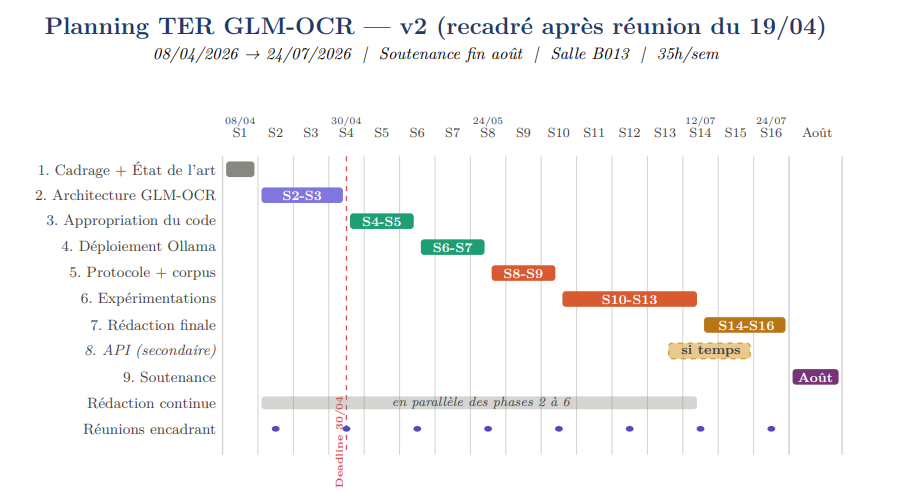
\includegraphics[width=\textwidth]{images/gantt-pre.png}
\caption{Diagramme de Gantt prévisionnel — Sujet initial GLM-OCR (avril--août 2026).}
\label{fig:gantt-prev}
\end{figure}

\subsection{Diagramme de Gantt réalisé}
\label{sec:gantt-reel}

La Figure~\ref{fig:gantt-reel} synthétise le déroulement réel du projet, intégrant la réorientation du sujet GLM-OCR vers le système RAG final.

\begin{figure}[H]
\centering
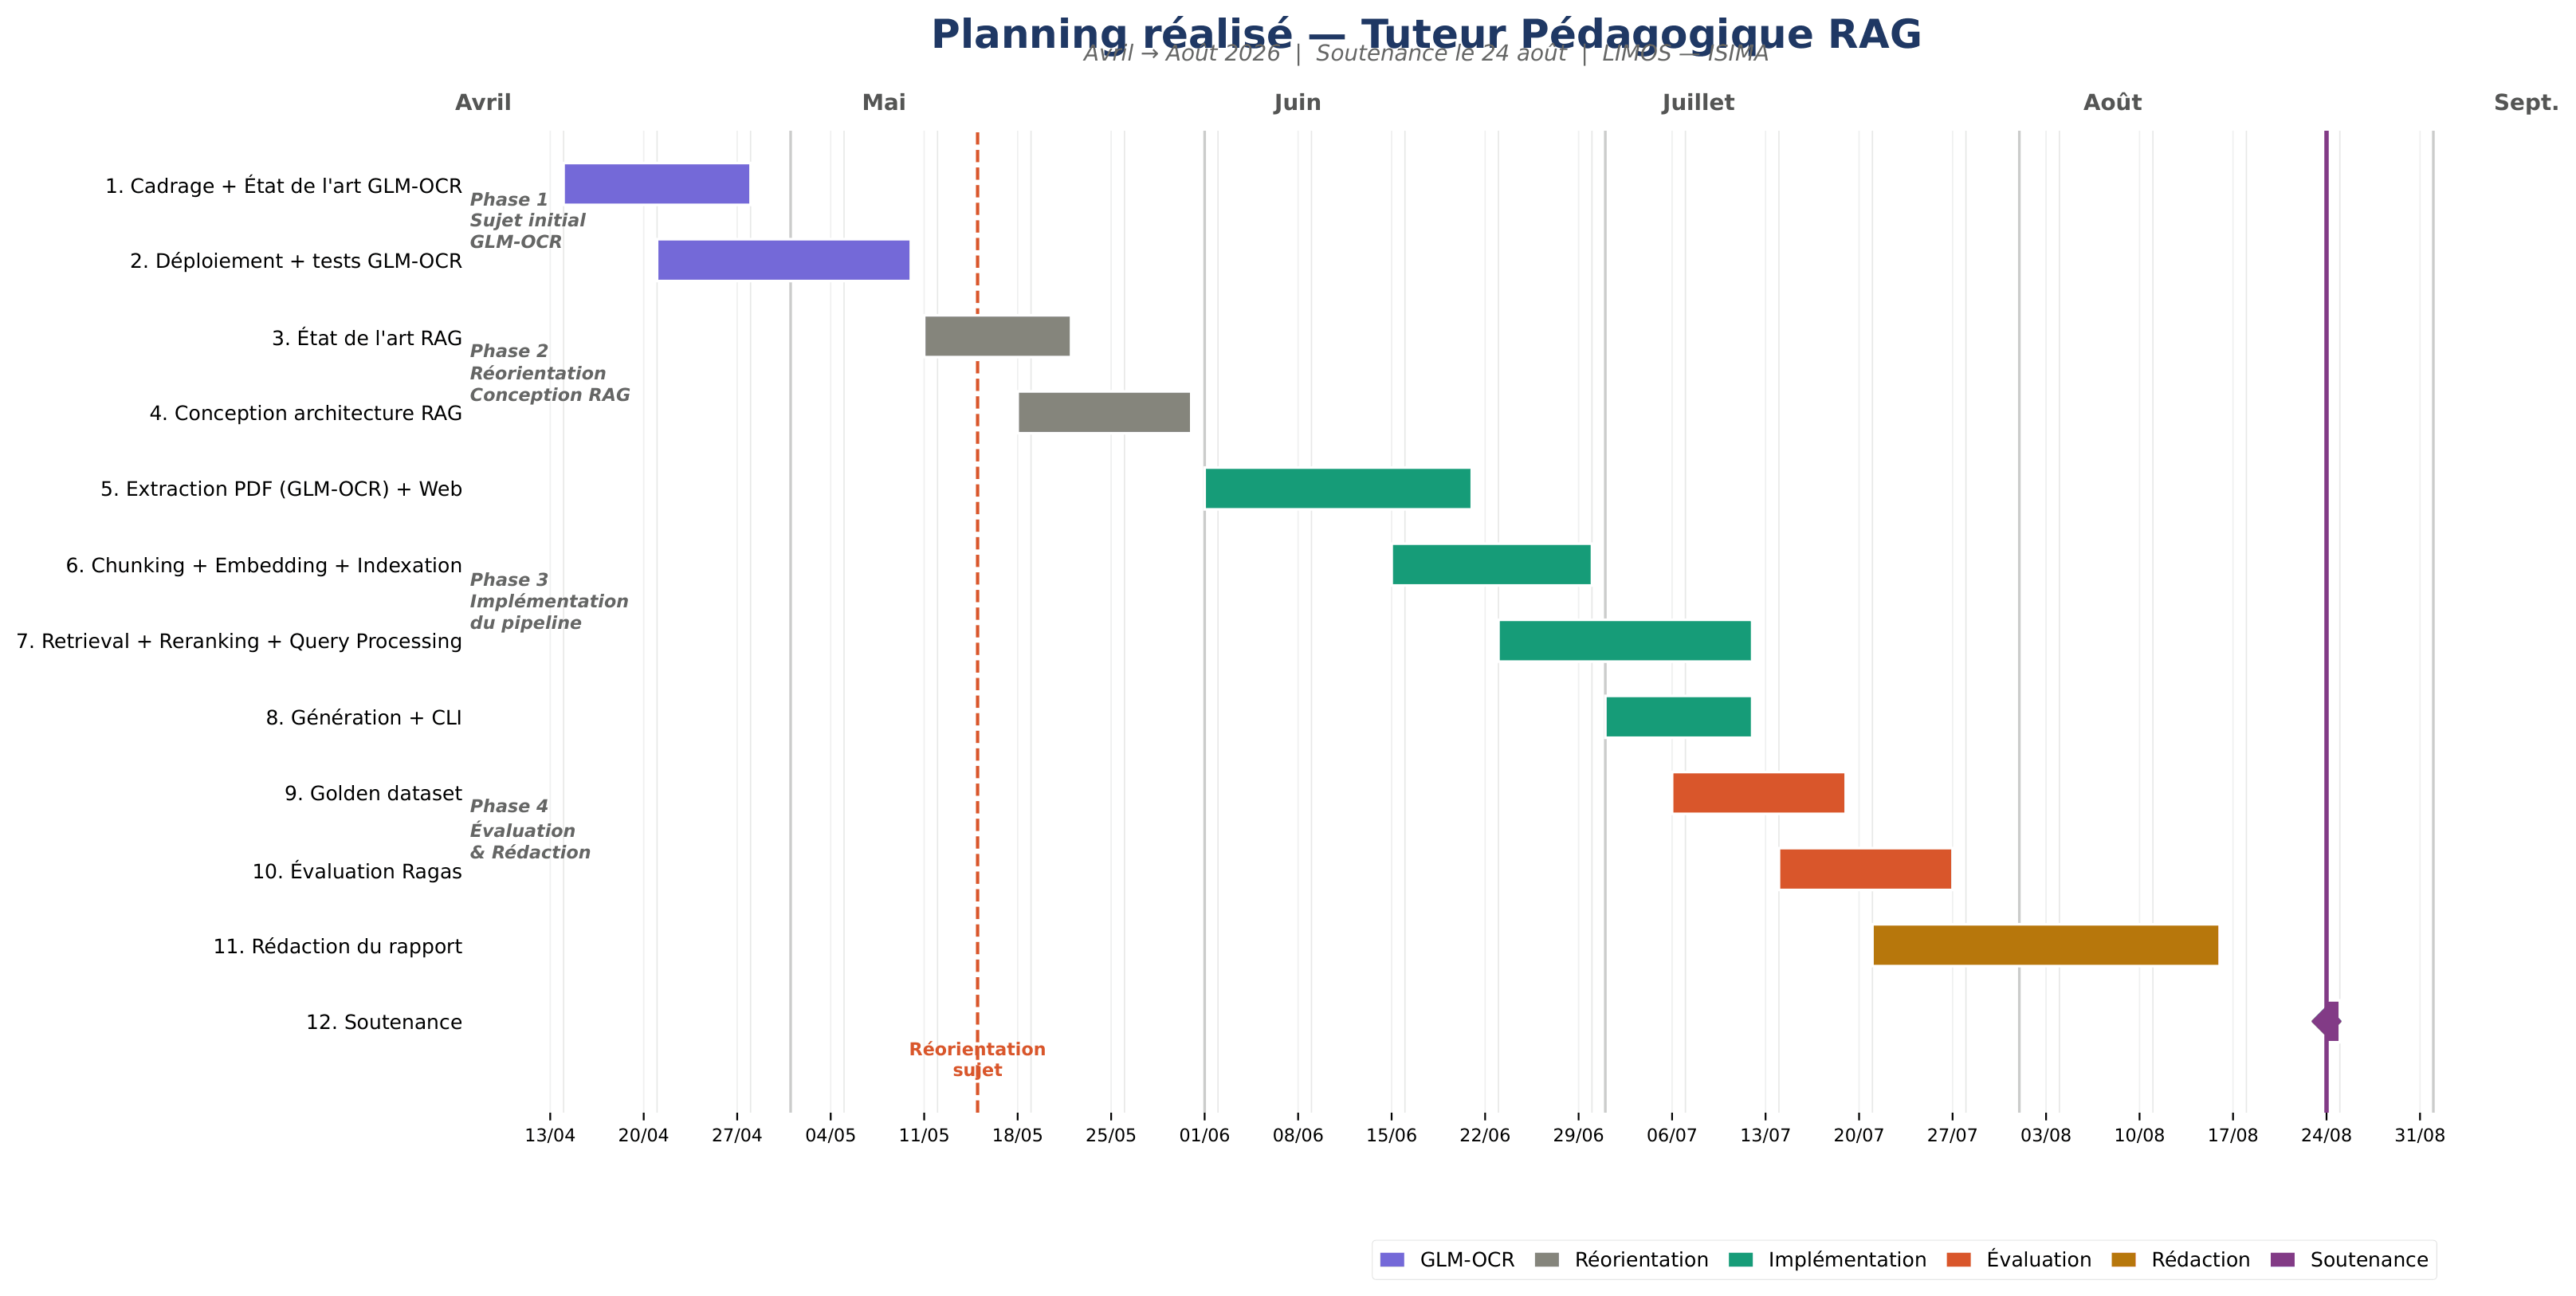
\includegraphics[width=\textwidth]{images/gantt_realise-1.png}
\caption{Diagramme de Gantt réalisé — Tuteur Pédagogique RAG (avril--août 2026). La réorientation du sujet (Phase~2) marque la transition du projet GLM-OCR initial vers le système RAG final.}
\label{fig:gantt-reel}
\end{figure}

\subsection{Analyse des écarts}
\label{sec:ecarts}

Le déroulement du projet présente un écart majeur par rapport au sujet initial~: la réorientation d'un projet centré sur GLM-OCR vers un système RAG complet. Cette section analyse cet écart ainsi que les ajustements qui en ont découlé.

\begin{table}[H]
\centering
\begin{tabularx}{\linewidth}{L{3.2cm} L{3cm} L{3cm} L{3.2cm}}
\toprule
\rowcolor{bleuPrincipal}
\textcolor{white}{\textbf{Écart}} &
\textcolor{white}{\textbf{Sujet initial}} &
\textcolor{white}{\textbf{Sujet final}} &
\textcolor{white}{\textbf{Impact}} \\
\midrule
Périmètre        & Extraction + analyse GLM-OCR & Pipeline RAG complet (extraction, retrieval, génération) & Élargissement significatif du périmètre technique \\
Corpus            & Base de données multimodale (non disponible) & Contenu web et PDF & Corpus plus accessible et maîtrisé \\
Livrable final    & Analyse critique des performances GLM-OCR & Système de tutorat pédagogique fonctionnel + évaluation quantitative & Valorisation opérationnelle du travail \\
\bottomrule
\end{tabularx}
\caption{Analyse des écarts entre le sujet initial et le projet réalisé.}
\label{tab:ecarts}
\end{table}

\paragraph{Écart principal --- Réorientation du sujet}

Le sujet initial portait exclusivement sur l'étude et l'évaluation du modèle GLM-OCR pour l'extraction de connaissances à partir de documents numérisés. L'indisponibilité de la base de données cible a conduit à une réorientation, à l'initiative du responsable de stage, vers la conception d'un système RAG complet. Cette réorientation, loin d'être un recul, a permis de~:
\begin{itemize}
  \item capitaliser sur le travail d'exploration de GLM-OCR en l'intégrant comme brique d'extraction du pipeline RAG~;
  \item élargir le périmètre technique du stage à l'ensemble de la chaîne RAG (\textit{retrieval}, \textit{reranking}, génération, évaluation)~;
  \item produire un livrable opérationnel (tuteur pédagogique fonctionnel) plutôt qu'une simple analyse comparative.
\end{itemize}

\paragraph{Impact sur le planning}

La Phase~1 (GLM-OCR) et la Phase~2 (réorientation) représentent un investissement d'environ 7 semaines sur le sujet initial et la transition. Ce temps, bien que conséquent, n'a pas été perdu puisque l'intégralité du travail sur GLM-OCR a été réutilisée dans la phase d'extraction du pipeline RAG. Le planning des Phases~3 et~4 (implémentation et évaluation du RAG) s'est déroulé conformément aux estimations, sans retard notable.

\subsection{Environnement technique}

Le projet s'appuie sur les outils et modèles suivants, tous \textit{open-weight} et exécutables localement~:

\begin{table}[H]
\centering
\begin{tabularx}{\linewidth}{L{3cm} L{4cm} L{5.5cm}}
\toprule
\rowcolor{bleuPrincipal}
\textcolor{white}{\textbf{Composant}} & \textcolor{white}{\textbf{Outil / Modèle}} & \textcolor{white}{\textbf{Rôle}} \\
\midrule
Inférence LLM   & Ollama                  & \textit{Runtime} local pour LLMs et embeddings \\
OCR             & GLM-OCR (0,9B)          & Extraction texte, tableaux, formules depuis PDF \\
Vision          & Qwen3-VL (8B)           & Interprétation des figures en langage naturel \\
Embedding       & BGE-M3 (0,6B)           & Vectorisation multilingue (dense + sparse + MV) \\
Génération      & Qwen2.5 (14B)           & Génération de réponses pédagogiques contextualisées \\
Juge            & Qwen3 (8B)              & Évaluation automatique (LLM-as-a-judge) + Juge post-génération \\
Indexation      & ChromaDB                & Base de données vectorielle \\
Retrieval       & BM25 + RRF              & Recherche hybride avec fusion de classements \\
Reranking       & BGE-Reranker-v2-m3     & Réévaluation par cross-encoder + seuil de refus pré-génération \\
Évaluation      & Ragas + DeepEval        & Métriques RAG + synthèse de golden dataset \\
Refus           & Score reranker + LLM Judge & Double mécanisme de refus (pré- et post-génération) \\
\bottomrule
\end{tabularx}
\caption{Environnement technique du projet.}
\label{tab:env-tech}
\end{table}

% =============================================================
%                 CHAPITRE 4 : ÉTAT DE L'ART
% =============================================================
\section{État de l'art~: systèmes RAG}
\label{sec:etat-art}

\subsection{Limites structurelles des modèles de langage}

Les grands modèles de langage (LLMs) ont démontré des capacités remarquables en génération de texte, en raisonnement et en résolution de problèmes complexes. Toutefois, leur utilisation directe dans un système de tutorat pédagogique se heurte à deux limites structurelles bien identifiées dans la littérature~\cite{gao2024ragsurvey,lewis2020rag}.

La première est l'\textbf{hallucination}~: un modèle peut produire une réponse plausible en apparence mais factuellement incorrecte, sans qu'aucun signal ne permette à l'utilisateur de distinguer une affirmation fondée d'une invention. Shuster~\textit{et~al.}~\cite{shuster2021hallucination} ont montré que l'intégration d'un mécanisme de récupération réduit significativement ce phénomène dans les systèmes conversationnels.

La seconde est la \textbf{fixité temporelle des connaissances}~: un modèle n'a accès qu'à ce qui figurait dans son corpus d'entraînement à une date donnée, sans possibilité de refléter un contenu de cours spécifique, mis à jour ou absent de ce corpus.

Ces deux limites sont particulièrement problématiques dans un contexte pédagogique, où une réponse erronée présentée avec assurance peut induire l'apprenant en erreur sans qu'il ait les moyens de le détecter.

\subsection{La génération augmentée par récupération (RAG)}

La \textbf{génération augmentée par récupération} (\textit{Retrieval-Augmented Generation}, RAG), introduite par Lewis~\textit{et~al.}~\cite{lewis2020rag} dans le cadre de NeurIPS~2020, répond directement à ces deux limites en ancrant la génération dans un corpus de documents contrôlé et vérifiable. Le principe fondamental consiste à découpler la \textit{connaissance} de la \textit{capacité de raisonnement}~: un corpus de documents externes fait office de mémoire consultable, tandis que le modèle de langage se limite à raisonner et à formuler une réponse à partir de ce qui lui est fourni~\cite{lewis2020rag}.

Cette séparation présente un avantage pratique majeur pour un contexte évolutif comme un cours~: mettre à jour les connaissances du système revient à mettre à jour le corpus indexé, sans réentraîner ni ajuster le modèle lui-même.

% =============================================================
\subsection{Évolution des architectures RAG}
\label{sec:evolution-rag}

Le domaine a connu une progression rapide depuis l'article fondateur de Lewis~\textit{et~al.}~\cite{lewis2020rag}, que Gao~\textit{et~al.}~\cite{gao2024ragsurvey} structurent en trois générations~: le RAG naïf, le RAG avancé et le RAG modulaire.

\subsubsection{RAG naïf (2020--2022)}

La forme la plus simple de RAG se limite à trois étapes séquentielles~: indexation du corpus en vecteurs, recherche par similarité vectorielle à partir de la requête de l'utilisateur, puis génération directe à partir des passages récupérés. Cette approche, si elle démontre le principe, se heurte rapidement à des limites pratiques~\cite{gao2024ragsurvey}~:
\begin{itemize}
  \item une recherche fondée sur un seul mécanisme (dense) peine à couvrir à la fois les correspondances exactes de vocabulaire et les reformulations sémantiques~;
  \item l'ordre de pertinence issu de la seule recherche initiale reste approximatif~;
  \item l'ensemble du contexte récupéré n'est pas nécessairement utile à la génération, un contexte surchargé pouvant au contraire diluer l'information pertinente.
\end{itemize}

\subsubsection{RAG avancé (2023--2024)}

Le RAG avancé introduit des mécanismes correctifs à chacun des points faibles du RAG naïf~\cite{gao2024ragsurvey,wang2024bestpractices}~:
\begin{itemize}
  \item \textbf{En amont de la recherche}~: reformulation de la requête (\textit{query rewriting}~\cite{ma2023queryrewriting}), décomposition de questions complexes, génération de documents hypothétiques (HyDE~\cite{gao2022hyde})~;
  \item \textbf{Au niveau de la recherche}~: recherche hybride combinant recherche lexicale et recherche dense, fusion de classements par RRF~\cite{cormack2009rrf}~;
  \item \textbf{En aval de la recherche}~: réévaluation des résultats par un modèle de \textit{reranking}~\cite{nogueira2019bert}.
\end{itemize}

C'est cette famille d'approches qui structure la conception du présent projet, avec en amont un traitement de la requête (reformulation et décomposition en sous-questions), mis en \oe{}uvre via le module de \textit{query processing}.

\subsubsection{RAG modulaire et agentique (2025--2026)}

La génération la plus récente pousse la modularité plus loin, traitant le pipeline comme un assemblage de composants interchangeables~: chaque phase (extraction, \textit{chunking}, \textit{embedding}, recherche, \textit{reranking}, génération) est conçue comme un module indépendant, remplaçable sans impact sur les autres~\cite{gao2024ragsurvey}. Cette philosophie est celle qui guide l'architecture du présent projet.

En parallèle, le paradigme \textbf{RAG agentique} émerge~\cite{singh2025agenticrag}~: des agents fondés sur des LLMs orchestrent dynamiquement le pipeline, décidant à chaque étape s'il faut reformuler la requête, relancer la recherche, ou corriger la réponse générée. Les architectures CRAG (\textit{Corrective RAG}) et Self-RAG illustrent cette tendance, le modèle évaluant lui-même la pertinence des passages récupérés et la fidélité de sa propre réponse avant de la retourner à l'utilisateur. Le TREC~2025 RAG Track~\cite{trec2025rag} a formalisé cette évaluation à grande échelle, avec plus de 150~soumissions évaluées sur la pertinence, la complétude, et l'attribution des réponses.

% =============================================================
\subsection{État de l'art par phase du pipeline}
\label{sec:etat-art-phases}

Cette section passe en revue l'état de l'art pour chaque phase du pipeline RAG, en se concentrant sur les composantes pertinentes pour le projet.

% ------- CHUNKING -------
\subsubsection{Stratégies de découpage (\textit{chunking})}

Le découpage d'un corpus en unités indexables conditionne directement la qualité du \textit{retrieval} en aval. Lu~\textit{et~al.}~\cite{lu2025hichunk} montrent que la méthode de \textit{chunking} impacte significativement chaque composante du pipeline RAG, de la qualité de la recherche à la fidélité de la génération. Reuter~\textit{et~al.}~\cite{reuter2026chunking} confirment que les stratégies structurellement informées surpassent de manière consistante les découpages à taille fixe, tout en soulignant le surcoût computationnel qu'elles impliquent.

La littérature distingue cinq familles principales de stratégies.

\paragraph{Découpage à taille fixe}

L'approche la plus simple consiste à segmenter le texte en blocs de taille constante (en \textit{tokens} ou en caractères), avec un chevauchement optionnel entre blocs consécutifs. Simple à mettre en \oe{}uvre, elle présente un défaut majeur~: la frontière de découpe ignore la structure sémantique du texte, risquant de fragmenter une unité de sens~\cite{smith2024chunking}.

\paragraph{Découpage récursif}

Le découpage récursif (\textit{recursive text splitting}) utilise une hiérarchie de séparateurs (paragraphes, puis phrases, puis caractères) appliquée récursivement jusqu'à obtenir des blocs de taille cible. Il respecte mieux la structure syntaxique du texte, mais reste aveugle à la structure sémantique du document (sections, sous-sections)~\cite{langchain2023}.

\paragraph{Découpage \textit{structure-aware}}

Le découpage \textit{structure-aware} s'appuie directement sur la hiérarchie de titres et sections du document pour déterminer les frontières de découpe. Chaque section ou sous-section constitue un \textit{chunk} naturel. Cette approche préserve l'unité sémantique mais peut produire des \textit{chunks} de tailles très hétérogènes~\cite{yepes2024chunking}.

\paragraph{Découpage hiérarchique parent-enfant}

Le découpage parent-enfant propose une réponse au compromis granularité/contexte~: plutôt que de chercher une taille de \textit{chunk} unique, il sépare ces deux granularités en deux niveaux de \textit{chunks} distincts, reliés entre eux~\cite{langchain2023}. Les \textit{chunks} enfants, courts et précis, servent de granularité pour la recherche~; le \textit{chunk} parent associé, plus large, fournit le contexte complet transmis à la génération. Cette approche a été validée dans le cadre de SemEval~2026 Task~8 par le système H-RAG~\cite{hrag2026semeval}, qui confirme l'importance de l'agrégation au niveau parent pour la qualité de la génération dans les systèmes RAG multi-tours.

\paragraph{Découpage sémantique}

Le découpage sémantique utilise les \textit{embeddings} eux-mêmes pour déterminer les frontières de découpe~: un changement brusque de similarité entre phrases consécutives signale une rupture thématique. Qu~\textit{et~al.}~\cite{qu2025semantic} ont toutefois montré que le gain de performance par rapport aux méthodes plus simples ne justifie pas toujours le surcoût computationnel, en particulier pour des corpus structurés.

\begin{table}[H]
\centering
\small
\begin{tabularx}{\linewidth}{L{2.8cm} C{2cm} C{2.2cm} C{2.2cm} L{3cm}}
\toprule
\rowcolor{bleuPrincipal}
\textcolor{white}{\textbf{Stratégie}} &
\textcolor{white}{\textbf{Granularité}} &
\textcolor{white}{\textbf{Contexte}} &
\textcolor{white}{\textbf{Complexité}} &
\textcolor{white}{\textbf{Limite principale}} \\
\midrule
Taille fixe          & Fine     & Faible    & Triviale    & Fragmentation sémantique \\
Récursif             & Fine     & Moyen     & Faible      & Aveugle à la structure \\
\textit{Structure-aware} & Variable & Fort  & Moyenne     & Tailles hétérogènes \\
\rowcolor{bleuAccent}
\textbf{Parent-enfant} & \textbf{Fine + large} & \textbf{Fort} & \textbf{Moyenne} & \textbf{Complexité d'indexation} \\
Sémantique           & Variable & Fort      & Élevée      & Coût computationnel \\
\bottomrule
\end{tabularx}
\caption{Synthèse comparative des stratégies de \textit{chunking}. La stratégie retenue (parent-enfant) est mise en évidence.}
\label{tab:chunking}
\end{table}

% ------- EMBEDDING -------
\subsubsection{Modèles d'\textit{embedding}}

Le choix d'un modèle d'\textit{embedding} détermine la qualité de la recherche sémantique. Le paysage des modèles multilingues \textit{open-weight} a connu une évolution rapide, portée par les \textit{benchmarks} de référence MTEB~\cite{muennighoff2023mteb} et sa version étendue MMTEB~\cite{enevoldsen2025mmteb}, couvrant plus de 500~tâches d'évaluation sur plus de 250~langues.

\paragraph{Évolution des modèles}

Les premiers modèles d'\textit{embedding} multilingues (mBERT, XLM-R) produisaient des représentations de qualité limitée pour la recherche. L'introduction de modèles entraînés spécifiquement pour le \textit{retrieval}, comme E5~\cite{wang2024e5} et GTE~\cite{li2023gte}, a marqué un premier saut de performance. La famille BGE (\textit{BAAI General Embedding}) a ensuite poussé les performances sur les \textit{benchmarks} multilingues, culminant avec \textbf{BGE-M3}~\cite{chen2024bgem3}, qui unifie trois modes de \textit{retrieval} (dense, sparse et multi-vecteurs) dans un seul modèle, supportant plus de 100~langues avec des entrées jusqu'à 8\,192~\textit{tokens}.

Plus récemment, la famille \textbf{Qwen3-Embedding}~\cite{zhang2025qwen3embedding} (Alibaba), publiée en juin~2025, occupe la première place du classement MMTEB multilingue avec un score de 70,58 pour la variante 8B (au 5~juin~2025). La série est disponible en trois tailles (0.6B, 4B, 8B) et inclut également des modèles de \textit{reranking}, héritant des capacités multilingues et de raisonnement de la série Qwen3.

\paragraph{Tableau comparatif}

\begin{table}[H]
\centering
\small
\begin{tabularx}{\linewidth}{L{3cm} C{1.3cm} C{1.3cm} C{2.2cm} C{1.5cm} C{1.5cm}}
\toprule
\rowcolor{bleuPrincipal}
\textcolor{white}{\textbf{Modèle}} &
\textcolor{white}{\textbf{Dim.}} &
\textcolor{white}{\textbf{Langues}} &
\textcolor{white}{\textbf{Modes}} &
\textcolor{white}{\textbf{Contexte}} &
\textcolor{white}{\textbf{Local}} \\
\midrule
E5-multilingual       & 1024 & 100+  & Dense      & 514   & Oui \\
GTE-Qwen2-7B          & 1536 & 30+   & Dense      & 32768 & Oui \\
\rowcolor{bleuAccent}
\textbf{BGE-M3}       & \textbf{1024} & \textbf{100+} & \textbf{Dense+sparse+MV} & \textbf{8192} & \textbf{Oui} \\
Qwen3-Embedding-8B    & 1024 & 100+  & Dense      & 32768 & Oui \\
text-embedding-3      & 3072 & 100+  & Dense      & 8191  & Non (API) \\
Gemini-Embedding      & 3072 & 100+  & Dense      & 8192  & Non (API) \\
\bottomrule
\end{tabularx}
\caption{Synthèse comparative des modèles d'\textit{embedding} multilingues (mi-2026). Le modèle retenu (BGE-M3) est mis en évidence. MV = multi-vecteurs.}
\label{tab:embedding}
\end{table}

% ------- RETRIEVAL -------
\subsubsection{Mécanismes de recherche (\textit{retrieval})}

La phase de \textit{retrieval} vise à retrouver, pour chaque requête, les passages les plus pertinents du corpus indexé. Trois familles de mécanismes coexistent, avec une tendance marquée vers leur combinaison~\cite{gao2024ragsurvey,wang2024bestpractices}.

\paragraph{Recherche lexicale (sparse)}

La recherche lexicale repose sur la correspondance exacte de termes entre la requête et les documents. \textbf{BM25}, issu du \textit{Probabilistic Relevance Framework}~\cite{robertson2009bm25}, reste à ce jour l'algorithme de référence en recherche lexicale. Strich~\textit{et~al.}~\cite{strich2026bm25} ont montré en~2026 que, sur des documents financiers à terminologie précise, BM25 surpasse la recherche dense avec text-embedding-3-large sur la quasi-totalité des métriques --- un résultat qui remet en cause l'hypothèse courante de la domination universelle de la recherche dense.

\paragraph{Recherche dense (sémantique)}

La recherche dense encode la requête et les documents dans un même espace vectoriel, puis classe les documents par similarité cosinus avec le vecteur de la requête. Cette approche, rendue praticable par les modèles d'\textit{embedding} pré-entraînés (cf.~section précédente), capte les reformulations et les relations sémantiques, mais peut manquer une correspondance lexicale exacte sur un terme technique~\cite{chen2024bgem3}.

\paragraph{Recherche hybride et fusion}

La recherche hybride combine les deux mécanismes pour exploiter leurs forces complémentaires. La principale difficulté technique réside dans la fusion des classements~: les scores BM25 et les scores de similarité cosinus ne sont pas directement comparables, car ils opèrent sur des échelles différentes.

La \textbf{fusion de rang réciproque} (\textit{Reciprocal Rank Fusion}, RRF), introduite par Cormack~\textit{et~al.}~\cite{cormack2009rrf} à SIGIR~2009, contourne ce problème en s'appuyant uniquement sur la \textit{position} de chaque résultat dans chaque classement, indépendamment des scores bruts. Le score RRF d'un document~$d$ est défini par~:
\begin{equation}
  \text{RRF}(d) = \sum_{r \in \mathcal{R}} \frac{1}{k + \operatorname{rang}_r(d)}
  \label{eq:rrf}
\end{equation}
où~$\mathcal{R}$ est l'ensemble des mécanismes de recherche, $\operatorname{rang}_r(d)$ la position du document~$d$ dans le classement du mécanisme~$r$, et~$k$ une constante de lissage (typiquement~60). Cormack~\textit{et~al.} ont montré que cette méthode surpasse les approches de fusion par apprentissage et les méthodes de type Condorcet sur les \textit{benchmarks} TREC. Strich~\textit{et~al.}~\cite{strich2026bm25} confirment en~2026 qu'un pipeline hybride en deux étapes (recherche hybride + \textit{reranking} neuronal) atteint les meilleures performances (Recall@5~=~0,816, MRR@3~=~0,605), surpassant toutes les méthodes à une seule étape.

\paragraph{Réévaluation par \textit{cross-encoder} (\textit{reranking})}

La recherche initiale (lexicale, dense ou hybride) est optimisée pour parcourir rapidement l'ensemble du corpus, mais ne garantit pas un classement fin des résultats. Une étape de réévaluation par \textbf{\textit{cross-encoder}} affine ce classement en comparant \textit{conjointement} la requête et chaque passage candidat, plutôt que des représentations vectorielles précalculées indépendamment.

Nogueira et Cho~\cite{nogueira2019bert} ont démontré en~2019 que des modèles BERT \textit{fine-tunés} comme \textit{cross-encoders} surpassaient largement les méthodes classiques de \textit{reranking} sur le \textit{benchmark} MS~MARCO. Le principe a depuis été étendu à des modèles spécialisés multilingues~: \textbf{BGE-reranker-v2-m3}~\cite{xiao2024bge} constitue une référence en contexte multilingue. Plus récemment, la série \textbf{Qwen3-Reranker}~\cite{zhang2025qwen3embedding}, publiée conjointement avec Qwen3-Embedding, propose des modèles de \textit{reranking} en 0.6B et 8B qui excellent dans les scénarios de recherche textuelle multilingue.

Fensore~\textit{et~al.}~\cite{fensore2025liverag} illustrent le compromis coût/qualité du \textit{reranking} dans le cadre du LiveRAG Challenge~2025~: le \textit{reranking} par RankLLaMA améliore le MAP de 0,523 à 0,797 (amélioration relative de~52\,\%), mais au prix d'un temps d'inférence passant de 1,74\,s à 84\,s par question.

\begin{table}[H]
\centering
\small
\begin{tabularx}{\linewidth}{L{3cm} L{3.5cm} L{3.5cm} C{2.5cm}}
\toprule
\rowcolor{bleuPrincipal}
\textcolor{white}{\textbf{Mécanisme}} &
\textcolor{white}{\textbf{Forces}} &
\textcolor{white}{\textbf{Limites}} &
\textcolor{white}{\textbf{Complexité}} \\
\midrule
BM25 (lexical)        & Correspondances exactes, termes techniques   & Aveugle au sens        & $\mathcal{O}(n)$ \\
Dense (BGE-M3)        & Reformulations, synonymes                     & Peut manquer l'exact   & $\mathcal{O}(n)$ \\
\rowcolor{bleuAccent}
\textbf{Hybride + RRF} & \textbf{Complémentarité lexical/sémant.}      & \textbf{Double index}  & $\mathcal{O}(n)$ \\
\textit{Cross-encoder}& Classement très précis                        & Coût quadratique       & $\mathcal{O}(k \cdot \ell^2)$ \\
\bottomrule
\end{tabularx}
\caption{Synthèse comparative des mécanismes de \textit{retrieval}. L'approche retenue combine les trois lignes~: hybride + RRF + \textit{cross-encoder}.}
\label{tab:retrieval}
\end{table}

% ------- GÉNÉRATION -------
\subsubsection{Génération contrainte par le contexte}

La génération dans un système RAG doit être explicitement contrainte pour exploiter le contexte récupéré plutôt que les connaissances internes du modèle. Cette contrainte se matérialise par un \textit{prompt de génération} qui impose un ancrage strict (\textit{grounding})~: la réponse doit s'appuyer exclusivement sur le contexte fourni, avec un refus explicite en l'absence d'information pertinente~\cite{gao2024ragsurvey}.

\paragraph{Évolution des LLMs déployables localement}

Le paysage des modèles de langage exploitables localement a connu une évolution rapide. La famille \textbf{Qwen} (Alibaba), déployée via des \textit{runtimes} d'inférence locale comme Ollama ou vLLM, illustre cette progression~: Qwen2.5~\cite{qwen2024qwen25} a constitué un choix de référence en~2024--2025 pour le RAG local, tandis que Qwen3~\cite{qwen2025qwen3}, publié en mai~2025, apporte une fenêtre de contexte élargie, un support multilingue renforcé, et un mode de raisonnement hybride (\textit{thinking}/\textit{non-thinking}), sans coût supplémentaire pour un déploiement local.

\paragraph{Techniques d'amélioration de la génération}

La \textbf{reformulation de requête} (\textit{query rewriting}) consiste à réécrire ou décomposer la requête de l'utilisateur avant de l'envoyer au \textit{retrieval}, afin de corriger une formulation ambiguë ou sous-spécifiée. Ma~\textit{et~al.}~\cite{ma2023queryrewriting} ont montré que cette technique améliore significativement les performances en question-réponse ouverte. Dans ce projet, elle est mise en \oe{}uvre par le module de \textit{query processing}, qui reformule la question et la décompose en sous-questions indépendantes lorsque nécessaire. 

% ------- ÉVALUATION -------
\subsubsection{Évaluation des systèmes RAG}

L'évaluation d'un système RAG se distingue de l'évaluation d'un modèle de langage seul par la nécessité d'évaluer conjointement deux composantes~: la qualité du \textit{retrieval} et la qualité de la génération~\cite{es2024ragas}.

\paragraph{Métriques de \textit{retrieval}}

Les métriques de rang évaluent la capacité du système à retrouver les passages pertinents~:
\begin{itemize}
  \item \textbf{Hit@k}~: proportion des requêtes pour lesquelles au moins un passage pertinent figure parmi les~$k$ premiers résultats~;
  \item \textbf{MRR} (\textit{Mean Reciprocal Rank})~: moyenne de l'inverse du rang du premier passage pertinent~;
  \item \textbf{Précision et rappel du contexte}~: proportion des passages récupérés qui sont pertinents, et proportion des passages pertinents qui sont récupérés.
\end{itemize}

\paragraph{Métriques de génération}

Les métriques de génération, fondées sur le principe du \textit{modèle-juge} (\textit{LLM-as-a-judge}), évaluent la qualité de la réponse produite~:
\begin{itemize}
  \item \textbf{Fidélité} (\textit{faithfulness})~: la réponse est-elle fidèle au contexte fourni, sans ajout d'information non présente dans les passages récupérés~?
  \item \textbf{Pertinence de la réponse} (\textit{answer relevancy})~: la réponse adresse-t-elle bien la question posée~?
  \item \textbf{Exactitude factuelle} (\textit{factual correctness})~: la réponse est-elle factuellement correcte par rapport à la vérité terrain~?
\end{itemize}

\paragraph{\textit{Frameworks} d'évaluation}

Deux \textit{frameworks} structurent aujourd'hui cette évaluation~:

\textbf{Ragas} (\textit{Retrieval Augmented Generation Assessment}), introduit par Es~\textit{et~al.}~\cite{es2024ragas} et présenté à EACL~2024, est conçu spécifiquement pour les systèmes RAG. Il fournit une suite de métriques (fidélité, pertinence de la réponse, précision et rappel du contexte) calculées sans annotation humaine, via un modèle de langage juge. Sa légèreté et sa spécialisation RAG en font un choix naturel pour une évaluation rapide.

\textbf{DeepEval}~\cite{deepeval2024} est un \textit{framework} plus généraliste de test de systèmes fondés sur des LLMs, incluant des métriques RAG comparables à celles de Ragas, ainsi qu'un \textbf{synthétiseur de données de test} permettant de générer automatiquement un jeu de questions-réponses de référence (\textit{golden dataset}) à partir du corpus lui-même. Ce dernier outil permet de constituer un jeu d'évaluation sans annotation manuelle exhaustive.

\begin{table}[H]
\centering
\small
\begin{tabularx}{\linewidth}{L{2.5cm} L{3.5cm} L{3.5cm} C{3cm}}
\toprule
\rowcolor{bleuPrincipal}
\textcolor{white}{\textbf{\textit{Framework}}} &
\textcolor{white}{\textbf{Forces}} &
\textcolor{white}{\textbf{Limites}} &
\textcolor{white}{\textbf{Synthèse de données}} \\
\midrule
\rowcolor{bleuAccent}
\textbf{Ragas} $\star$  & Spécialisé RAG, léger, \textit{reference-free}   & Pas de synthétiseur natif        & Non \\
DeepEval $\star\star$ & Métriques RAG + généralistes, synthétiseur de \textit{golden dataset} & Plus lent pour le calcul des métriques & \textbf{Oui} \\
\bottomrule
\end{tabularx}
\caption{Synthèse comparative des \textit{frameworks} d'évaluation RAG. $\star$~= retenu pour le calcul des métriques. $\star\star$~= retenu pour la synthèse du \textit{golden dataset}.}
\label{tab:eval}
\end{table}

% =============================================================
\subsection{Tensions du domaine et positionnement du projet}
\label{sec:tensions}

La revue précédente fait émerger plusieurs \textbf{tensions} que les approches existantes n'adressent pas toujours simultanément~:

\begin{itemize}
  \item \textbf{Performance vs. déployabilité locale.} Les systèmes RAG les plus performants reposent sur des modèles propriétaires (GPT-4o pour la génération, text-embedding-3 pour l'\textit{embedding}, Cohere pour le \textit{reranking}), incompatibles avec une contrainte de déploiement local à coût nul.

  \item \textbf{Précision lexicale vs. compréhension sémantique.} Les mécanismes de recherche lexicale et dense présentent des forces complémentaires mais des faiblesses symétriques~\cite{strich2026bm25}. Leur combinaison (recherche hybride) est bien documentée mais introduit la difficulté supplémentaire de la fusion de classements hétérogènes.

  \item \textbf{Granularité de recherche vs. richesse de contexte.} Un \textit{chunk} court améliore la précision de la recherche mais appauvrit le contexte fourni à la génération~\cite{lu2025hichunk}. Le découpage parent-enfant adresse ce compromis mais augmente la complexité de l'indexation.

  \item \textbf{Qualité de réévaluation vs. coût d'inférence.} Le \textit{reranking} par \textit{cross-encoder} améliore significativement le classement~\cite{nogueira2019bert} mais son coût peut être prohibitif~: Fensore~\textit{et~al.}~\cite{fensore2025liverag} mesurent un facteur~48$\times$ sur le temps d'inférence.

  \item \textbf{Rigueur d'évaluation vs. coût de constitution des données de test.} L'évaluation rigoureuse d'un système RAG nécessite un jeu de données de référence, dont la constitution manuelle est coûteuse. Les synthétiseurs automatiques (DeepEval) offrent une alternative, au prix d'un temps de calcul plus important~\cite{deepeval2024}.
\end{itemize}

\subsection*{Positionnement du projet}

Les choix opérés dans ce projet s'inscrivent dans ce panorama avec une contrainte transversale~: un déploiement entièrement local, sans coût d'API, la performance étant jugée à l'aune de ce qui est disponible à la date de rédaction (mi-2026).

Pour l'extraction, \textsc{GLM-OCR}~\cite{glmocr2026} a été retenu pour sa capacité native à traiter texte, tableaux et formules dans un pipeline unique, exécutable localement. L'interprétation des figures s'appuie sur \textbf{Qwen3-VL-8B}~\cite{qwen2025qwen3vl}, choisie comme meilleur compromis entre capacité de raisonnement visuel et coût d'inférence local.

Pour l'ingestion, le \textbf{découpage parent-enfant} a été retenu afin de concilier précision de recherche et richesse contextuelle, conformément aux résultats de Lu~\textit{et~al.}~\cite{lu2025hichunk} et du système H-RAG~\cite{hrag2026semeval}~; \textbf{BGE-M3}~\cite{chen2024bgem3} reste le modèle d'\textit{embedding} utilisé, son rapport qualité-coût demeurant pertinent pour ce POC bien que des alternatives plus récentes (Qwen3-Embedding~\cite{zhang2025qwen3embedding}) occupent le haut des classements ouverts~; \textbf{ChromaDB} a été retenu pour l'indexation vectorielle, suffisant à l'échelle du corpus traité.

Pour le \textit{retrieval}, la combinaison \textbf{BM25}~\cite{robertson2009bm25} et \textbf{recherche dense} (BGE-M3), fusionnée par \textbf{RRF}~\cite{cormack2009rrf} puis réévaluée par un \textbf{\textit{cross-encoder}}~\cite{nogueira2019bert,xiao2024bge}, correspond à l'architecture hybride en deux étapes validée par Strich~\textit{et~al.}~\cite{strich2026bm25} comme la plus performante. Le traitement de la requête (\textit{query processing}) complète la chaîne en amont.

Pour la génération, \textbf{Qwen2.5}~\cite{qwen2024qwen25} via Ollama a été conservé comme choix fonctionnel et gratuit, Qwen3~\cite{qwen2025qwen3} étant identifié comme évolution possible sans remise en cause de l'architecture.

Enfin, pour l'évaluation, le \textbf{synthétiseur de DeepEval}~\cite{deepeval2024} a été utilisé pour constituer le \textit{golden dataset} à partir du corpus, tandis que le calcul des métriques repose sur \textbf{Ragas}~\cite{es2024ragas}, retenu pour sa légèreté et sa spécialisation RAG.

% =============================================================
%                CHAPITRE 5 : MÉTHODOLOGIE
% =============================================================
\section{Méthodologie}
\label{sec:methodologie}

\subsection{Analyse des besoins}

\subsubsection{Contexte et nature des données}

Le projet vise à construire un système de tutorat pédagogique basé sur une architecture RAG, exploitant deux catégories de sources documentaires~: des documents PDF (supports de cours natifs ou scannés) et des pages web (ressources pédagogiques complémentaires). Ces deux types de sources présentent des caractéristiques et des contraintes d'extraction distinctes qui structurent l'ensemble des choix techniques en amont.

Les documents PDF combinent du texte structuré, des formules mathématiques, des tableaux, et des figures (schémas, graphiques, captures d'écran). Les pages web combinent du texte, des extraits de code, et une structure HTML porteuse de bruit (menus, liens, éléments décoratifs) qu'il convient d'écarter.

\subsubsection{Exigences fonctionnelles}

De cette nature des données découlent des exigences d'extraction spécifiques à chaque source~:

Pour les PDF~: (i)~extraction du texte brut, (ii)~extraction structurée des formules mathématiques et des tableaux, (iii)~interprétation sémantique des figures par transcription en langage naturel.

Pour les sites web~: (i)~extraction du texte et conversion en un format structuré exploitable, (ii)~extraction des blocs de code et des formules mathématiques, (iii)~élimination du bruit non pédagogique.

\subsubsection{Contraintes du projet}

Le projet est mené dans un cadre de preuve de concept (POC), avec les contraintes suivantes~:

\begin{itemize}
  \item \textbf{Déploiement local}~: le pipeline s'exécute entièrement sur l'infrastructure locale disponible, sans appel à des services distants. Ce choix répond à une logique de maîtrise de l'infrastructure et de contrôle des coûts --- les données utilisées étant des contenus pédagogiques déjà librement accessibles, sans caractère sensible.
  \item \textbf{Contrainte budgétaire}~: recours exclusif à des outils et modèles \textit{open-weight}, sans coût d'API, la performance étant évaluée à l'aune de ce qui est disponible et exploitable localement à la date de rédaction (mi-2026).
  \item \textbf{Contrainte matérielle}~: le pipeline doit rester exécutable sur le matériel partagé disponible (GPU NVIDIA H100 NVL, 95 Go de VRAM), ce qui oriente vers des modèles de taille raisonnable plutôt que vers les plus gros modèles disponibles.
\end{itemize}

Ces contraintes orientent dès ce stade les grandes décisions d'architecture (outils \textit{open-weight}, dimensionnement des modèles) détaillées dans les parties Conception et Implémentation.

\subsection{Conception}

\subsubsection{Principes de conception}

Les contraintes identifiées dans l'analyse des besoins orientent directement les principes qui structurent la conception du système.

Le premier principe est la \textbf{modularité}~: chaque phase du pipeline (extraction, normalisation, ingestion, \textit{retrieval}, génération) est conçue comme un composant indépendant, remplaçable sans impact sur les autres. Cette modularité permet de faire évoluer un choix d'outil ou de modèle à mesure que l'état de l'art progresse, sans remettre en cause l'architecture globale.

Le second principe est la \textbf{séparation entre extraction et traitement}~: les données brutes (PDF, pages web) sont d'abord converties vers un format normalisé commun, avant toute opération de préparation à la recherche. Cette séparation évite que les spécificités de chaque source ne se propagent dans les étapes en aval.

Le troisième principe est la \textbf{testabilité par étape}~: chaque phase du pipeline doit pouvoir être validée indépendamment (qualité d'extraction, pertinence du \textit{chunking}, précision du \textit{retrieval}, fidélité de la génération), ce qui conditionne directement la phase d'évaluation présentée plus loin.

\subsubsection{Vue d'ensemble de l'architecture}

Le pipeline se structure en deux temps~: une phase de préparation des données, exécutée une seule fois en amont, et une phase d'exécution, déclenchée à chaque requête de l'utilisateur. La phase de préparation (Extraction $\to$ Normalisation $\to$ Ingestion) convertit les sources brutes en une base vectorielle indexée. La phase d'exécution (Requête $\to$ \textit{Retrieval} $\to$ Génération $\to$ Réponse) part d'une question de l'utilisateur, retrouve les passages pertinents, puis génère une réponse contextualisée.

\begin{figure}[H]
\centering
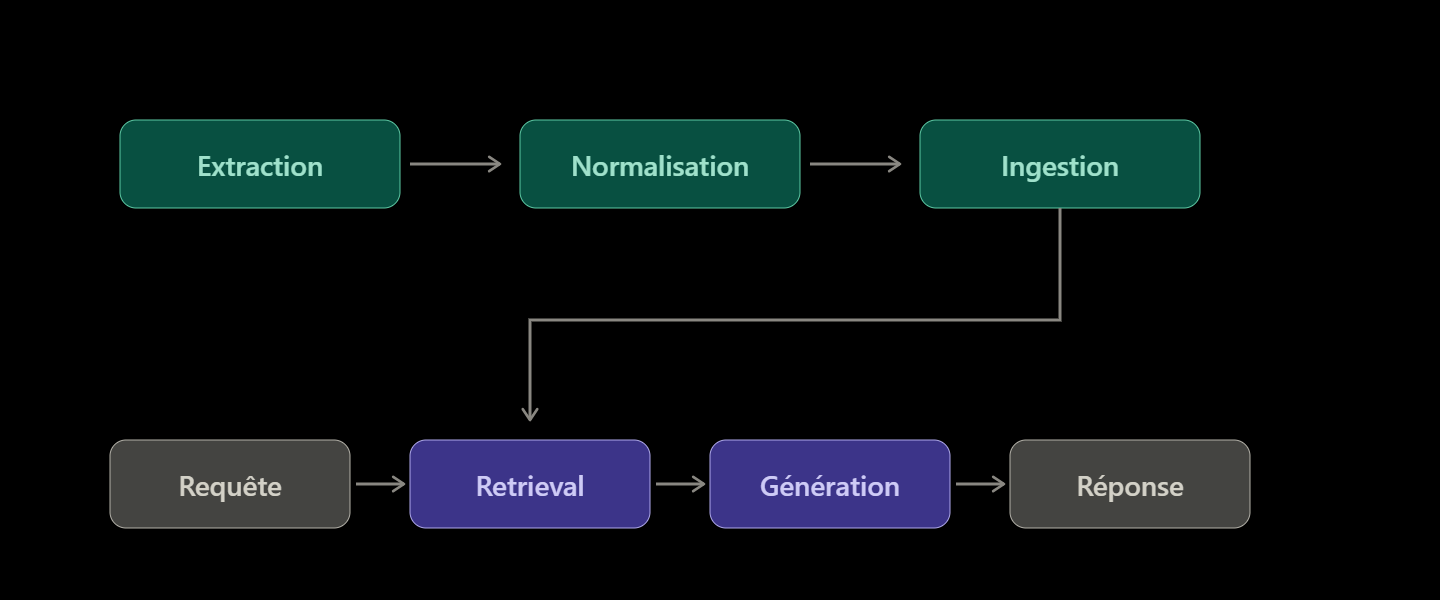
\includegraphics[width=\linewidth]{images/pipeline_global.png}
\caption{Vue d'ensemble de l'architecture. Vert~= phase de préparation (\textit{offline}), gris~= interface utilisateur, violet~= traitement de la requête.}
\label{fig:pipeline-global}
\end{figure}

\subsubsection{Conception du traitement des données}

Le traitement des données se compose de deux pipelines d'extraction distincts --- l'un pour les PDF, l'autre pour les pages web --- qui convergent vers une étape commune de normalisation, garantissant que la suite du système manipule un format homogène, indépendamment de la source d'origine. Le pipeline PDF traite trois natures de contenu en parallèle~: le texte brut, les éléments structurés (formules mathématiques, tableaux), et les figures. Le pipeline web traite le texte, les blocs de code, les formules mathématiques, et élimine le bruit structurel du HTML.

\begin{figure}[H]
\centering
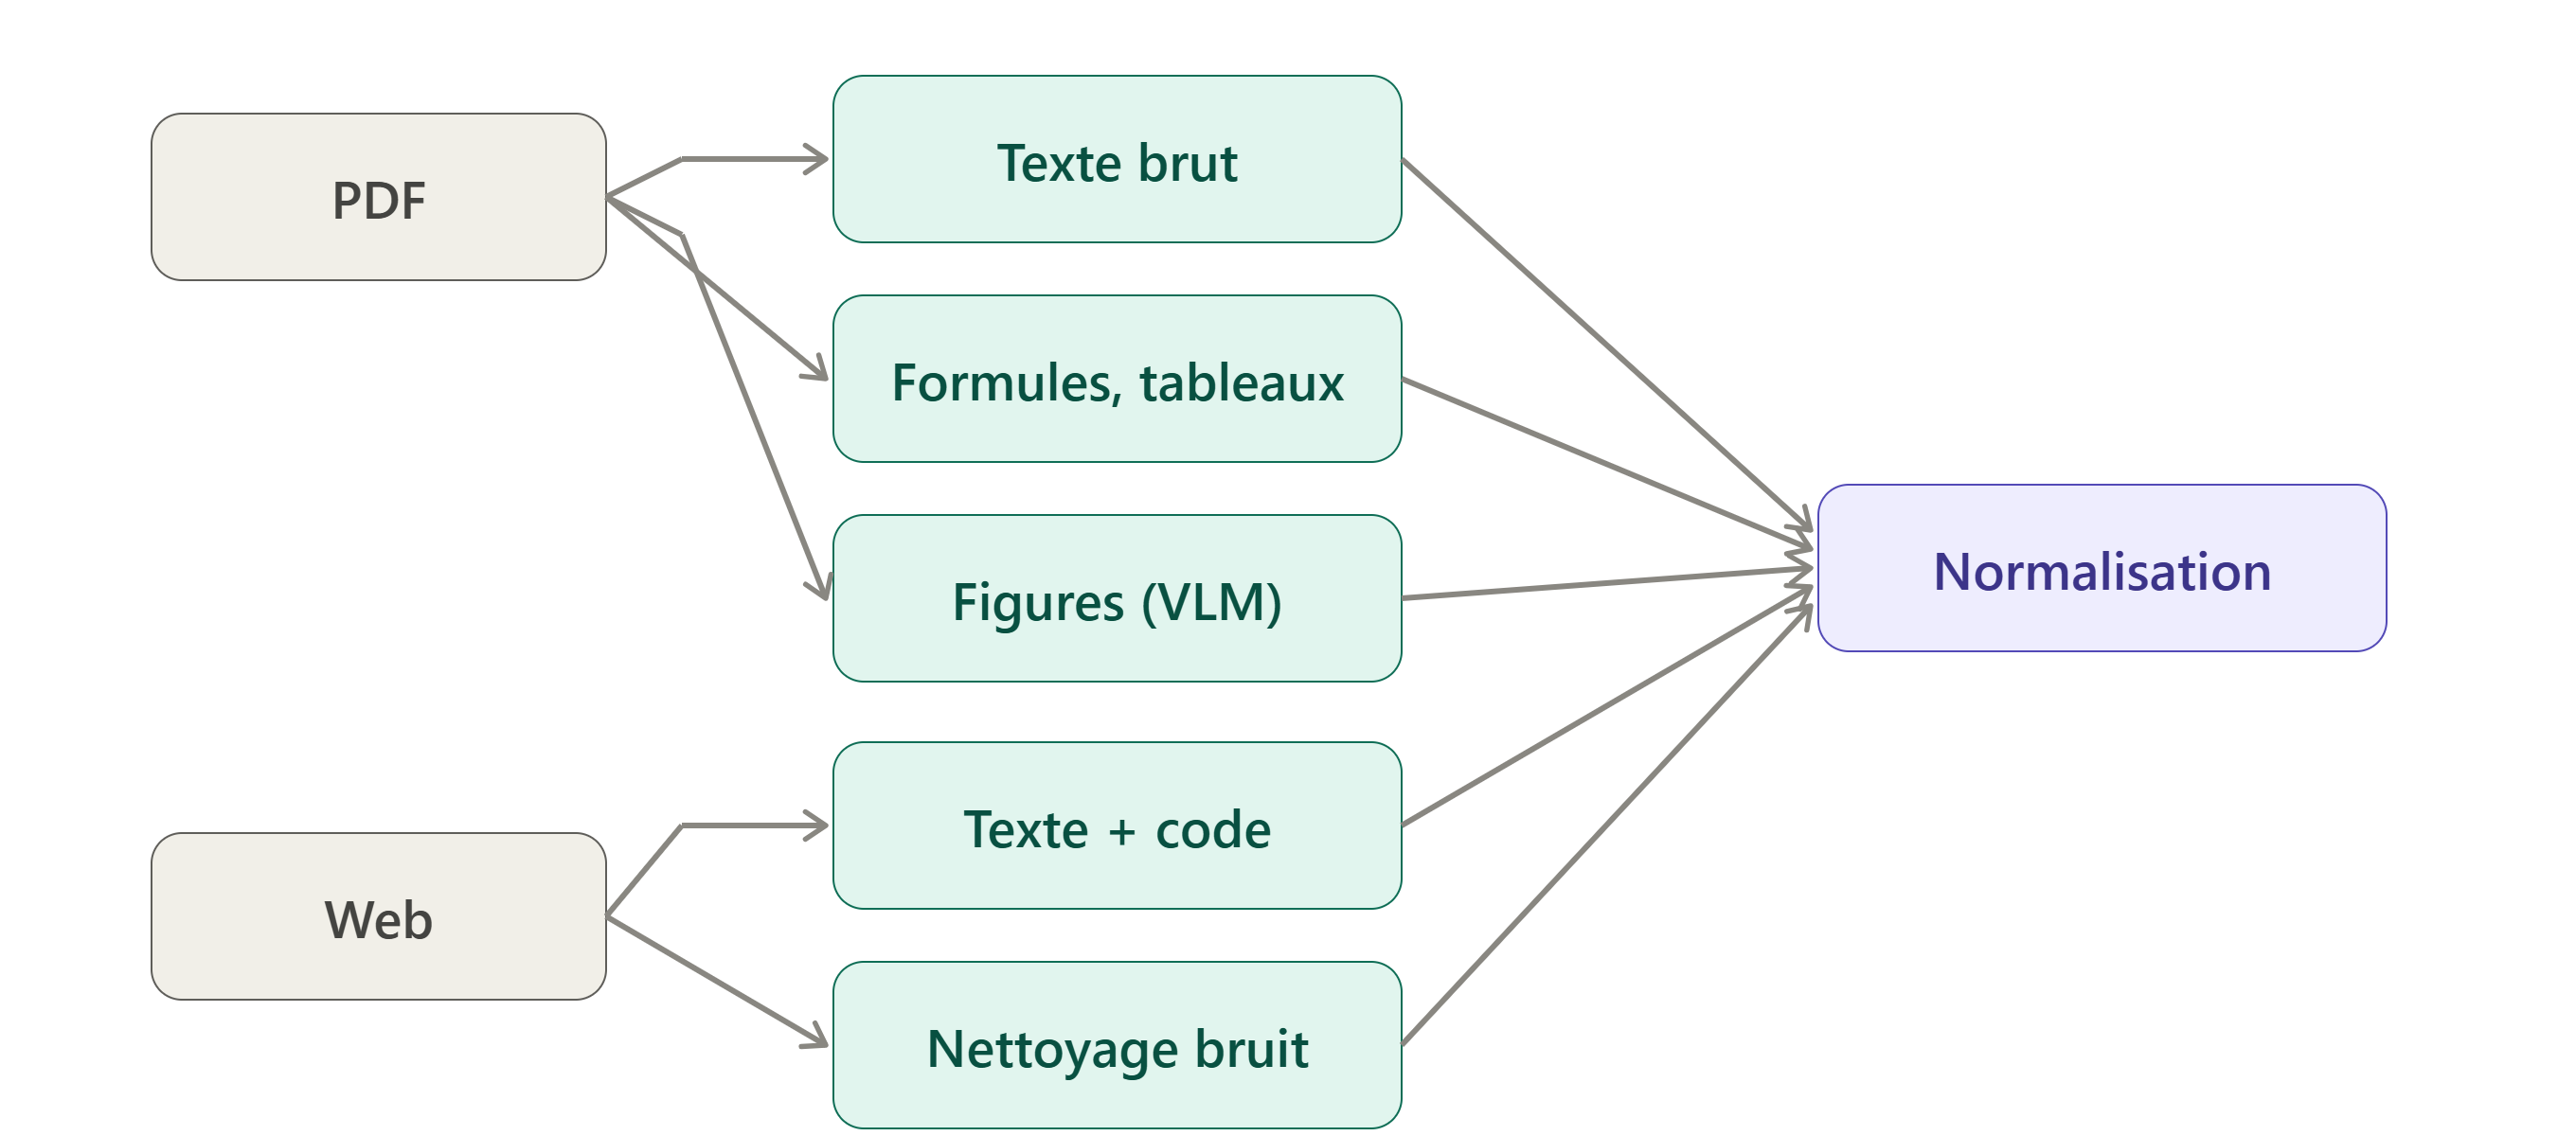
\includegraphics[width=\linewidth]{images/flux_extraction_donnees.png}
\caption{Flux d'extraction des données.}
\label{fig:flux-extraction}
\end{figure}

\subsubsection{Conception de l'ingestion}

Une fois les documents normalisés, l'ingestion les prépare pour la recherche. Le découpage doit concilier deux besoins a priori contradictoires~: des unités suffisamment fines pour permettre une recherche précise, et un contexte suffisamment large pour ne pas fragmenter le sens. Ce compromis structure le choix de stratégie de découpage, détaillé dans la partie Implémentation.

\begin{figure}[H]
\centering
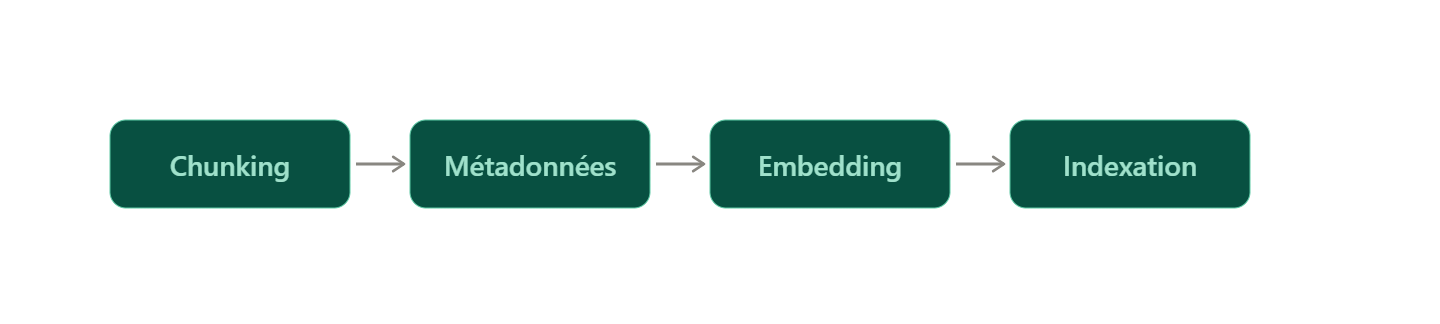
\includegraphics[width=\linewidth]{images/ingestion.png}
\caption{Flux d'ingestion.}
\label{fig:flux-ingestion}
\end{figure}

Chaque unité est ensuite enrichie de métadonnées (document source, type de contenu, position), qui remplissent un double rôle~: permettre la citation précise des sources dans les réponses générées, et filtrer la recherche selon des critères contextuels. Les unités enrichies sont enfin transformées en représentations vectorielles, puis stockées dans une base indexée.

\subsubsection{Conception du \textit{retrieval}}

La recherche doit concilier deux principes de correspondance aux forces complémentaires~: une correspondance lexicale, précise sur les termes exacts (vocabulaire technique, notations mathématiques) mais aveugle aux reformulations, et une correspondance sémantique, qui capte le sens général mais peut manquer une correspondance exacte importante. La façon de combiner ces deux principes est détaillée dans la partie Implémentation.

Une première recherche, optimisée pour parcourir rapidement l'ensemble du corpus, ne garantit pas nécessairement un ordre de pertinence fin parmi les résultats obtenus~: une étape de réévaluation, appliquée aux meilleurs candidats déjà identifiés, permet d'affiner ce classement. Enfin, les passages retenus remontent vers leur parent~: la stratégie parent-enfant restitue le contexte complet des sections pertinentes à la génération.

\begin{figure}[H]
\centering
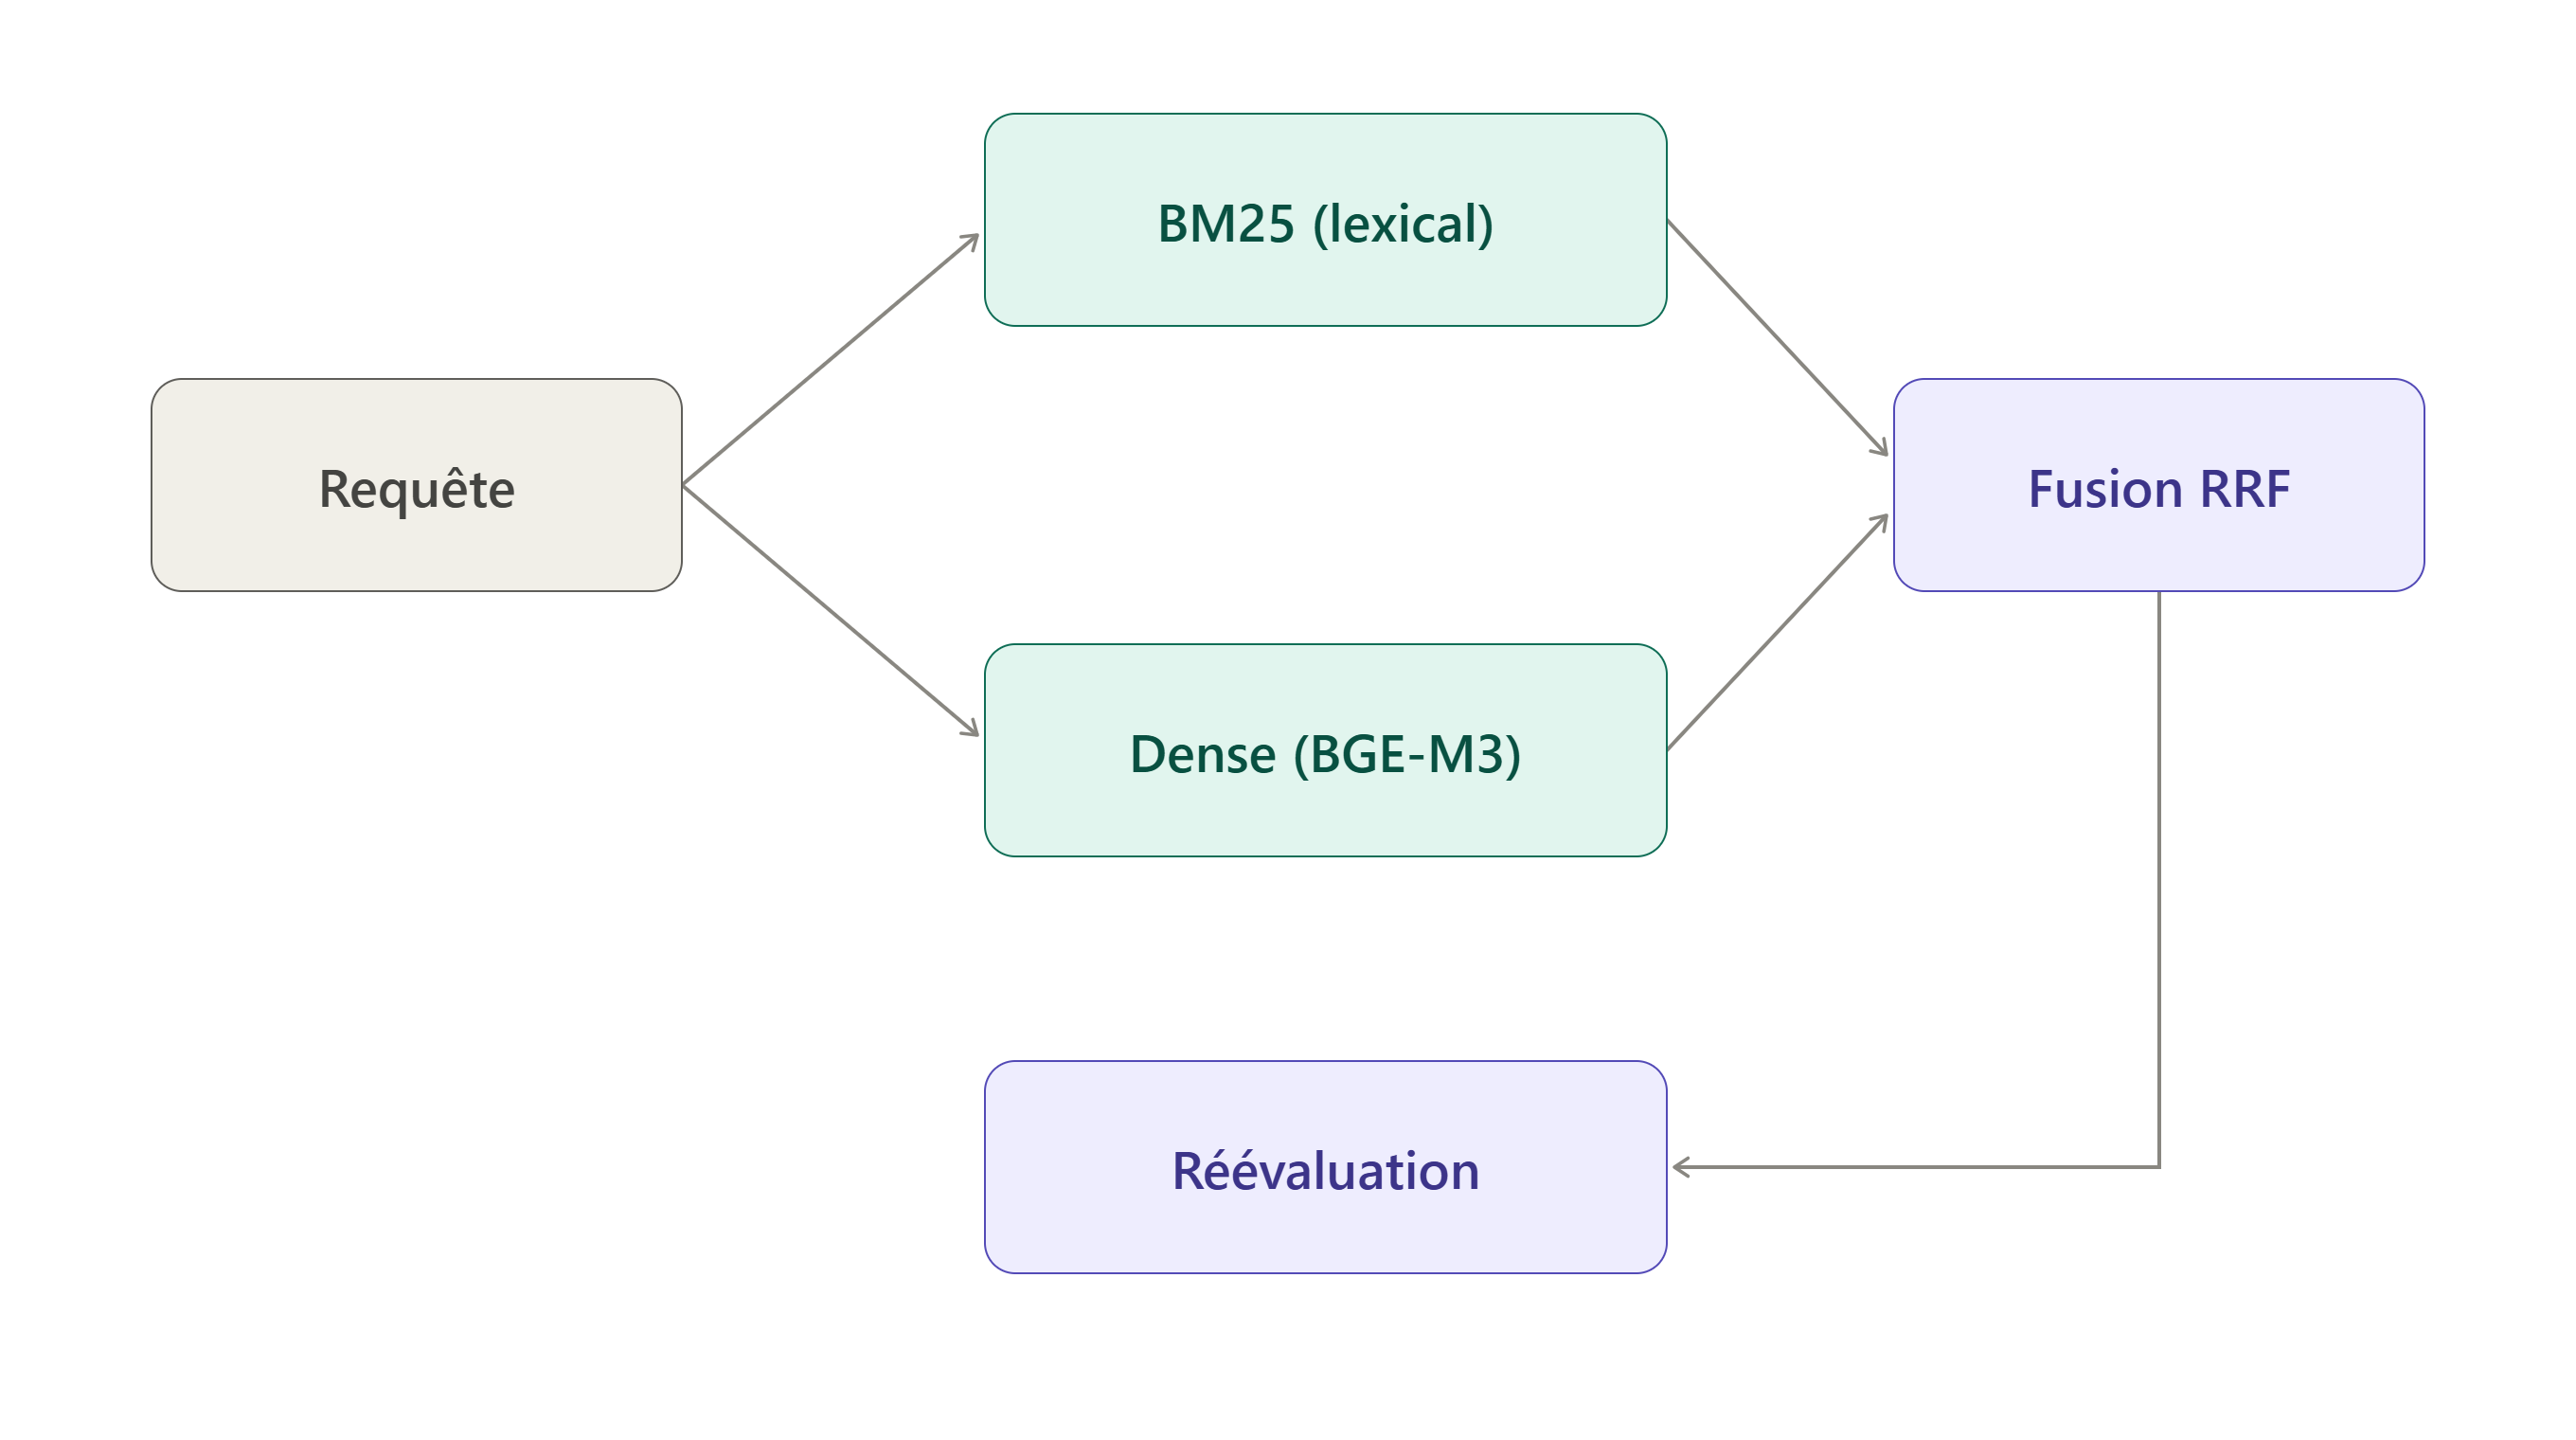
\includegraphics[width=\linewidth]{images/retrieval_cycle.png}
\caption{Flux conceptuel du \textit{retrieval}.}
\label{fig:flux-retrieval}
\end{figure}

\subsubsection{Conception de la génération}

Le contexte récupéré est fourni au modèle de langage aux côtés de la requête de l'utilisateur, encadré par une consigne stricte~: la réponse doit s'appuyer exclusivement sur le contexte fourni, avec un refus explicite en l'absence d'information pertinente. En amont, un module de \textit{query processing} reformule et décompose la question avant la recherche.

\subsection{Implémentation}

\subsubsection{Extraction --- PDF}

Le pipeline PDF repose entièrement sur GLM-OCR pour l'extraction~: le texte, les tableaux, et les figures (détectées et rognées automatiquement) sont produits directement en sortie, sous la forme d'un fichier Markdown, de fichiers JSON structurés, et des images de figures isolées.

Le travail restant porte sur l'interprétation de ces figures et la constitution du document final. Certaines figures repérées par GLM-OCR se sont révélées composites --- plusieurs sous-figures regroupées sous une même figure détectée --- ce qui a nécessité deux logiques de \textit{prompt} distinctes pour le VLM (Qwen3-VL-8B)~: lorsqu'une figure contient des sous-figures, l'ensemble est transmis simultanément au VLM afin d'obtenir une interprétation cohérente de la figure complète~; pour une figure simple, un \textit{prompt} dédié produit directement son interprétation.

Le fichier Markdown final est ensuite constitué en insérant les interprétations produites par le VLM aux emplacements correspondants du texte extrait par GLM-OCR.

\subsubsection{Extraction --- Web}

L'extraction web repose sur un pipeline personnalisé~: un \textit{scraper} convertit le contenu HTML en Markdown, un \textit{crawler} parcourt l'ensemble des pages pertinentes du site ciblé, et un nettoyeur applique un ensemble de traitements sur le Markdown produit --- suppression des balises de mise en forme non porteuses de sens, remplacement des images par des espaces réservés, normalisation des délimiteurs de formules mathématiques vers un format unique, et exclusion automatique des sections d'exercices. Les blocs de code et les formules mathématiques sont conservés tels quels lors de ce nettoyage.

\subsubsection{\textit{Chunking} parent-enfant}

La stratégie retenue est un découpage parent-enfant. Chaque document normalisé est d'abord segmenté en unités parents --- de taille plus large, correspondant à une section cohérente du document. Chaque parent est ensuite subdivisé en unités enfants, plus courtes, calibrées pour la précision de la recherche.

Ce sont les \textit{chunks} enfants qui sont indexés et interrogés lors du \textit{retrieval}. Lorsqu'un enfant est jugé pertinent pour une requête, le système ne retourne pas ce fragment court isolé, mais remonte à son parent associé, transmis à la génération. Le mécanisme découple ainsi la granularité de la recherche (fine, sur les enfants) de la granularité du contexte fourni au modèle (large, via les parents).

\begin{figure}[H]
\centering
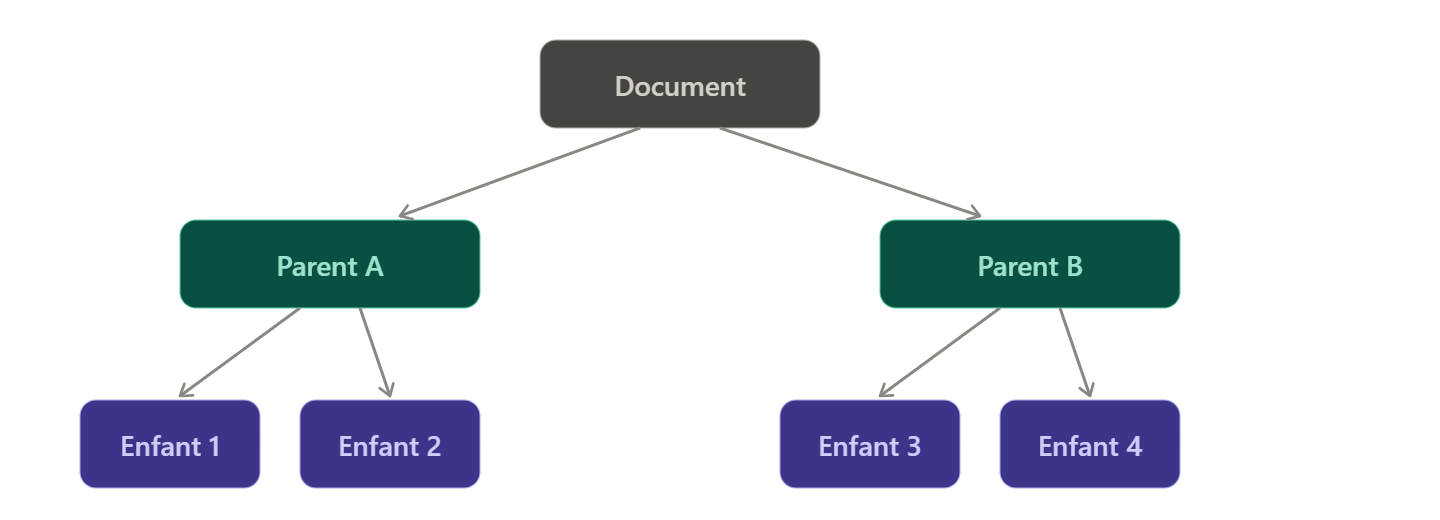
\includegraphics[width=0.85\linewidth]{images/parent-child-chunking.png}
\caption{\textit{Chunking} parent-enfant.}
\label{fig:chunking}
\end{figure}

\subsubsection{Enrichissement par métadonnées}

Chaque \textit{chunk} enfant est associé à un ensemble de métadonnées lors de l'indexation~: le document source dont il est issu, le type de contenu (texte, formule, figure interprétée, code), et sa position dans le document. Le \textit{chunk} parent associé est lui-même référencé comme métadonnée du \textit{chunk} enfant.

Ces métadonnées remplissent deux rôles distincts. Le premier est la citation~: une réponse générée peut être associée précisément au document et à la section d'où provient l'information. Le second est le filtrage~: la recherche peut être restreinte selon un critère de métadonnée, ce qui affine les résultats avant même l'étape de recherche par similarité.

\subsubsection{\textit{Embedding} et indexation}

Les \textit{chunks} enrichis de métadonnées sont vectorisés avec BGE-M3, puis les vecteurs obtenus sont stockés dans ChromaDB, prêts à être interrogés lors du \textit{retrieval}.

\begin{figure}[H]
\centering
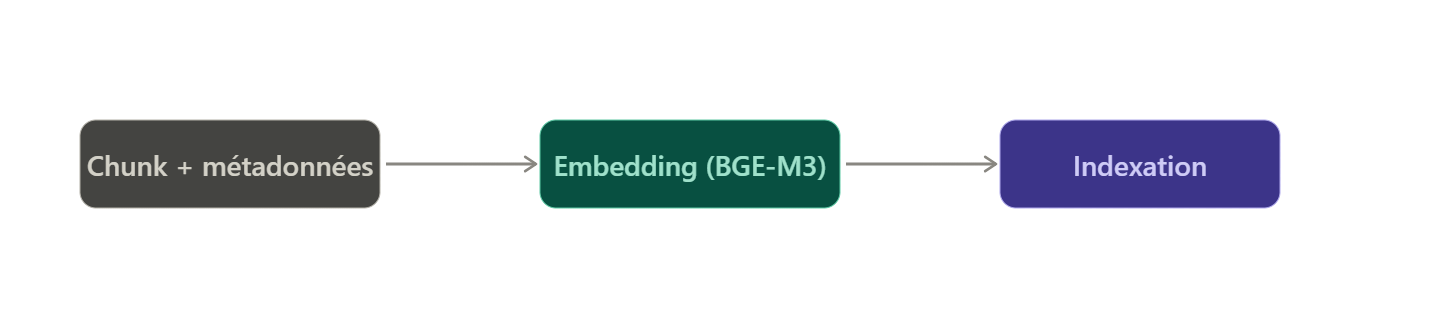
\includegraphics[width=\linewidth]{images/embedding.png}
\caption{Flux d'\textit{embedding} et d'indexation.}
\label{fig:embedding-indexation}
\end{figure}

\subsubsection{\textit{Retrieval} hybride}

La requête de l'utilisateur est transmise simultanément à une recherche lexicale via BM25 et à une recherche dense par similarité vectorielle sur les \textit{embeddings} BGE-M3 indexés dans ChromaDB~; les deux classements obtenus sont combinés par fusion de rang réciproque pondérée (\textit{Weighted RRF}), avec un coefficient $\alpha=0,6$ favorisant légèrement la recherche dense. Le score RRF pondéré d'un document~$d$ est~:
\begin{equation}
  \text{RRF}_w(d) = \frac{\alpha}{k + \operatorname{rang}_{\text{dense}}(d)} + \frac{1-\alpha}{k + \operatorname{rang}_{\text{BM25}}(d)}
  \label{eq:rrf-weighted}
\end{equation}
où $k=60$ est la constante de lissage standard~\cite{cormack2009rrf}. Cette pondération s'appuie sur la position de chaque \textit{chunk} dans chacun des classements plutôt que sur des scores bruts non directement comparables entre eux, tout en donnant un avantage calibré au signal sémantique.

Le classement fusionné est ensuite réévalué par un \textit{cross-encoder}, qui recalcule un score de pertinence en comparant directement la requête et le contenu de chaque candidat --- une réévaluation plus coûteuse mais appliquée uniquement aux meilleurs candidats déjà identifiés par la fusion RRF.

Enfin, les passages retenus après réévaluation remontent vers leurs parents~: la stratégie parent-enfant restitue le contexte complet des sections pertinentes à la génération.

\begin{figure}[H]
\centering
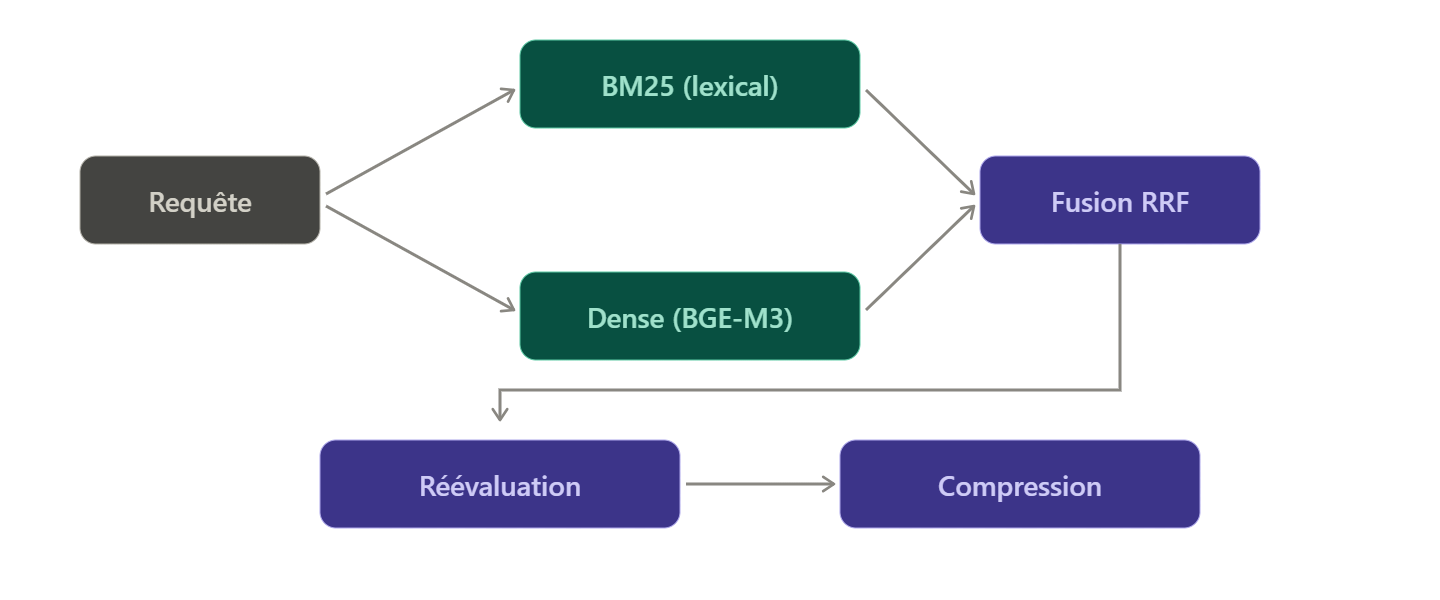
\includegraphics[width=\linewidth]{images/retrieval-sycle.png}
\caption{Pipeline complet de \textit{retrieval}.}
\label{fig:pipeline-retrieval}
\end{figure}

\subsubsection{Génération pédagogique}

Le contexte parent (section complète du document source) est transmis au modèle de langage (Qwen2.5 via Ollama) aux côtés de la requête de l'utilisateur, encadré par un \textit{prompt} de génération qui combine deux exigences. La première est un \textit{grounding} strict~: la réponse doit s'appuyer exclusivement sur le contexte fourni, avec un refus explicite en l'absence d'information pertinente. La seconde donne au système une posture de tuteur~: le \textit{prompt} oriente vers une explication pédagogique adaptée au contenu du cours, favorisant la compréhension du raisonnement sous-jacent plutôt que la seule restitution d'une information.

En amont de la recherche, un module de \textit{query processing} reformule la question de l'étudiant et la décompose en sous-questions indépendantes lorsqu'elle porte sur plusieurs notions distinctes~; chaque sous-question est ensuite recherchée séparément, puis les résultats sont fusionnés avant génération.

\begin{figure}[H]
\centering
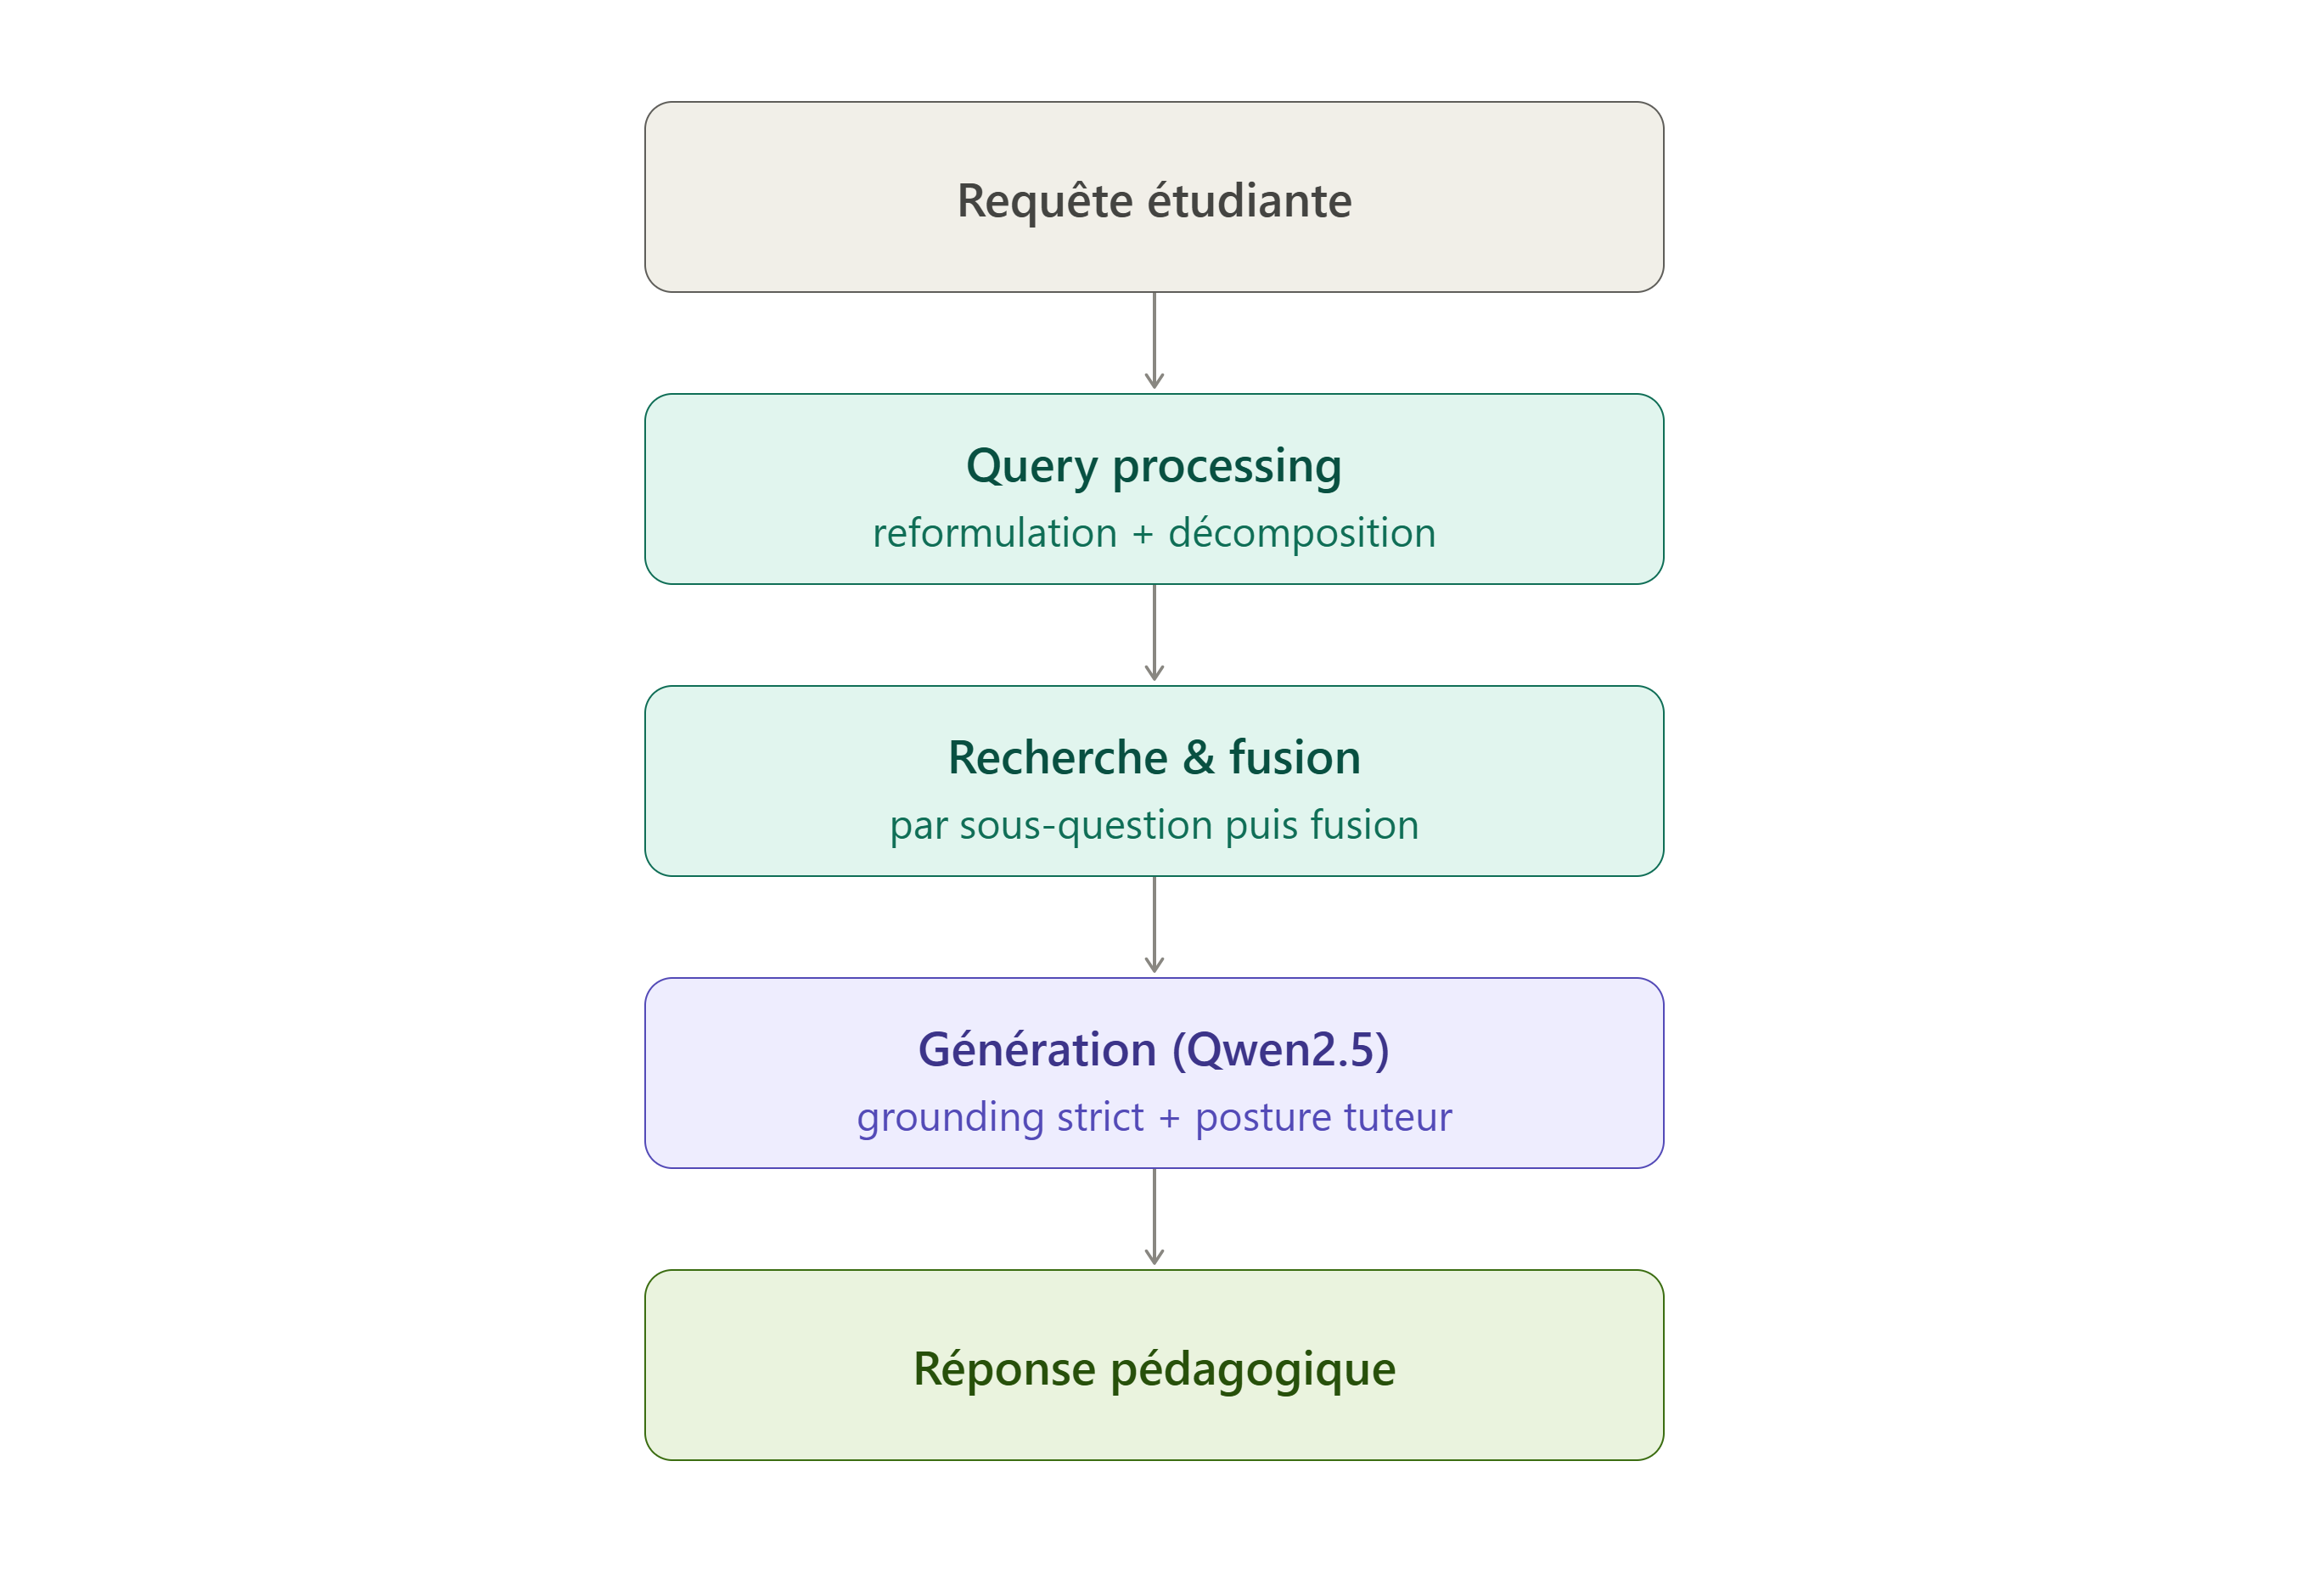
\includegraphics[width=\textwidth]{images/generation_flow.png}
\caption{Flux de génération pédagogique~: de la question utilisateur à la réponse contextualisée.}
\label{fig:generation-flow}
\end{figure}

\subsubsection{Mécanismes de refus}

Deux mécanismes de refus complémentaires encadrent la génération~:

\textbf{Mécanisme 1 — Refus pré-génération par score du \textit{cross-encoder}} (\texttt{should\_refuse\_reranker})~: avant d'appeler le LLM, le score du meilleur passage récupéré (logit du \textit{cross-encoder}) est comparé à un seuil calibré empiriquement (\texttt{RERANKER\_REFUSAL\_THRESHOLD = 0,1119}, cf.~Section~\ref{sec:calibration}). Si le score est inférieur au seuil, le système refuse sans appeler le LLM, économisant un appel de génération.

\textbf{Mécanisme 2 — Refus post-génération par juge LLM} (\texttt{verify\_answer})~: après la génération, un second LLM (Qwen3~:8B) audite la réponse produite. Il vérifie que chaque affirmation est ancrée dans le contexte fourni, sans ajout d'information provenant de la mémoire paramétrique du modèle de génération. Si une information hors-contexte est détectée, la réponse est remplacée par le message de refus. Ce mécanisme s'inspire du paradigme \textit{Self-RAG}~\cite{singh2025agenticrag} tout en utilisant un modèle séparé pour éviter l'auto-évaluation biaisée.

\begin{figure}[H]
\centering
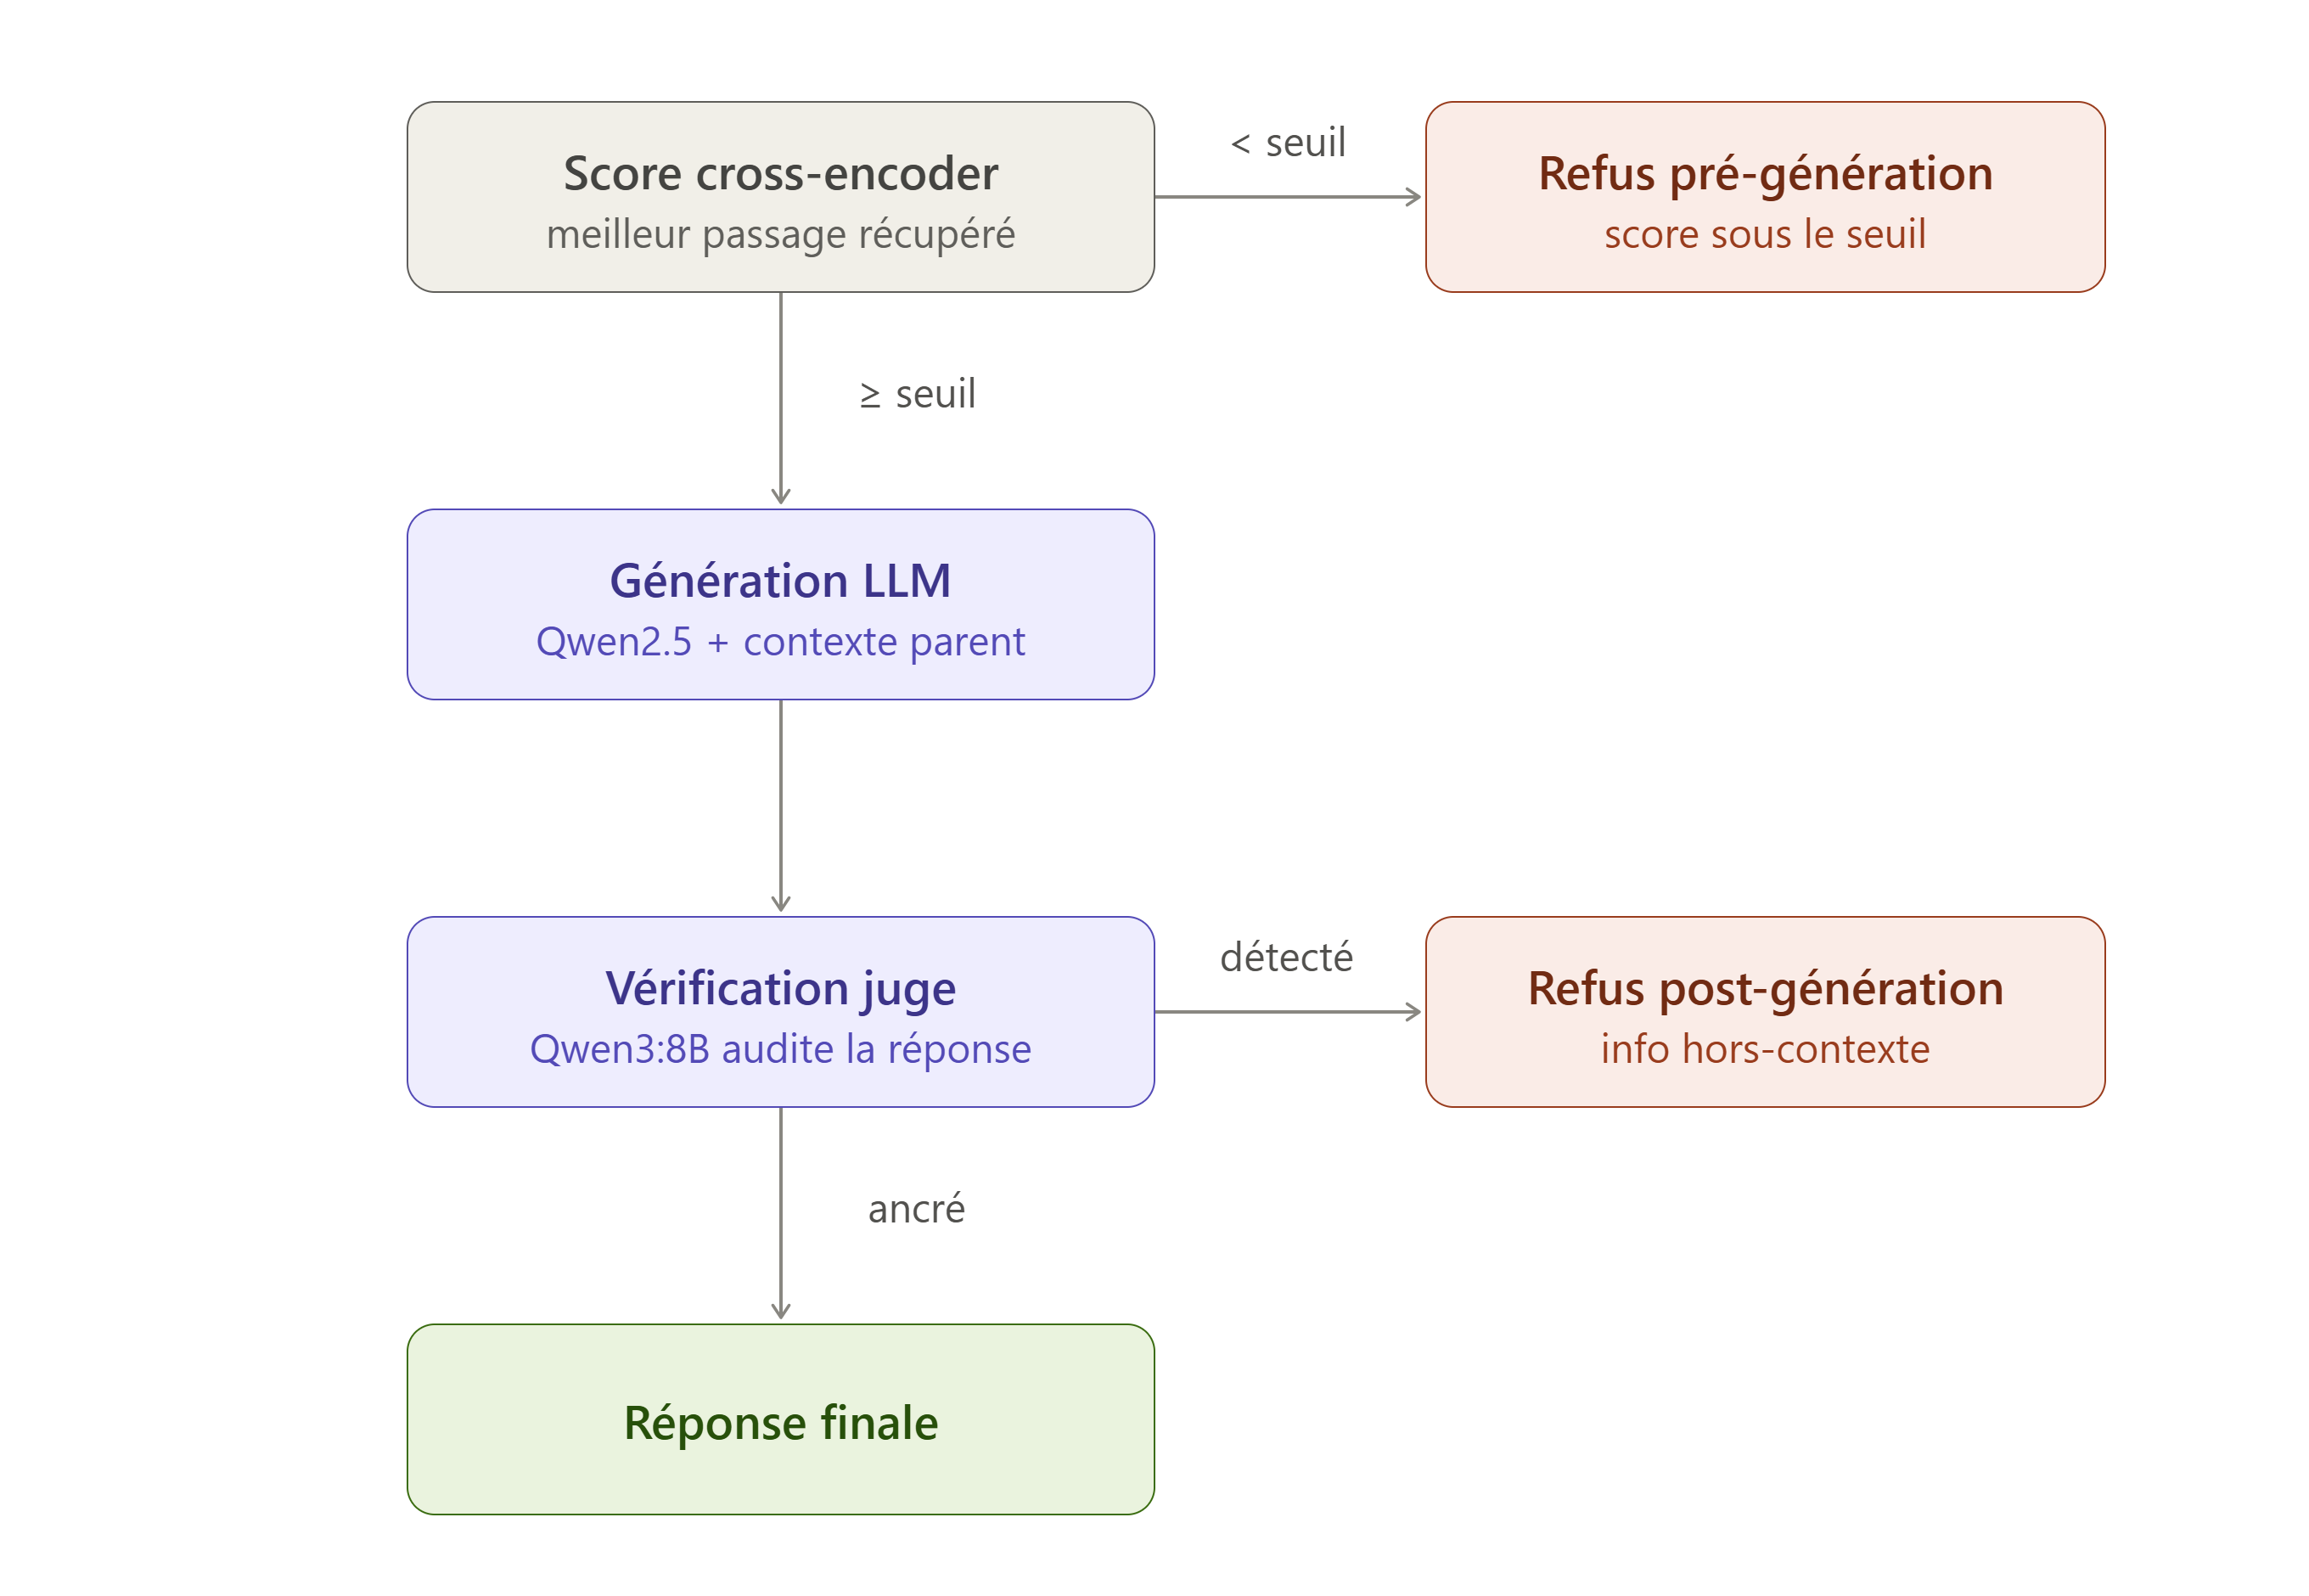
\includegraphics[width=\textwidth]{images/refusal_mechanisms.png}
\caption{Double mécanisme de refus~: refus pré-génération par score du \textit{cross-encoder} (M1) et refus post-génération par juge LLM (M2).}
\label{fig:refusal-mechanisms}
\end{figure}

\subsubsection{Interface en ligne de commande (CLI)}

Le CLI constitue le point d'entrée du système~: l'utilisateur y saisit sa question en texte libre, qui déclenche l'exécution complète de la phase d'exécution du pipeline, et reçoit en sortie la réponse générée accompagnée des sources citées.

Le CLI sert également d'interface pour l'évaluation par lots~: il accepte un jeu de questions en entrée (le \textit{golden dataset}) et produit en sortie l'ensemble des réponses correspondantes.

\begin{figure}[H]
\centering
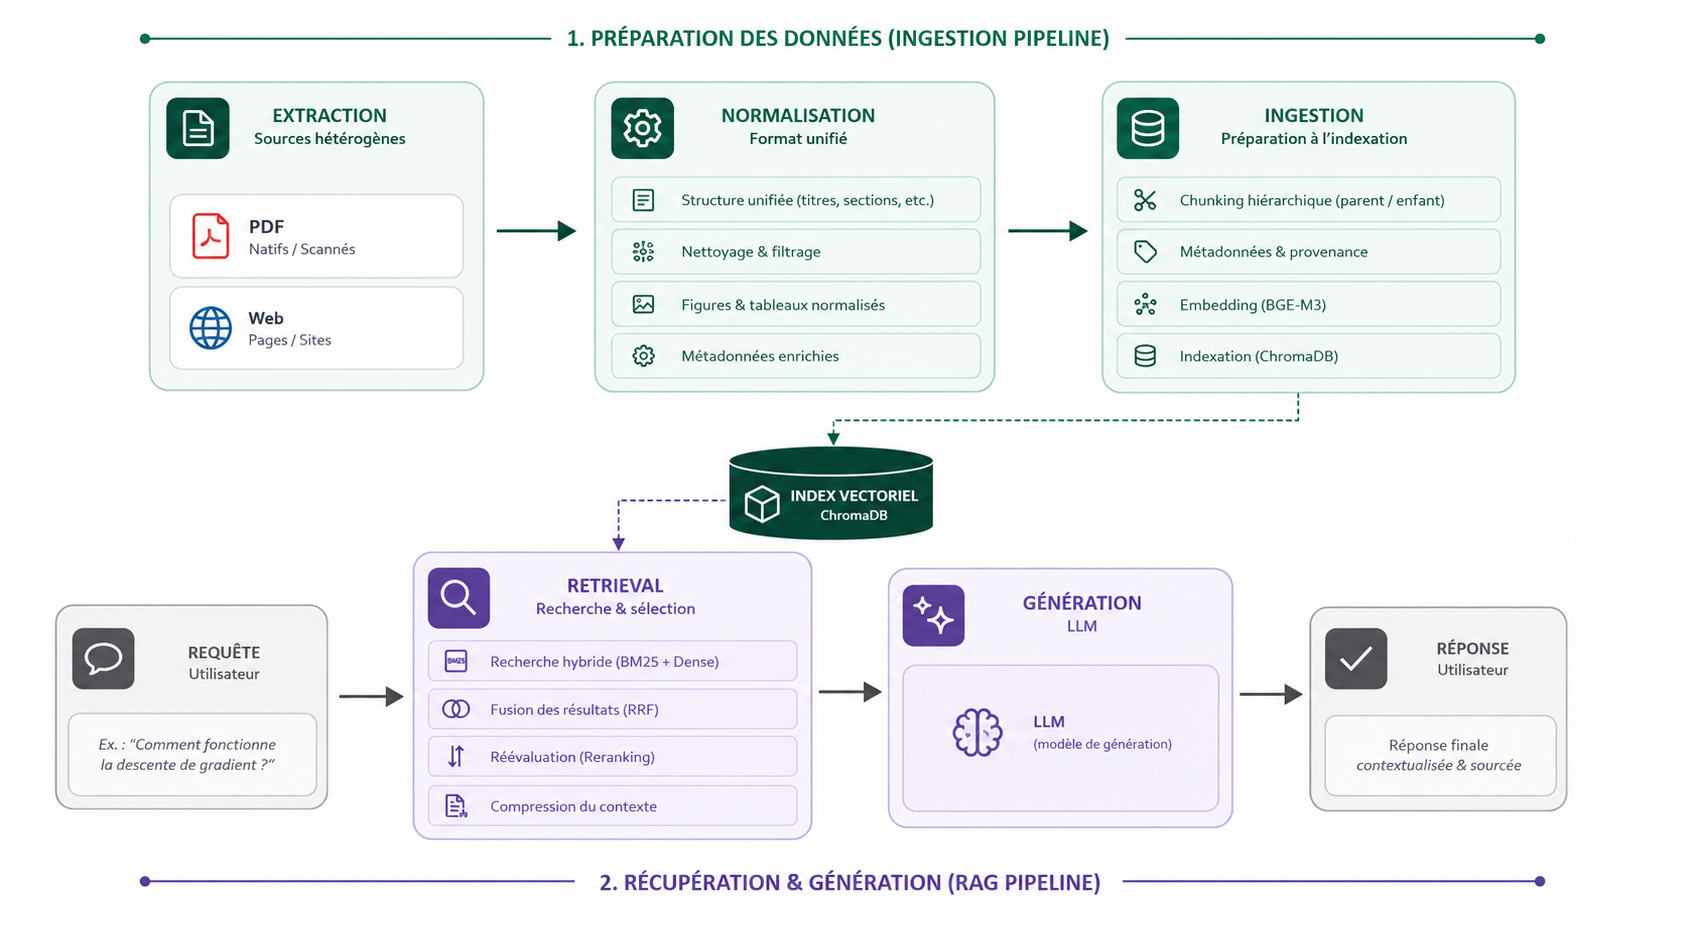
\includegraphics[width=\linewidth]{images/final-architecture.png}
\caption{Flux global détaillé du projet. Préparation (extraction PDF/Web, normalisation, ingestion) puis exécution (CLI $\to$ \textit{retrieval} $\to$ génération $\to$ réponse).}
\label{fig:flux-global}
\end{figure}

% =============================================================
%             CHAPITRE 6 : ÉVALUATION
% =============================================================
\section{Évaluation}
\label{sec:evaluation}

L'évaluation du système vise à répondre à trois questions~: (i)~le système retrouve-t-il les passages pertinents du corpus pour une question donnée~? (ii)~la réponse générée est-elle fidèle au contexte récupéré~? (iii)~le système sait-il refuser de répondre lorsque l'information n'est pas présente dans le corpus~? Cette section décrit le protocole expérimental et présente les résultats obtenus.

\subsection{Protocole expérimental}

\subsubsection{Constitution du jeu de données de référence}

Un jeu de données de référence (\textit{golden dataset}) a été constitué en utilisant le synthétiseur de DeepEval~\cite{deepeval2024} pour générer automatiquement des paires question--réponse à partir du corpus indexé. Contrairement à une approche naïve où DeepEval appliquerait son propre \textit{chunking} (taille 800, pas de parent-enfant), le protocole adopté garantit l'alignement entre le \textit{chunking} du jeu de données et celui du système réel~:

\begin{enumerate}
  \item Le corpus est d'abord découpé avec \textbf{notre} chunker parent-enfant (1775~parents, 8379~enfants).
  \item Chaque parent est exporté dans un fichier Markdown individuel dans un dossier dédié (\texttt{parents\_cours\_ml/}). Le fichier contient le texte complet de la section parent et un en-tête YAML avec ses métadonnées (source, numéro de section, pages). Cette étape est réalisée par \texttt{scripts101/generate\_golden\_dataset.py}.
  \item DeepEval est configuré avec une taille de \textit{chunk} de 100\,000~caractères (bien supérieure à la taille maximale d'un parent, $\sim$80\,000), garantissant qu'\textit{aucun re-chunking} n'est appliqué~: chaque fichier devient un unique \textit{chunk} DeepEval = exactement un parent.
  \item Les \textit{contextes de référence} (\textit{gold contexts}) produits sont donc exactement nos parents réels, assurant un alignement parfait avec le système.
\end{enumerate}

Le jeu de données final comporte \textbf{60~questions} réparties en trois catégories~:
\begin{itemize}
  \item \textbf{20 questions \textit{single passage}}~: réponse contenue dans un seul parent. Teste la qualité de la génération pure.
  \item \textbf{20 questions \textit{multi passage}}~: réponse nécessitant 2--3 parents de sources différentes. Teste la capacité de \textit{retrieval} et de synthèse.
  \item \textbf{20 questions sans réponse} (\textit{unanswerable})~: question plausible mais dont la réponse n'est pas présente dans le contexte fourni. Teste le mécanisme de refus.
\end{itemize}

Les 60~questions sont réparties en un jeu de calibration (15~questions : 10~answerable + 5~unanswerable) et un jeu de test (45~questions : 30~answerable + 15~unanswerable).

\textbf{Correction du biais du dataset.} Lors des premières évaluations, nous avons constaté un problème méthodologique~: le synthétiseur de DeepEval génère les questions \textit{unanswerable} en sélectionnant un \textit{chunk} du corpus, puis en formulant une question dont la réponse est absente de \textit{ce chunk spécifique} --- mais potentiellement présente ailleurs dans le corpus. Comme l'ensemble du corpus porte sur le machine learning, les questions générées restaient dans le domaine du ML et le système pouvait légitimement y répondre via le \textit{retrieval} d'autres passages du corpus. La métrique de refus était donc non informative (0\,\% de refus détectés sur les 15~questions), non pas en raison d'une défaillance du mécanisme de refus, mais parce que les questions étaient \textit{de facto} répondables. Nous avons donc remplacé ces 15~questions par des questions de domaines totalement étrangers au \textit{Deep Learning} (géographie, biologie, histoire, informatique hors-ML, physique, chimie, économie).

\subsubsection{Métriques d'évaluation}

L'évaluation combine des métriques de \textit{retrieval} et de refus.

\paragraph{Métriques de \textit{retrieval}}

\begin{itemize}
  \item \textbf{Hit@4}~: proportion de questions pour lesquelles au moins un passage pertinent figure parmi les 4~premiers résultats.
  \item \textbf{MRR} (\textit{Mean Reciprocal Rank})~: moyenne de l'inverse du rang du premier passage pertinent.
  \item \textbf{nDCG@4} (\textit{Normalized Discounted Cumulative Gain})~: pertinence graduée du top-4, avec scores de chevauchement lexical bidirectionnel.
  \item \textbf{Precision@4}~: proportion de passages pertinents parmi les 4~premiers résultats.
\end{itemize}

\paragraph{Métriques de refus}

\begin{itemize}
  \item \textbf{Refusal Correctness}~: proportion de décisions de refus correctes (refuser une question sans réponse, répondre à une question avec réponse).
  \item \textbf{Refusal Precision / Recall / F1}~: précision (un refus est-il justifié~?), rappel (toutes les questions sans réponse sont-elles refusées~?), et leur moyenne harmonique.
\end{itemize}

\subsection{Calibration du mécanisme de refus}
\label{sec:calibration}

Le mécanisme de refus pré-génération (M1) repose sur le score du \textit{cross-encoder} (\texttt{hits[0]["dist"]}). Pour déterminer le seuil optimal, nous avons collecté les scores du \textit{cross-encoder} sur le jeu de test complet (30~questions answerable + 15~questions unanswerable hors-domaine), en mode \texttt{hybrid\_rerank} avec le \textit{refusal gate} désactivé.

\begin{table}[H]
\centering
\small
\begin{tabularx}{\linewidth}{L{3.5cm} C{1.5cm} C{2cm} C{2cm} C{2cm}}
\toprule
\rowcolor{bleuPrincipal}
\textcolor{white}{\textbf{Catégorie}} & \textcolor{white}{\textbf{n}} & \textcolor{white}{\textbf{min}} & \textcolor{white}{\textbf{médiane}} & \textcolor{white}{\textbf{max}} \\
\midrule
Answerable   & 30 & 0,1119 & 0,8184 & 0,9985 \\
Unanswerable & 15 & 0,0006 & 0,0022 & 0,0118 \\
\bottomrule
\end{tabularx}
\caption{Distribution des scores du \textit{cross-encoder} par catégorie.}
\label{tab:calibration-distrib}
\end{table}

Le Tableau~\ref{tab:calibration-distrib} montre une séparation parfaite~: le score maximal des questions \textit{unanswerable} (0,0118) est dix fois inférieur au score minimal des questions \textit{answerable} (0,1119). Il n'existe \textbf{aucun chevauchement} entre les deux distributions. Le seuil optimal, déterminé en maximisant l'exactitude de classification, est de \textbf{0,1119}, pour une \textbf{exactitude de 100\,\%} (15~vrais refus, 0~faux refus, 0~faux non-refus).

Il convient de nuancer ce résultat~: la séparation parfaite est facilitée par le choix de questions \textit{unanswerable} volontairement hors-domaine (géographie, biologie, histoire), que le \textit{cross-encoder} discrimine trivialement du corpus de ML. Sur des questions \textit{near-domain} --- des questions de ML dont le cours ne traite pas, comme \textit{«~Comment fonctionne un Vision Transformer (ViT)~?~»} --- la tâche de discrimination serait significativement plus difficile, les distributions de scores se chevauchant davantage. Ce point est discuté plus en détail dans la Section~\ref{sec:discussion}.

Ce résultat contraste avec la calibration initiale sur les questions DeepEval, où les distributions se chevauchaient fortement (médianes 0,680 vs. 0,764, exactitude 68,3\,\%). Le changement de dataset a permis de révéler le véritable pouvoir discriminant du \textit{cross-encoder}.

\begin{figure}[H]
\centering
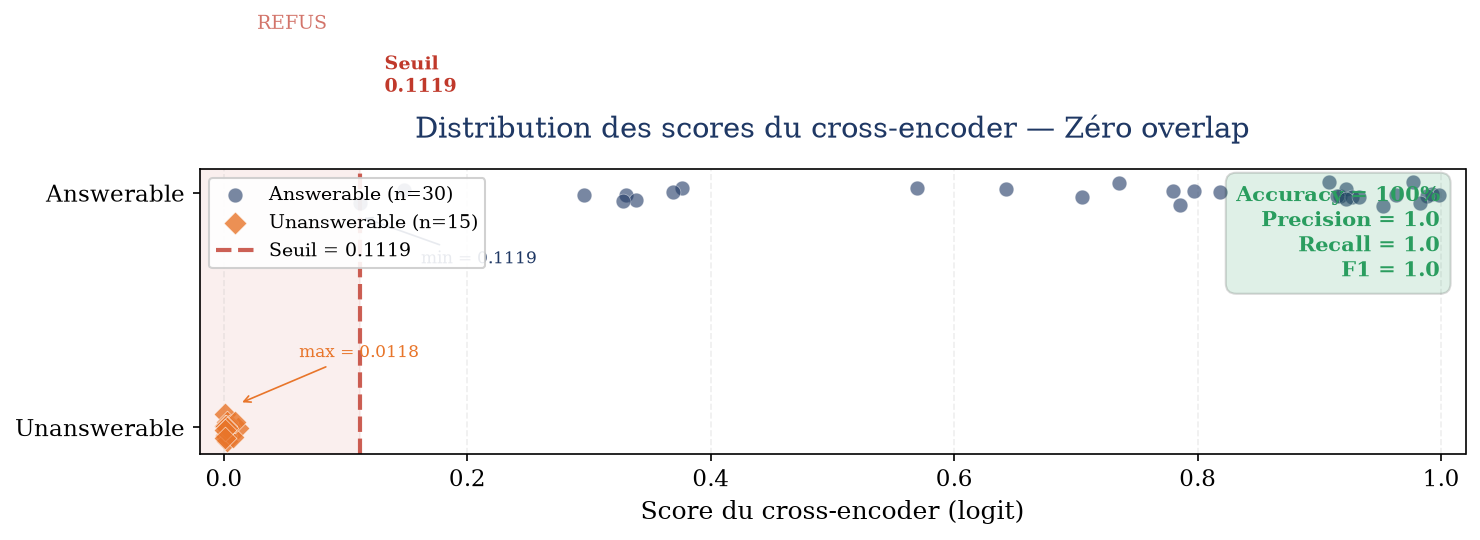
\includegraphics[width=\linewidth]{images/fig2_reranker_distribution.png}
\caption{Distribution des scores du \textit{cross-encoder}~: \textit{answerable} (bleu) vs. \textit{unanswerable} (orange). La ligne pointillée rouge marque le seuil calibré (0,1119). L'absence de chevauchement permet une discrimination parfaite.}
\label{fig:calibration}
\end{figure}

\subsection{Étude d'ablation}

Pour mesurer la contribution de chaque composant du pipeline, une étude d'ablation en quatre étapes a été menée sur le jeu de test (45~questions).

\begin{table}[H]
\centering
\small
\begin{tabularx}{\linewidth}{C{1.2cm} L{2.8cm} L{4cm} C{2.2cm} C{2.2cm}}
\toprule
\rowcolor{bleuPrincipal}
\textcolor{white}{\textbf{Étape}} & \textcolor{white}{\textbf{QP}} & \textcolor{white}{\textbf{Retrieval}} & \textcolor{white}{\textbf{RG}} & \textcolor{white}{\textbf{Rôle}} \\
\midrule
1 & ---  & Dense seul (BGE-M3)      & --- & Baseline \\
2 & Oui  & Dense seul (BGE-M3)      & --- & Apport du QP \\
3 & Oui  & Hybride (BM25 + BGE-M3 + RRF) & --- & Apport de l'hybridation \\
4 & Oui  & Hybride + Cross-encoder  & Oui & Système complet \\
\bottomrule
\end{tabularx}
\caption{Configurations des quatre étapes de l'étude d'ablation.}
\label{tab:ablation}
\end{table}

\subsection{Résultats de \textit{retrieval}}


\begin{table}[H]
\centering
\small
\begin{tabularx}{\linewidth}{L{3.2cm} C{2.2cm} C{2.2cm} C{2.2cm} C{2.6cm}}
\toprule
\rowcolor{bleuPrincipal}
\textcolor{white}{\textbf{Métrique}} & \textcolor{white}{\textbf{Baseline}} & \textcolor{white}{\textbf{+ QP}} & \textcolor{white}{\textbf{+ Hybride}} & \textcolor{white}{\textbf{+ Reranker}} \\
\midrule
Hit@4      & 0,900 & 0,900 & 0,900 & \textbf{0,967} \\
MRR        & 0,811 & 0,800 & 0,772 & \textbf{0,867} \\
nDCG@4     & 0,942 & 0,932 & 0,918 & \textbf{0,939} \\
Precision@4& 0,308 & 0,375 & 0,392 & \textbf{0,408} \\
\bottomrule
\end{tabularx}
\caption{Performances de \textit{retrieval} aux quatre étapes de l'ablation (30~questions \textit{answerable}). }
\label{tab:resultats-retrieval}
\end{table}

Le Tableau~\ref{tab:resultats-retrieval} montre que le \textit{cross-encoder} est le composant qui apporte le gain le plus significatif~: +6,7~points de Hit@4 et +5,6~points de MRR par rapport à la baseline. L'hybridation (BM25 + dense) réduit légèrement le nDCG (-2,4~points) et le MRR (-1,1~points) par rapport à l'étape précédente (+QP), un compromis attendu~: la diversité accrue des résultats bénéficie au rappel mais dilue la précision du classement. Le \textit{cross-encoder} corrige ensuite cette dilution (+2,1~points de nDCG et +9,5~points de MRR). Le \textit{query processing} corrigé maintient les performances de la baseline, validant l'efficacité du correctif (cf.~Section~\ref{sec:bug-qp}).

\begin{figure}[H]
\centering
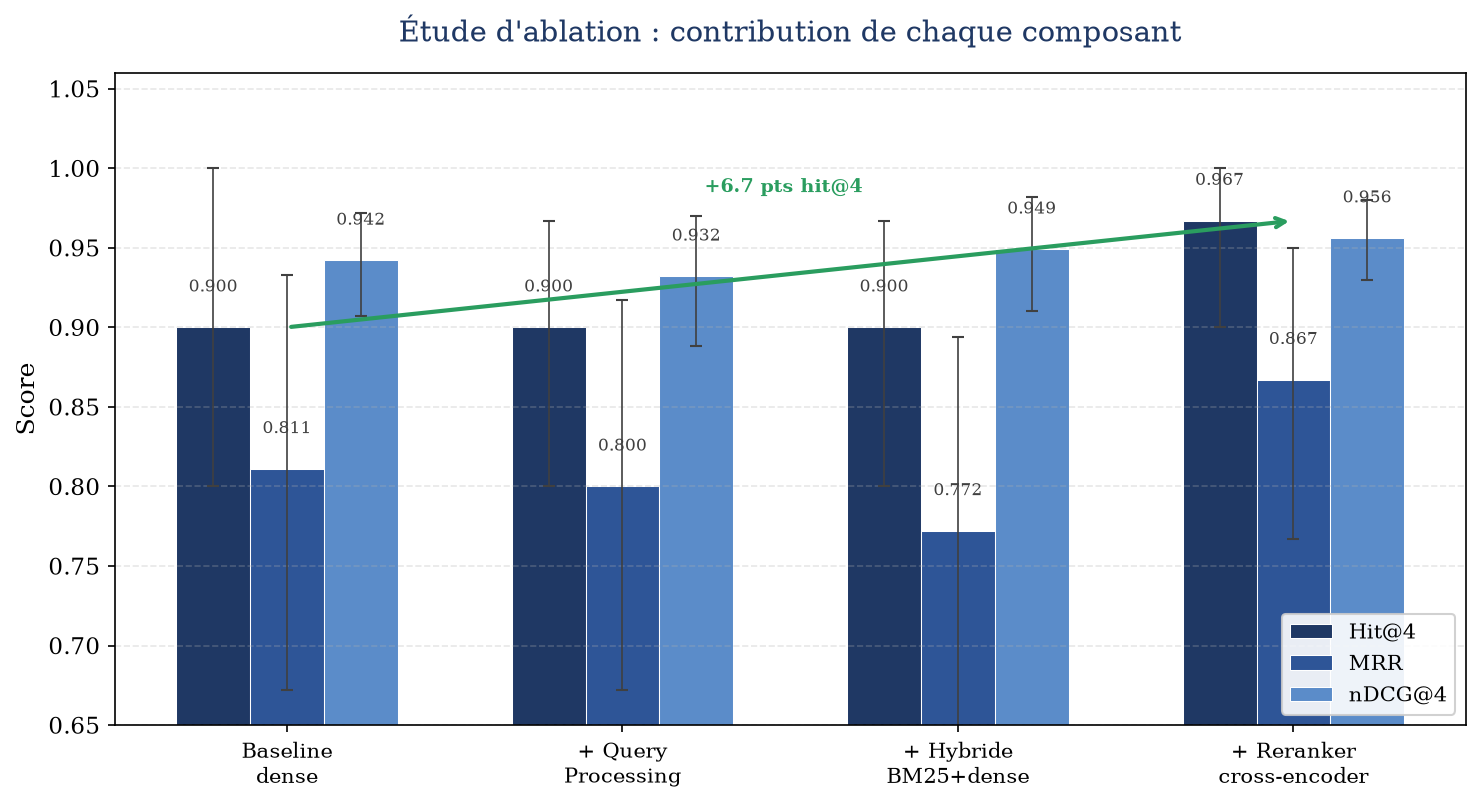
\includegraphics[width=\linewidth]{images/fig1_ablation.png}
\caption{Étude d'ablation~: évolution des métriques de \textit{retrieval} aux quatre étapes.}
\label{fig:ablation}
\end{figure}

\subsection{Résultats par catégorie}

\begin{table}[H]
\centering
\small
\begin{tabularx}{\linewidth}{L{3.2cm} C{3cm} C{3cm} C{3cm}}
\toprule
\rowcolor{bleuPrincipal}
\textcolor{white}{\textbf{Métrique}} & \textcolor{white}{\textbf{Single (15q)}} & \textcolor{white}{\textbf{Multi (15q)}} & \textcolor{white}{\textbf{$\Delta$}} \\
\midrule
Hit@4      & 1,000 [1,000--1,000] & 0,933 [0,800--1,000] & -0,067 \\
MRR        & 0,967 [0,900--1,000] & 0,767 [0,567--0,933] & \textbf{-0,200} \\
nDCG@4     & 0,981 [0,951--0,997] & 0,897 [0,839--0,950] & -0,084 \\
\bottomrule
\end{tabularx}
\caption{Performances par catégorie pour le système complet (hybride + \textit{cross-encoder}).}
\label{tab:categories}
\end{table}

Le Tableau~\ref{tab:categories} confirme que la configuration \textit{single passage} est résolue de manière quasi parfaite (Hit@4~=~1,000, MRR~=~0,967). Le \textit{multi passage} demeure plus exigeant, avec un MRR inférieur de 0,200~point~: la synthèse d'informations issues de plusieurs sources reste un défi pour le \textit{retrieval}, même avec le \textit{cross-encoder}.

\begin{figure}[H]
\centering
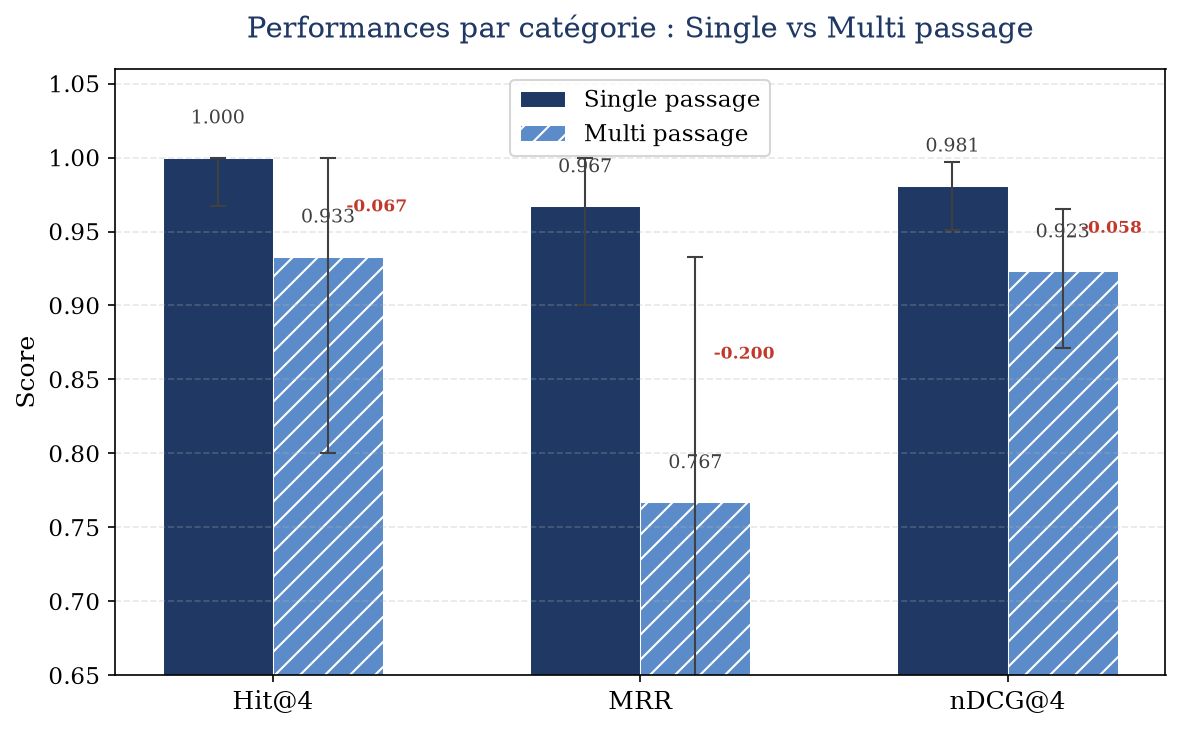
\includegraphics[width=0.85\linewidth]{images/fig3_single_vs_multi.png}
\caption{Comparaison des performances entre les catégories \textit{single} et \textit{multi passage}.}
\label{fig:categories}
\end{figure}

\subsection{Diagnostic et correction du \textit{Query Processing}}
\label{sec:bug-qp}

Lors de l'évaluation de l'étape~2 (ajout du QP), une dégradation inattendue des performances de \textit{retrieval} a été observée~: le Hit@4 chutait de 0,900 à 0,733 (-16,7~points) et le MRR de 0,811 à 0,572 (-23,9~points). Trois causes racines ont été identifiées~:

\begin{enumerate}
  \item \textbf{Question reformulée jetée}~: la requête reformulée (intention globale) était écartée dès que des sous-questions étaient produites, ne laissant que des sous-questions étroites pour le \textit{retrieval}.
  \item \textbf{Tri global par score}~: les scores cosinus des sous-questions étroites étaient artificiellement plus élevés que celui de la question reformulée, poussant les hits pertinents hors du top-4.
  \item \textbf{Fonction de pertinence asymétrique}~: la métrique \texttt{\_is\_relevant()} mesurait uniquement le chevauchement dans le sens \textit{gold}$\to$\textit{hit}, pénalisant les hits courts mais parfaitement pertinents pour une sous-question.
\end{enumerate}

Trois correctifs ont été appliqués~: (i)~toujours inclure la question reformulée dans les requêtes de \textit{retrieval}~; (ii)~remplacer le tri global par score par une fusion \textit{round-robin} qui entrelace les résultats de chaque requête~; (iii)~utiliser un chevauchement bidirectionnel $\max(\text{gold}\to\text{hit}, \text{hit}\to\text{gold})$ avec un seuil abaissé à 0,4.

Après correction, le Hit@4 est remonté à 0,900, identique à la baseline sans QP. L'écart résiduel sur le MRR (-0,011) est acceptable~: le \textit{round-robin} privilégie délibérément la diversité des résultats multi-requêtes au détriment du score pur.

\begin{figure}[H]
\centering
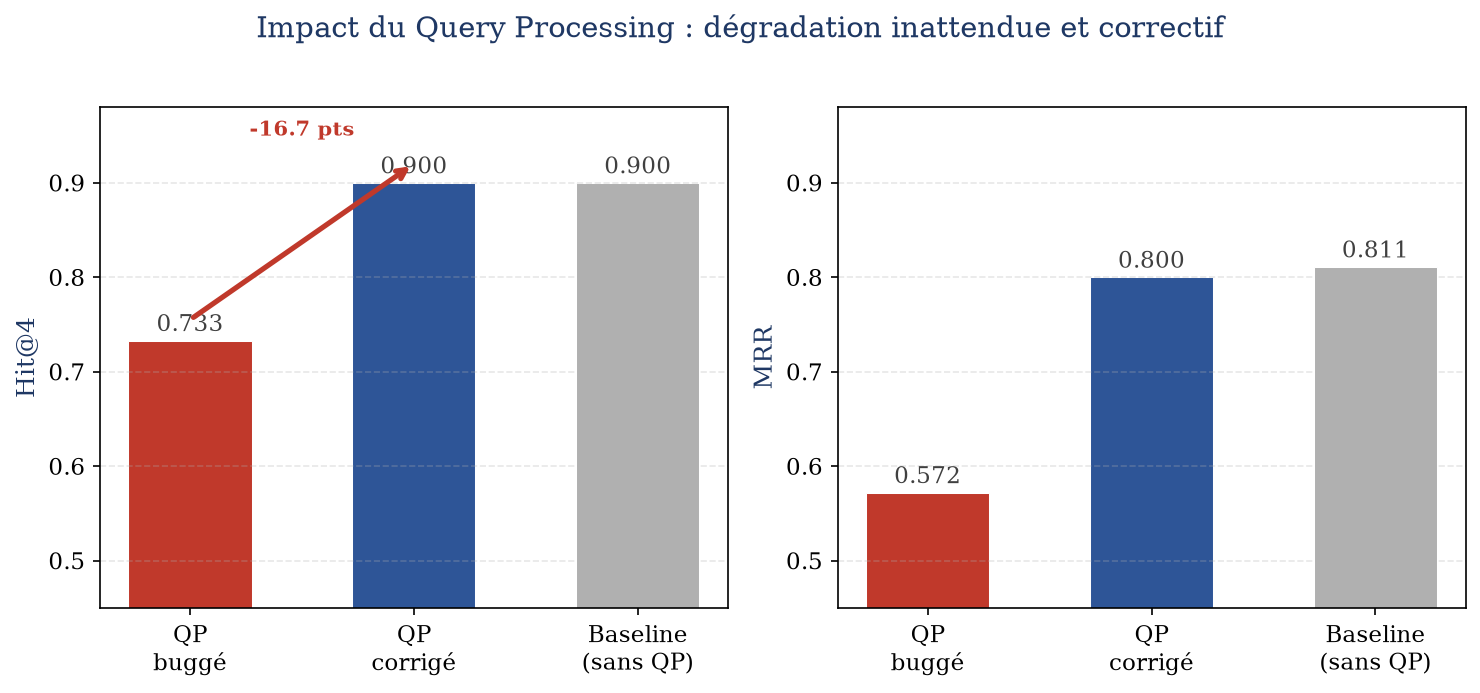
\includegraphics[width=\linewidth]{images/fig4_bug_qp.png}
\caption{Impact du \textit{Query Processing}~: dégradation initiale (-16,7~pts Hit@4) et récupération après correctif.}
\label{fig:bug-qp}
\end{figure}

\subsection{Performances de génération}

La qualité des réponses générées a été évaluée via le \textit{framework} Ragas~\cite{es2024ragas} sur le Run~1 (baseline dense, 30~questions \textit{answerable}), avec Qwen3~:8B comme juge LLM.

\begin{table}[H]
\centering
\small
\begin{tabularx}{\linewidth}{L{5cm} C{3cm}}
\toprule
\rowcolor{bleuPrincipal}
\textcolor{white}{\textbf{Métrique}} & \textcolor{white}{\textbf{Score}} \\
\midrule
Fidélité (\textit{faithfulness})     & 0,887 \\
Précision du contexte (\textit{context precision}) & 0,840 \\
Exactitude factuelle (\textit{custom correctness}, juge 1--5) & 0,786 \\
\bottomrule
\end{tabularx}
\caption{Performances de génération sur les 30~questions \textit{answerable} (Run~1, baseline dense).}
\label{tab:generation}
\end{table}

La fidélité de 0,887 indique que près de 89\,\% des affirmations produites sont ancrées dans le contexte fourni. La précision du contexte de 0,840 confirme que les passages récupérés sont majoritairement pertinents. L'exactitude factuelle \textit{custom} (0,786), évaluée par un juge LLM indépendant sur une échelle de 1 à 5, reflète la difficulté inhérente à l'évaluation automatique de la correction factuelle avec des modèles locaux de taille modeste (8B). Ces métriques n'ont pas été recalculées pour les runs ultérieurs, le \textit{framework} Ragas ajoutant un coût d'évaluation significatif (plusieurs heures pour 30~questions). L'amélioration du \textit{retrieval} (+6,7~points de Hit@4) devrait mécaniquement améliorer ces métriques, le contexte fourni à la génération étant de meilleure qualité.

\subsection{Performances de refus}
\label{sec:performances-refus}

Le Tableau~\ref{tab:refus} synthétise les performances de refus sur les 15~questions \textit{unanswerable} hors-domaine.

\begin{table}[H]
\centering
\small
\begin{tabularx}{\linewidth}{L{4cm} C{3cm} C{3cm}}
\toprule
\rowcolor{bleuPrincipal}
\textcolor{white}{\textbf{Métrique}} & \textcolor{white}{\textbf{Baseline}} & \textcolor{white}{\textbf{Système complet}} \\
\midrule
Refus corrects   & 14/15 & \textbf{15/15} \\
Faux refus       & 0     & \textbf{0} \\
Faux non-refus   & 1     & \textbf{0} \\
Precision        & 1,000 & \textbf{1,000} \\
Recall           & 0,933 & \textbf{1,000} \\
F1               & 0,966 & \textbf{1,000} \\
\bottomrule
\end{tabularx}
\caption{Performances de refus sur les 15~questions \textit{unanswerable} hors-domaine. La baseline (\textit{system prompt} seul) manque un refus (14/15), tandis que le système complet avec M1+M2 atteint 100\,\%.}
\label{tab:refus}
\end{table}

Le système complet atteint \textbf{100\,\% d'exactitude de refus} sur les questions hors-domaine, tandis que la baseline (\textit{system prompt} seul) laisse passer une réponse sur 15 (14/15). Ce résultat montre que le \textit{system prompt} seul suffit à faire refuser le LLM dans la grande majorité des cas, mais qu'un seul cas de «~fuite~» paramétrique subsiste. Les mécanismes M1 (score \textit{cross-encoder}) et M2 (juge post-génération) comblent cette faille et apportent une garantie supplémentaire, tout en permettant une économie de calcul (pas d'appel LLM si le score M1 est trop bas).

\begin{figure}[H]
\centering
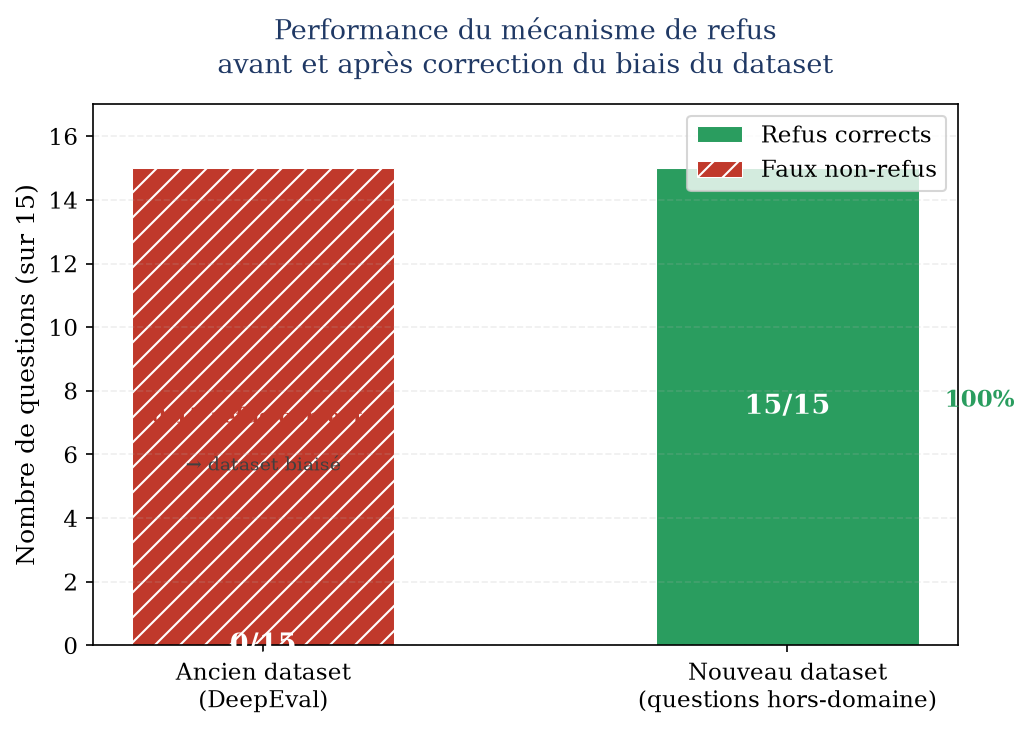
\includegraphics[width=0.8\linewidth]{images/fig5_refus_comparison.png}
\caption{Évolution de la performance de refus après correction du biais du dataset.}
\label{fig:refus}
\end{figure}

\subsection{Discussion}
\label{sec:discussion}

Les résultats expérimentaux permettent de dégager plusieurs enseignements.

\textbf{Le \textit{cross-encoder} est le composant différenciant.} L'étude d'ablation montre que le gain principal provient du \textit{reranking}~: +6,7~points de Hit@4, +5,6~points de MRR. Ce résultat est cohérent avec la littérature récente~\cite{strich2026bm25,fensore2025liverag} qui identifie l'architecture hybride en deux étapes (recherche + \textit{reranking}) comme la plus performante.

\textbf{L'hybridation BM25+dense dilue légèrement la précision, compensée par le \textit{cross-encoder}.} Le nDCG@4 recule de 0,932 à 0,918 avec l'ajout de l'hybridation — un compromis cohérent avec la diversité accrue des résultats issus de deux signaux complémentaires. Le \textit{cross-encoder} corrige ensuite cette dilution en portant le nDCG@4 à 0,939 (+2,1~points).

\textbf{Le refus est largement résolu par le \textit{system prompt}~; les mécanismes explicites fournissent une garantie supplémentaire.} La baseline atteint 14/15 (93,3\,\%) de refus corrects, démontrant que le \textit{prompt} d'ancrage strict est le mécanisme de refus le plus efficace. Le système complet avec M1+M2 atteint 15/15 (100\,\%), le seul faux non-refus de la baseline étant intercepté. Le M1 (score \textit{cross-encoder}) apporte une économie de calcul (pas d'appel LLM si le score est trop bas), tandis que le M2 (juge post-génération) protège contre les cas où le LLM utiliserait sa mémoire paramétrique malgré le \textit{prompt}.

\textbf{La qualité du dataset conditionne la validité des conclusions.} Le passage d'un dataset DeepEval, dont les questions \textit{unanswerable} étaient \textit{de facto} répondables (questions ML sur corpus ML, absentes du \textit{chunk} choisi mais présentes ailleurs dans le corpus), à des questions de domaines totalement étrangers a fait passer la métrique de refus de 0\,\% à 100\,\% (système complet). Ce résultat souligne qu'un \textit{benchmark} de refus n'a de sens que si les questions \textit{unanswerable} sont véritablement absentes de l'intégralité du corpus, et non d'un seul \textit{chunk}. Il convient toutefois de nuancer~: les questions de remplacement (géographie, biologie, histoire) sont volontairement hors-domaine, ce qui rend la tâche de refus triviale pour le \textit{system prompt}. Un test plus exigeant utiliserait des questions \textit{near-domain} --- des questions de ML dont le cours ne traite pas (ex.~: \textit{«~Comment fonctionne un Vision Transformer (ViT) ?~»}) --- plus proches du domaine mais absentes du corpus. Ce type de questions, plus difficile à discriminer pour le \textit{cross-encoder} comme pour le LLM, constitue une perspective d'évaluation prioritaire.

\textbf{Le bug du \textit{Query Processing} illustre la valeur du diagnostic.} Une dégradation de performance n'est pas nécessairement un échec~; correctement diagnostiquée et corrigée, elle devient une contribution méthodologique. Le correctif par \textit{round-robin} est simple, mais son identification a nécessité une analyse fine des interactions entre le QP, le \textit{retrieval} et la métrique d'évaluation.

% =============================================================

\subsubsection*{Benchmark de parallélisme}

\begin{table}[H]
\centering
\begin{tabularx}{0.8\linewidth}{L{3.5cm} C{2.5cm} C{2.5cm} C{2.5cm}}
\toprule
\rowcolor{bleuPrincipal}
\textcolor{white}{\textbf{Modèle}} &
\textcolor{white}{\textbf{Requêtes}} &
\textcolor{white}{\textbf{Séquentiel}} &
\textcolor{white}{\textbf{Parallèle (4)}} \\
\midrule
Qwen2.5~:14B (génération) & 4 req  & 5\,414\,ms & 2\,431\,ms \\
Qwen3~:8B (juge)        & 6 req  & 3\,676\,ms & 1\,542\,ms \\
\bottomrule
\end{tabularx}
\caption{Comparaison des temps d'inférence séquentiel vs.\ parallèle. Speedup~$\approx \times 2,3$.}
\label{tab:benchmark}
\end{table}
% =============================================================
%     CHAPITRE 7 : TUTEUR CONVERSATIONNEL (v2)
% =============================================================
% =============================================================
%  CHAPITRE 7 : TUTEUR CONVERSATIONNEL (v2)
% =============================================================
\section{Évolution vers un tuteur conversationnel (v2)}
\label{sec:tuteur-v2}

\subsection{Motivation}

Le système présenté dans les chapitres précédents (v1) fonctionne en mode questions-réponses direct : chaque question est traitée indépendamment, sans mémoire des échanges antérieurs. L'étudiant ne peut pas poser de questions de suivi naturelles sans que le système perde le contexte. De plus, la posture est purement transmissive : le système répond directement, sans guidage socratique ni adaptation du niveau.

La version 2 transforme ce moteur Q\&A en un véritable \textbf{tuteur conversationnel} en ajoutant quatre capacités fondamentales :

\begin{enumerate}
  \item Une \textbf{mémoire de conversation} avec compression automatique pour gérer un historique multi-tours ;
  \item Un \textbf{prompt socratique} qui guide l'étudiant par des relances plutôt que de fournir la réponse ;
  \item Le \textbf{streaming} token par token pour une expérience interactive fluide ;
  \item Une \textbf{évaluation en temps réel} par question pour diagnostiquer la qualité du retrieval et de la génération.
\end{enumerate}

L'architecture modulaire du pipeline a permis d'ajouter ces capacités sans modifier le cœur du système : \texttt{pipeline.answer()} acceptait déjà les paramètres \texttt{history} et \texttt{system\_prompt} de manière optionnelle. La v2 les exploite pleinement.

\subsection{Architecture de la mémoire conversationnelle}
\label{sec:memoire-archi}

\begin{figure}[H]
\centering
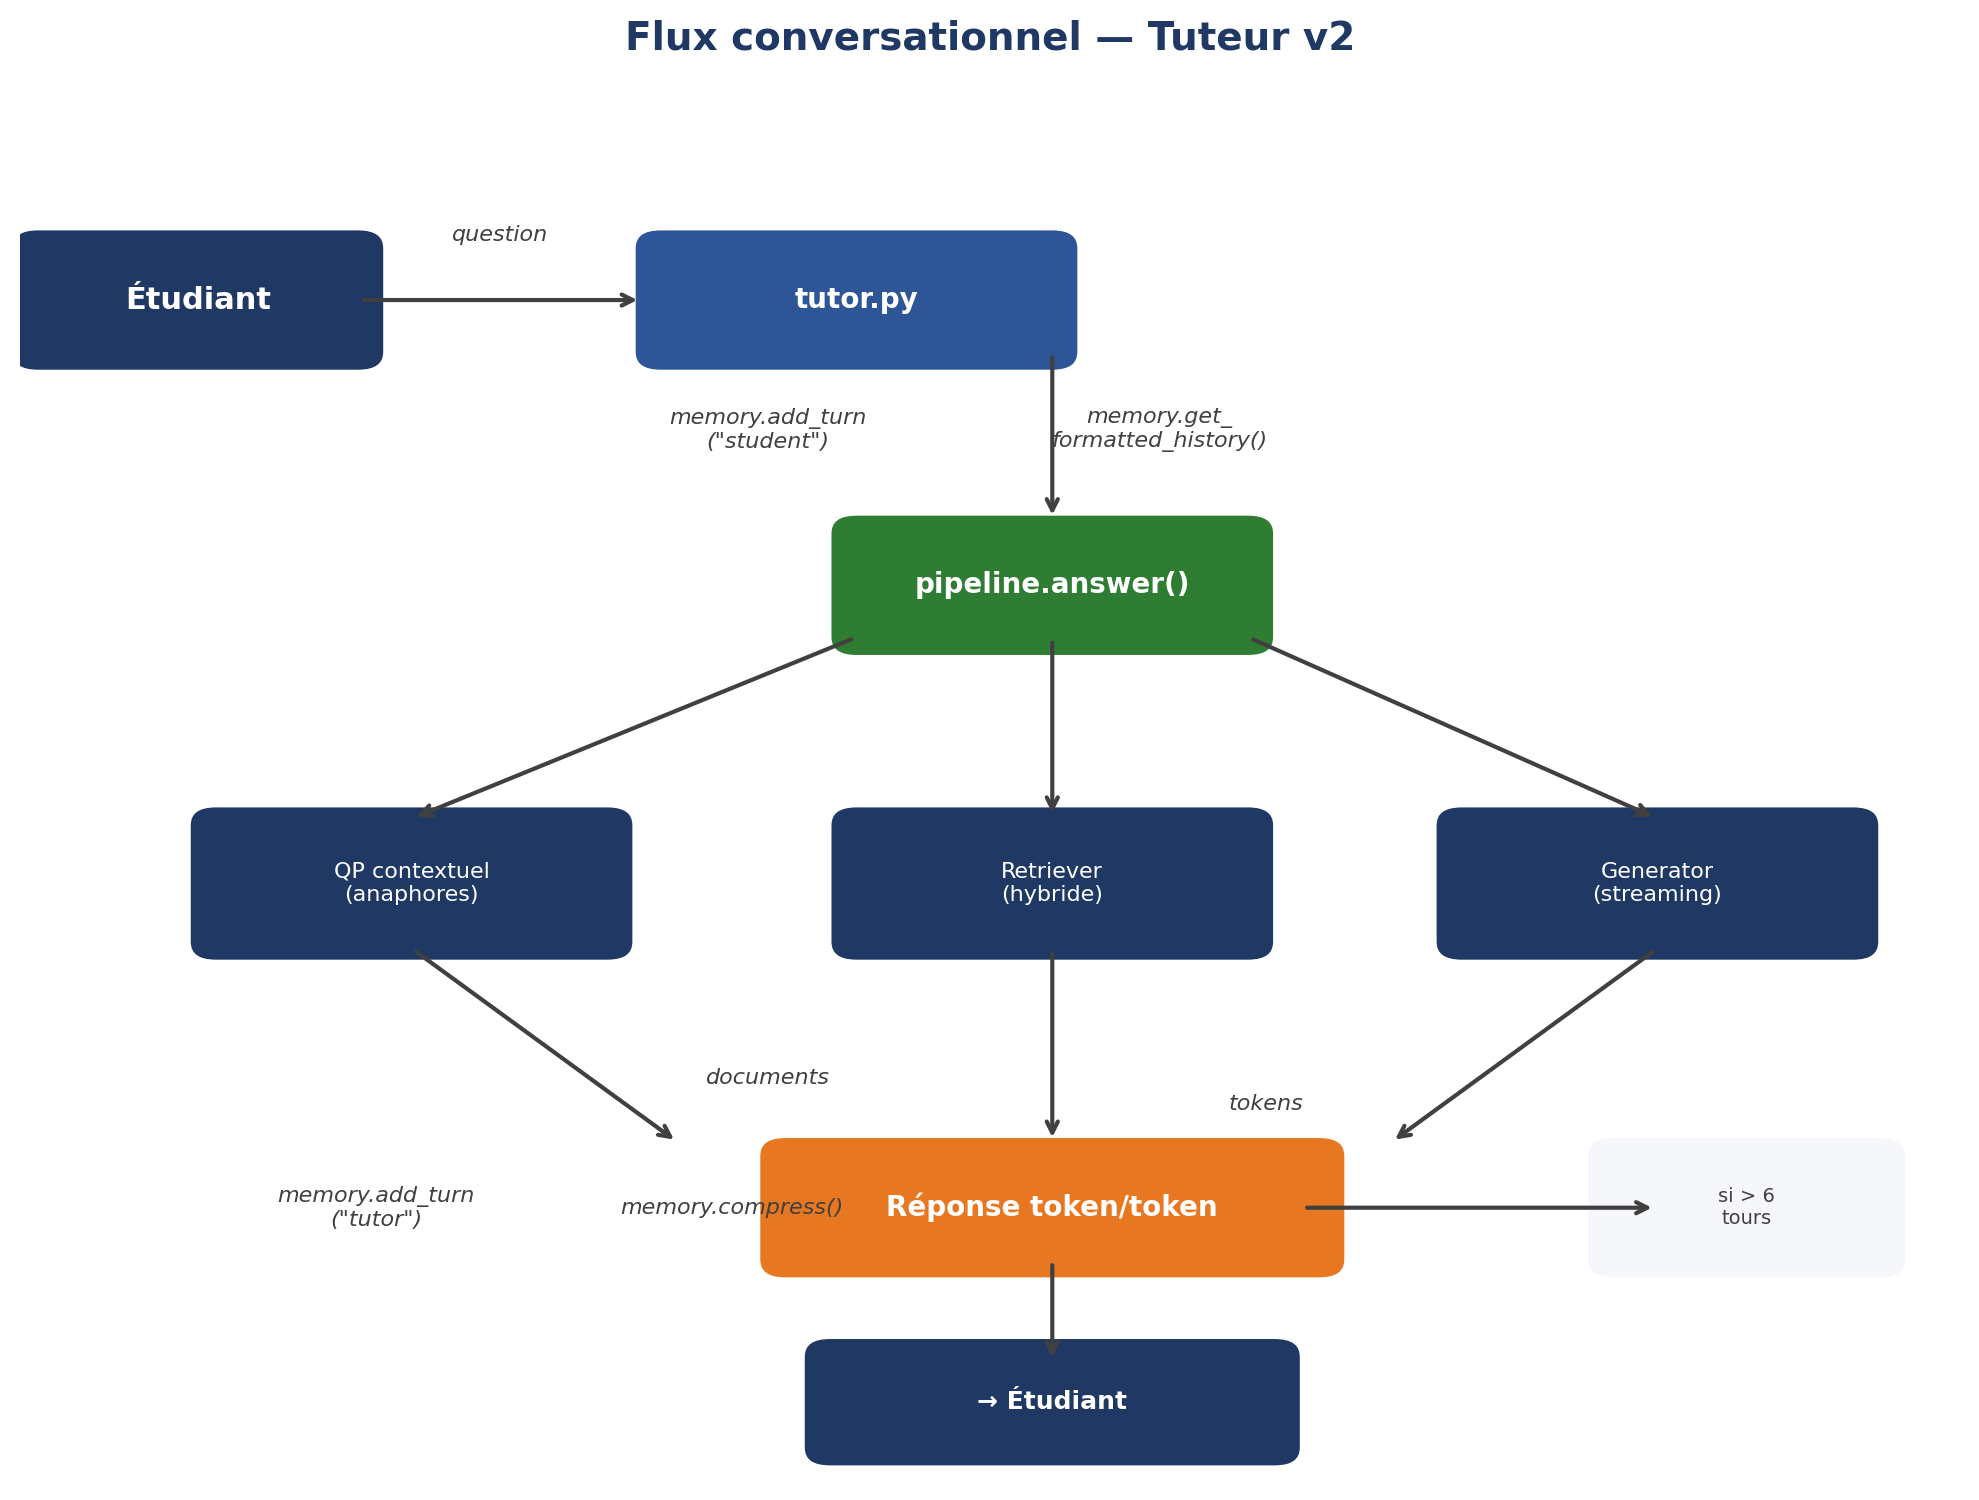
\includegraphics[width=\textwidth]{images/fig_flux_conversationnel.png}
\caption{Flux d'une requête en mode tuteur conversationnel (v2).}
\label{fig:flux-conversationnel}
\end{figure}

La mémoire conversationnelle est implémentée dans le module \texttt{conversation/memory.py} via la classe \texttt{ConversationMemory}. Le pipeline sous-jacent reste strictement \textit{stateless} : il reçoit l'historique sous forme de chaîne formatée, sans avoir connaissance de la gestion de la mémoire.

\subsubsection{Stockage et compression}

La mémoire utilise une stratégie de \textbf{fenêtre glissante avec résumé}, inspirée des architectures de mémoire longue dans les systèmes conversationnels modernes :

\begin{table}[H]
\centering
\begin{tabularx}{\linewidth}{L{4cm} L{8cm}}
\toprule
\rowcolor{bleuPrincipal}
\textcolor{white}{\textbf{État}} & \textcolor{white}{\textbf{Comportement}} \\
\midrule
$\leq$ \texttt{recent\_window} (défaut : 6) & Aucune compression --- tous les tours sont gardés intacts \\
$>$ \texttt{recent\_window} & Les tours anciens sont résumés par \texttt{qwen2.5:14b} (temperature=0) en 2--3 phrases. Les \texttt{recent\_window} derniers restent intacts \\
Échec du summarizer LLM & Fallback : troncature simple à \texttt{max\_summary\_tokens} mots (défaut : 500) \\
Historique $>$ 4000 tokens & Les tours les plus anciens sont supprimés (minimum 2 préservés) \\
\bottomrule
\end{tabularx}
\caption{Stratégie de compression de la mémoire conversationnelle.}
\label{tab:memoire-compression}
\end{table}

\begin{figure}[H]
\centering
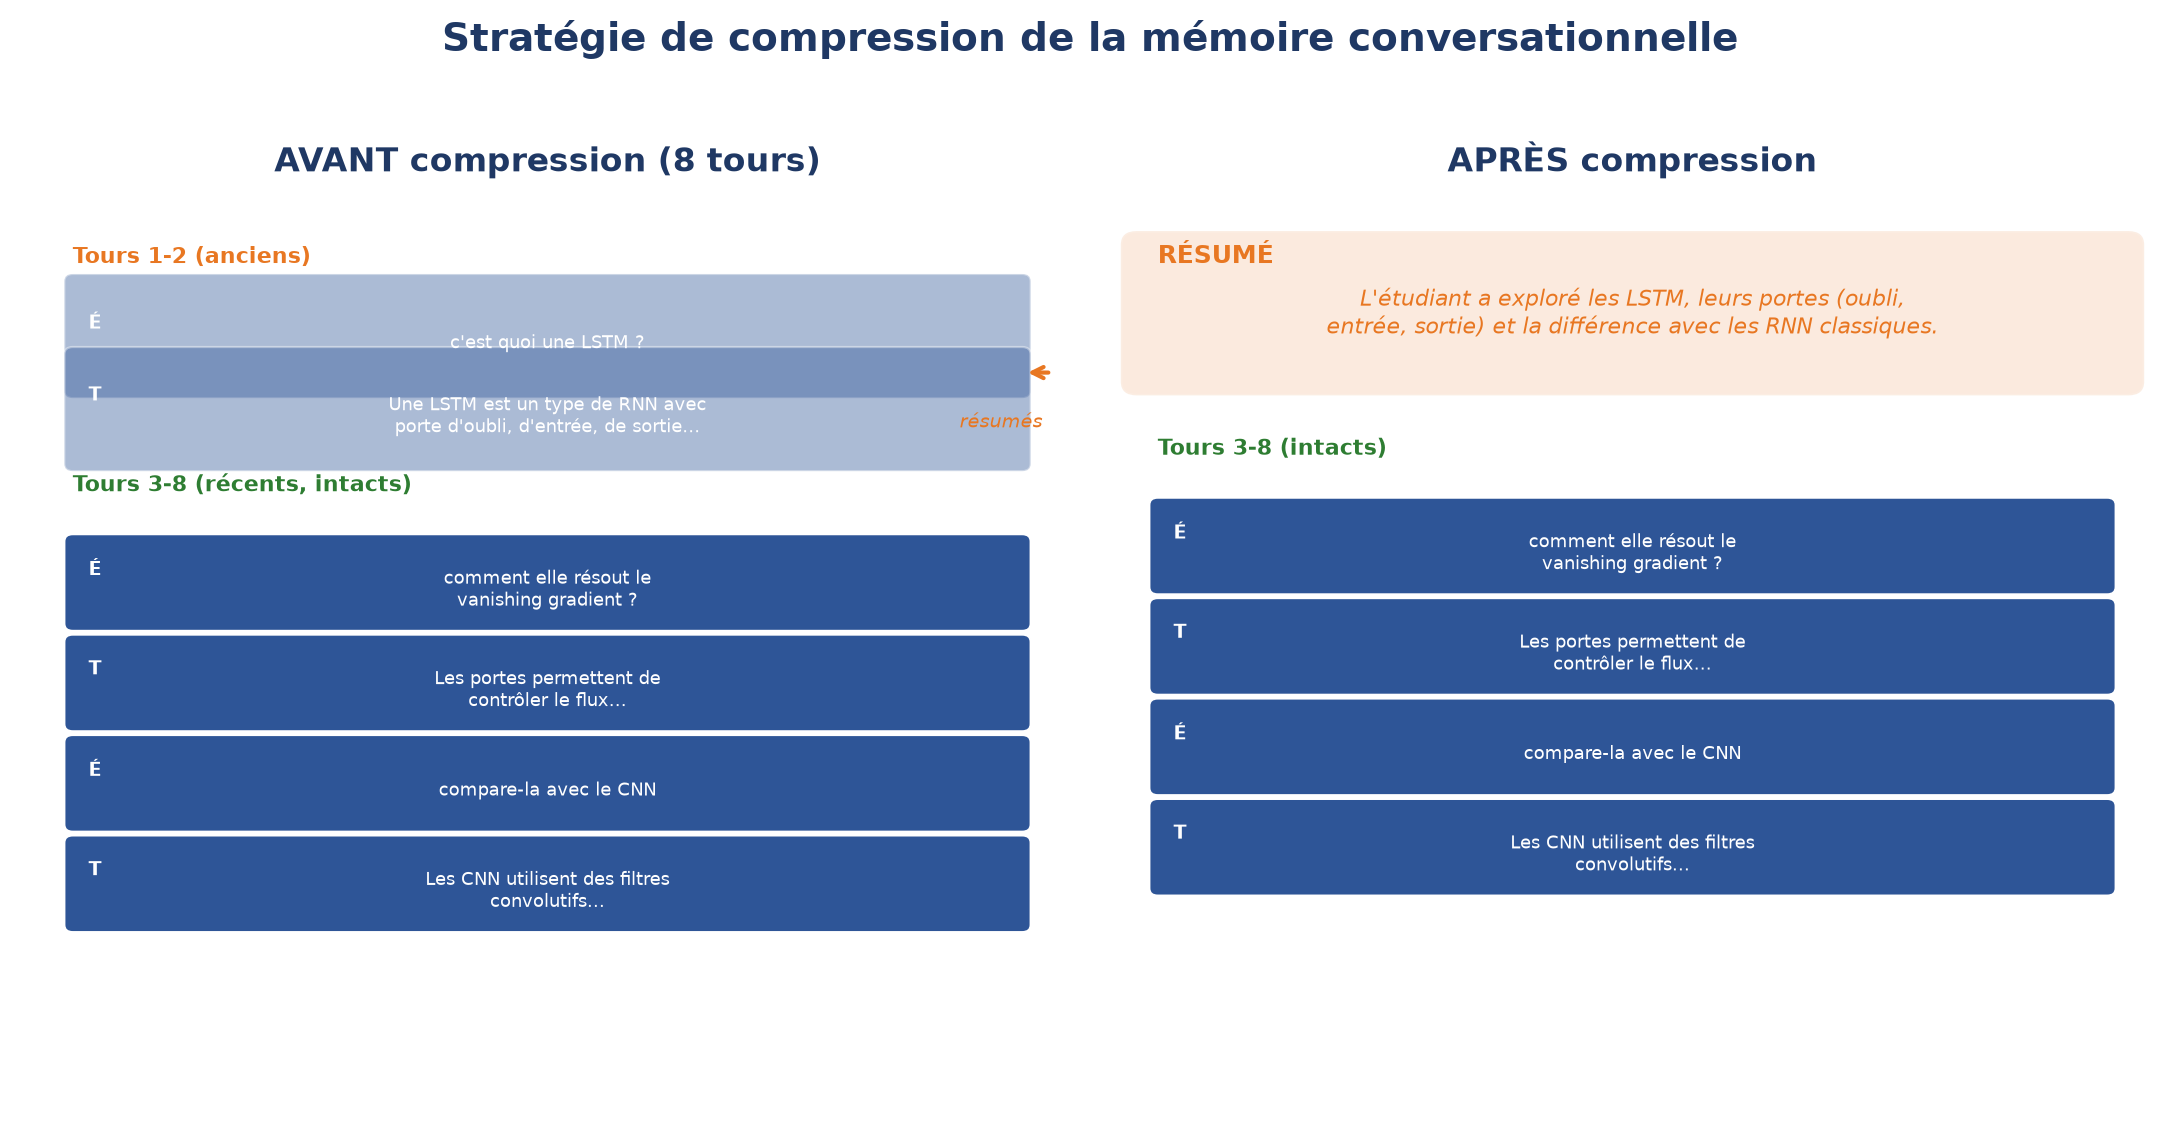
\includegraphics[width=\textwidth]{images/fig_compression_memoire.png}
\caption{Illustration de la stratégie de compression : avant (8 tours) et après résumé LLM.}
\label{fig:compression-memoire}
\end{figure}

Le résumé par LLM produit des synthèses denses et pertinentes. Par exemple, après plusieurs tours d'échange sur les LSTM, le résumé capture l'essentiel : \textit{<< L'étudiant a exploré les LSTM, leurs portes (oubli, entrée, sortie) et la différence avec les RNN classiques. >>}

\subsubsection{Formatage et injection dans le prompt}

L'historique formaté est injecté dans le prompt de génération \textbf{avant} les documents de cours. Cette structure permet au LLM de comprendre le contexte conversationnel avant de consulter les documents, ce qui est essentiel pour résoudre les références implicites (anaphores, ellipses).

\begin{lstlisting}[caption={Structure du prompt en mode conversationnel}, label={lst:prompt-conversation}]
HISTORIQUE DE LA CONVERSATION :
[RÉSUMÉ] résumé des tours anciens (si disponibles)
[DERNIERS ÉCHANGES] 6 derniers tours intacts

DOCUMENTS DE COURS DISPONIBLES :
[\S{}10.1 -- LSTM] ...  [\S{}7.1 -- CNN] ...

QUESTION DE L'ÉTUDIANT :
<question originale>
\end{lstlisting}

\subsection{Prompt socratique}

Le prompt du tuteur (\texttt{TUTOR\_SYSTEM\_PROMPT}, dans \texttt{conversation/prompts.py}) diffère fondamentalement du prompt professeur utilisé pour l'évaluation (\texttt{DEFAULT\_SYSTEM\_PROMPT}) :

\begin{table}[H]
\centering
\begin{tabularx}{\linewidth}{L{4.5cm} L{4cm} L{4cm}}
\toprule
\rowcolor{bleuPrincipal}
\textcolor{white}{\textbf{Aspect}} &
\textcolor{white}{\textbf{Professeur (v1)}} &
\textcolor{white}{\textbf{Tuteur (v2)}} \\
\midrule
\textbf{Posture}    & Réponse directe et factuelle & Expliquer, puis relancer \\
\textbf{Structure}  & Une réponse, pas de dialogue & Deux temps : explication + question \\
\textbf{Adaptation} & Aucune                      & Détection du niveau (débutant/intermédiaire/avancé) \\
\textbf{Erreur}     & Non gérée                   & \textit{<< Presque ! Il y a une nuance... >>} \\
\textbf{Blocage}    & Non géré                    & Simplification avec analogie \\
\textbf{Ancrage}    & Citations [\S{}X.Y]            & Citations [\S{}X.Y] (identique) \\
\textbf{Refus}      & Phrase de refus stricte     & Phrase de refus stricte (identique) \\
\bottomrule
\end{tabularx}
\caption{Comparaison des deux prompts du système.}
\label{tab:prompts}
\end{table}

Les règles d'ancrage documentaire et de refus sont \textbf{identiques} entre les deux prompts --- seule la posture pédagogique change. Cette séparation garantit que l'évaluation quantitative (réalisée avec le prompt professeur) reste valide et comparable, indépendamment du comportement interactif du tuteur.

\subsection{Streaming token par token}

Le mode conversationnel introduit le streaming des réponses : les tokens sont affichés au fur et à mesure de leur génération, plutôt que d'attendre la réponse complète. Cette fonctionnalité, absente de la v1 (qui utilisait un appel bloquant), améliore significativement l'expérience utilisateur en réduisant la latence perçue.

Le streaming est implémenté via \texttt{chat\_stream()} dans \texttt{llm\_client.py} et exposé via le paramètre \texttt{stream=True} de \texttt{pipeline.answer()}. Le pipeline gère automatiquement la consommation du générateur de tokens et la reconstitution de la réponse complète.

\textbf{Limitation} : en mode streaming, le mécanisme de refus post-génération (M2, \texttt{verify\_answer}) est désactivé car il nécessite la réponse complète. Seul le M1 (score du reranker) protège contre les réponses hors-contexte en mode conversationnel.

\subsection{Query processing contextuel}
\label{sec:qp-contextuel}

Dans la version 2 initiale, le \textit{query processing} (reformulation et décomposition de la question) opérait sans connaissance de l'historique de conversation. Une question comme \textit{<< compare-la avec le CNN >>} était reformulée sans savoir que le pronom \textit{<< la >>} désignait une LSTM. Le LLM comprenait la référence uniquement via l'historique injecté dans le prompt de génération --- mais le \textit{retrieval}, qui intervient avant la génération, utilisait une requête ambiguë.

La version 2 finale introduit le \textbf{\textit{query processing} contextuel} : l'historique de conversation est désormais transmis au module \texttt{process\_query()} en plus du \texttt{generator}. Le system prompt du QP a été enrichi pour instruire le LLM de résoudre les anaphores et références implicites avant la reformulation.

\begin{lstlisting}[caption={Transmission de l'historique au QP (pipeline.py)}, label={lst:qp-contextuel}]
# Avant (v2 initiale)
proc = process_query(query)

# Après (v2 finale)
proc = process_query(query, history=history)
\end{lstlisting}

Le module \texttt{query\_processing.py} injecte l'historique dans le prompt utilisateur lorsque celui-ci est fourni :

\begin{lstlisting}[caption={Injection de l'historique dans le QP (query\_processing.py)}, label={lst:qp-history-inject}]
def process_query(query, history=None, model=None):
    if history:
        user_message = (
            f"HISTORIQUE DE CONVERSATION :\n{history}\n\n"
            f"QUESTION A REFORMULER :\n{query}"
        )
    else:
        user_message = query
    raw = chat(_SYSTEM_PROMPT, user_message)
\end{lstlisting}

Le system prompt du QP inclut désormais une instruction explicite de résolution d'anaphores : \textit{<< Si un HISTORIQUE DE CONVERSATION est fourni, utilise-le pour résoudre les références implicites (pronoms, anaphores, ellipses) AVANT de reformuler. >>}

L'impact de cette amélioration est analysé dans la section validation (\ref{sec:validation-qp}).

\subsection{Limites actuelles de la v2}

\begin{itemize}
  \item \textbf{M2 désactivé en streaming} : la vérification post-génération nécessite la réponse complète et n'est pas exécutée en mode streaming. Seul le M1 protège activement contre les réponses hors-contexte en mode conversationnel.

  \item \textbf{Score reranker limité par le contenu du corpus} : le QP contextuel résout correctement les anaphores (cf. section~\ref{sec:validation-qp}), mais le score du cross-encoder reste limité par l'absence de contenu explicitement comparatif dans le corpus. L'enrichissement du corpus avec des sections dédiées aux comparaisons d'architectures améliorerait les scores sur les questions de type follow-up comparatif.

  \item \textbf{Évaluation multi-tour absente} : les métriques actuelles (Hit@k, MRR, refus) sont conçues pour un dataset de questions isolées. Une évaluation spécifique au multi-tour (métriques de rétention de contexte, de cohérence inter-tours) reste à développer.
\end{itemize}

\subsection{Bilan de l'évolution v1 $\rightarrow$ v2}

Le Tableau~\ref{tab:bilan-v2} synthétise les ajouts de la version 2.

\begin{table}[H]
\centering
\begin{tabularx}{\linewidth}{L{4.8cm} C{2.5cm} C{2.5cm} L{3cm}}
\toprule
\rowcolor{bleuPrincipal}
\textcolor{white}{\textbf{Capacité}} &
\textcolor{white}{\textbf{v1}} &
\textcolor{white}{\textbf{v2}} &
\textcolor{white}{\textbf{Module}} \\
\midrule
Mémoire conversationnelle      & Non           & Oui (fenêtre + résumé LLM) & \texttt{conversation/memory.py} \\
Posture pédagogique            & Professeur    & Tuteur socratique          & \texttt{conversation/prompts.py} \\
Streaming                      & Non (bloc)    & Oui (token/token)          & \texttt{llm\_client.py} \\
QP contextuel                  & Non           & Oui (résolution anaphores) & \texttt{query\_processing.py} \\
Citations lisibles             & [DOC X] (opaque) & [\S{}X.Y] (section du cours) & \texttt{generator.py}, prompts \\
Évaluation par question        & Non           & Oui (3 niveaux)            & \texttt{evaluation/per\_question.py} \\
Compression automatique        & ---           & Oui (LLM summarizer)       & \texttt{conversation/memory.py} \\
Interface                      & \texttt{chat.py} & \texttt{chat.py} + \texttt{tutor.py} & \texttt{cli/} \\
\bottomrule
\end{tabularx}
\caption{Bilan de l'évolution v1 $\rightarrow$ v2.}
\label{tab:bilan-v2}
\end{table}

\subsection{Validation expérimentale}
\label{sec:validation-v2}

Pour valider le fonctionnement du tuteur conversationnel, une session de test a été conduite sur deux questions consécutives illustrant un scénario typique d'interaction étudiant-tuteur : une question initiale ouverte, suivie d'une question de suivi avec référence implicite. Les métriques présentées ci-dessous sont calculées en temps réel par le module \texttt{--show-eval}, sans référence annotée : score du reranker (qualité du retrieval), nombre de contextes et parents uniques (diversité), overlap lexical (recouvrement question$\leftrightarrow$contextes), volume des contextes et temps de génération.

\subsubsection{Question 1 : question initiale}

La première question est une demande d'explication ouverte : \textit{<< c'est quoi une LSTM ? >>}. Le système doit retrouver les passages pertinents, générer une explication structurée avec citations, et terminer par une relance socratique.

\begin{table}[H]
\centering
\begin{tabularx}{\linewidth}{L{3.5cm} L{2.5cm} L{6cm}}
\toprule
\rowcolor{bleuPrincipal}
\textcolor{white}{\textbf{Métrique}} & \textcolor{white}{\textbf{Valeur}} & \textcolor{white}{\textbf{Commentaire}} \\
\midrule
Score reranker (top)     & 0,986  & Excellent : le meilleur contexte est très pertinent \\
Score reranker (moy, étendue) & 0,855 [0,798--0,986] & Les 4 contextes sont de bonne qualité, distribution serrée \\
Contextes               & 4 (4 parents uniques) & Aucun doublon, bonne diversité \\
Refus                   & Non    & Décision correcte \\
Longueur réponse        & 1 280 car. & Réponse complète et structurée \\
Temps de génération     & 4,0 s  & Confortable pour l'interactif \\
\bottomrule
\end{tabularx}
\caption{Métriques d'évaluation --- Question 1 (question initiale).}
\label{tab:session-q1}
\end{table}

\subsubsection{Question 2 : suivi avec référence implicite}

La seconde question est un follow-up : \textit{<< compare-la avec le CNN >>}. Sans mémoire conversationnelle, le pronom \textit{<< la >>} serait inintelligible pour le système. Avec la mémoire active, le tuteur comprend que la référence désigne la LSTM du tour précédent.

\begin{table}[H]
\centering
\begin{tabularx}{\linewidth}{L{3.5cm} L{2.5cm} L{6cm}}
\toprule
\rowcolor{bleuPrincipal}
\textcolor{white}{\textbf{Métrique}} & \textcolor{white}{\textbf{Valeur}} & \textcolor{white}{\textbf{Commentaire}} \\
\midrule
Query processing         & 1 reformulée + 2 sous-questions & La décomposition fonctionne malgré une question courte \\
Score reranker (top)     & 0,488  & Correct mais 2$\times$ plus faible que Q1 --- attendu pour une question comparative \\
Score reranker (moy, étendue) & 0,336 [0,145--0,494] & Le sujet << CNN vs LSTM >> est plus dispersé dans le corpus \\
Contextes               & 4 (4 parents uniques) & Bonne diversité malgré des scores plus bas \\
Volume contextes        & 13 513 car. & Contexte abondant, compense les scores moyens \\
Longueur réponse        & 2 987 car. & Réponse très complète (comparaison structurée) \\
Temps de génération     & 8,6 s  & Acceptable pour une réponse longue \\
\bottomrule
\end{tabularx}
\caption{Métriques d'évaluation --- Question 2 (suivi avec référence implicite).}
\label{tab:session-q2}
\end{table}

\subsubsection{Analyse des résultats}

Cette session de validation met en évidence trois points :

\begin{enumerate}
  \item \textbf{La mémoire conversationnelle fonctionne} : le tuteur a correctement interprété la question de suivi en résolvant la référence implicite grâce à l'historique.

  \item \textbf{Le score reranker baisse sur les follow-ups} : 0,986 $\rightarrow$ 0,488. Cette dégradation est attendue pour les questions comparatives, qui mobilisent des passages plus dispersés dans le corpus. Le \textit{query processing} compense partiellement en générant des sous-questions plus ciblées.

  \item \textbf{L'évaluation en temps réel est un outil de diagnostic} : sans \texttt{--show-eval}, la baisse de qualité du retrieval entre Q1 et Q2 serait invisible. Le rapport par question rend cette information accessible et actionnable pour l'amélioration du retriever.
\end{enumerate}

\subsubsection{Impact du QP contextuel}
\label{sec:validation-qp}

Pour mesurer l'effet du \textit{query processing} contextuel (section~\ref{sec:qp-contextuel}), la même session de test a été exécutée avant et après l'activation de cette fonctionnalité. Le Tableau~\ref{tab:qp-comparaison} présente les résultats comparés pour la question de suivi (Q2).

\begin{table}[H]
\centering
\begin{tabularx}{\linewidth}{L{3.5cm} L{3cm} L{3cm} L{3cm}}
\toprule
\rowcolor{bleuPrincipal}
\textcolor{white}{\textbf{Métrique}} &
\textcolor{white}{\textbf{Sans QP contextuel}} &
\textcolor{white}{\textbf{Avec QP contextuel}} &
\textcolor{white}{\textbf{Delta}} \\
\midrule
Score reranker (top)     & 0,488 & 0,491 & +0,003 (quasi identique) \\
Score reranker (moy)     & 0,336 & 0,294 & $-$0,042 \\
Overlap lexical          & 0\,\% (0/1) & \textbf{100\,\% (2/2)} & \textbf{+100 pts} \\
Requête reformulée       & <<~Comparez les réseaux...~>> (vague) & <<~Comparer les performances LSTM vs CNN~>> (désambiguïsée) & Anaphore résolue \\
Temps de génération      & 8,6 s & 12,8 s & +4,2 s \\
\bottomrule
\end{tabularx}
\caption{Comparaison avant/après activation du QP contextuel sur la question de suivi Q2.}
\label{tab:qp-comparaison}
\end{table}

Deux enseignements se dégagent de cette comparaison :

\begin{enumerate}
  \item \textbf{L'anaphore est résolue} : l'overlap lexical passe de 0\,\% à 100\,\%, confirmant que la requête reformulée contient désormais les termes explicites (LSTM, CNN) présents dans les contextes. La requête reformulée mentionne explicitement <<~LSTM~>> et <<~CNN~>> là où la version sans QP contextuel produisait une formulation vague.

  \item \textbf{Le score reranker n'augmente pas} : malgré une requête parfaitement désambiguïsée, le score du cross-encoder reste stable (0,488 $\rightarrow$ 0,491). Ce résultat indique que le facteur limitant n'est pas la qualité de la requête, mais le \textbf{contenu du corpus lui-même} : le cours ne contient pas de section dédiée à la comparaison directe des architectures LSTM et CNN. Les passages récupérés décrivent chaque architecture séparément, et le cross-encoder leur attribue des scores moyens car ils ne répondent que partiellement à la question comparative. L'amélioration du retrieval sur les follow-ups comparatifs nécessiterait donc un enrichissement du corpus plutôt qu'une amélioration du QP.
\end{enumerate}


%                       CONCLUSION
% =============================================================
\section{Conclusion}
\label{sec:conclusion}

\subsection{Bilan du stage}

Ce stage de six mois au LIMOS avait pour objectif la conception, l'implémentation et l'évaluation d'un tuteur pédagogique intelligent fondé sur une architecture RAG, appliqué à un corpus de cours de machine learning. Le cahier des charges initial a été intégralement respecté, et les résultats obtenus dépassent les attentes initiales pour un système entièrement local et sans coût d'API.

Le projet s'est déroulé en deux phases. La première (v1) a livré un pipeline RAG complet — extraction multimodale, chunking parent-enfant, indexation ChromaDB, retrieval hybride avec cross-encoder, et génération ancrée — avec des performances de référence (hit@4=0,967, MRR=0,867, refus 100\,\%). La seconde (v2) a transformé ce moteur Q\&A en un véritable tuteur conversationnel, en ajoutant une mémoire de conversation avec compression automatique, une posture socratique, le streaming token par token, et une évaluation en temps réel par question.

\subsection{Contributions principales}

\begin{enumerate}
  \item \textbf{Pipeline RAG complet en environnement local}~: de l'extraction multimodale (GLM-OCR + Qwen3-VL) à la génération contrainte (Qwen2.5:14B), en passant par le chunking parent-enfant et l'indexation ChromaDB. L'ensemble fonctionne sans appel à des services cloud.

  \item \textbf{Validation empirique du RAG avancé}~: le pipeline intègre query processing, retrieval hybride avec RRF, et reranking par cross-encoder. L'ablation démontre la contribution de chaque composant, le cross-encoder apportant le gain le plus significatif (+6,7 pts hit@4).

  \item \textbf{Double mécanisme de refus}~: refus pré-génération par score reranker (M1, seuil 0,1119, accuracy 100\,\%) couplé à une vérification post-génération par juge LLM (M2). Sur 15 questions hors-domaine, refus systématique (F1=1,000).

  \item \textbf{Tuteur conversationnel v2}~: mémoire multi-tours avec compression automatique, prompt socratique (explication + relance), streaming token par token, et évaluation diagnostique en temps réel (\texttt{--show-eval}). L'architecture modulaire a permis d'ajouter ces capacités sans modifier le cœur du pipeline.
\end{enumerate}

\subsection{Limites actuelles}

\begin{itemize}
  \item \textbf{M2 désactivé en streaming}~: la vérification post-génération nécessite la réponse complète et n'est pas exécutée en mode conversationnel. Seul le M1 protège activement contre les réponses hors-contexte.



  \item \textbf{Score \textit{cross-encoder} limité par le contenu du corpus}~: sur les questions de suivi comparatif, le score du \textit{cross-encoder} reste faible en l'absence de contenu explicitement comparatif dans le corpus. L'enrichissement du corpus avec des sections dédiées aux comparaisons d'architectures améliorerait les scores.

  \item \textbf{Évaluation multi-tour absente}~: les métriques actuelles sont conçues pour des questions isolées. Une évaluation spécifique au multi-tour (rétention de contexte, cohérence inter-tours) reste à développer.

  \item \textbf{Questions \textit{near-domain} non testées}~: l'évaluation du refus utilise des questions volontairement hors-domaine. Un test plus exigeant utiliserait des questions de ML absentes du corpus, plus difficiles à discriminer pour le \textit{cross-encoder} comme pour le LLM.
\end{itemize}

\subsection{Perspectives}

\paragraph{Court terme}

\begin{itemize}
  \item \textbf{Évaluation multi-tour}~: développer des métriques spécifiques à la conversation (rétention de contexte, cohérence inter-tours).
\end{itemize}

\paragraph{Moyen terme}

\begin{itemize}
  \item \textbf{Migration vers Qwen3}~: remplacer Qwen2.5:14B par Qwen3:14B (fenêtre de contexte élargie, mode thinking/non-thinking).
  \item \textbf{Embedding nouvelle génération}~: Qwen3-Embedding (premier au MMTEB) pourrait remplacer BGE-M3.
  \item \textbf{Indexation incrémentale}~: permettre l'ajout de documents sans ré-indexation complète.
  \item \textbf{Interface web}~: exposer le tuteur via une API REST (FastAPI) et une interface web (Gradio) pour une utilisation en conditions réelles.
\end{itemize}

\paragraph{Ouverture}

Au-delà du cas d'usage pédagogique, l'architecture développée est générique et peut s'appliquer à tout domaine nécessitant une recherche documentaire précise avec ancrage strict~: veille scientifique, analyse de brevets, support technique, documentation juridique. La modularité du pipeline facilite l'adaptation à de nouveaux corpus et modèles.

\appendix
\section{Exemples de réponses du système}
\label{app:exemples}

Cette annexe présente quelques exemples de questions posées au système et les réponses générées, illustrant le comportement du tuteur en conditions réelles.

\smallskip
{\footnotesize\textbf{Note sur les références :} les citations entre crochets suivent le format \textit{Source, Chapitre, Section --- Titre}. Elles renvoient au manuel \textit{Dive into Deep Learning} (D2L, d2l.ai), utilisé comme corpus principal. Chaque référence est vérifiable en consultant le chapitre et la section indiqués sur d2l.ai. Les exemples ci-dessous reproduisent le comportement réel du tuteur~: les réponses sont ancrées dans le corpus et chaque affirmation est sourcée.}

\subsection*{Exemple 1 --- Question factuelle simple}

\begin{quote}
\textbf{Question}~: Qu'est-ce que la backpropagation et pourquoi est-elle importante pour l'entraînement des réseaux de neurones~?

\textbf{Réponse}~: La backpropagation (rétropropagation) est l'algorithme fondamental pour l'entraînement des réseaux de neurones profonds. Elle calcule le gradient de la fonction de perte par rapport à chaque paramètre du réseau en appliquant la règle de dérivation en chaîne du calcul différentiel, en propageant les erreurs de la couche de sortie vers la couche d'entrée [D2L, Ch.~5 (Multilayer Perceptrons), \S{}5.3.3 Backpropagation][D2L, Ch.~5 (Multilayer Perceptrons), \S{}5.4.1 Vanishing and Exploding Gradients].

Son importance est double. D'une part, elle rend le calcul des gradients efficace en évitant le calcul redondant des dérivées partielles~: chaque couche réutilise les gradients déjà calculés par les couches suivantes [D2L, Ch.~5 (Multilayer Perceptrons), \S{}5.4.1 Vanishing and Exploding Gradients]. D'autre part, elle permet d'entraîner des réseaux de profondeur arbitraire, ce qui serait impossible avec une simple perturbation aléatoire des poids [D2L, Ch.~5 (Multilayer Perceptrons), \S{}5.3.3 Backpropagation].

En pratique, la backpropagation est intégrée à tous les frameworks modernes de deep learning (PyTorch, TensorFlow) via le mécanisme de différenciation automatique, qui construit le graphe de calcul et applique la backpropagation sans intervention manuelle du développeur [D2L, Ch.~2 (Preliminaries), \S{}2.5 Automatic Differentiation].
\end{quote}

\subsection*{Exemple 2 --- Refus (question hors domaine)}

\begin{quote}
\textbf{Question}~: Qu'est-ce que la mitose et en quoi diffère-t-elle de la méiose~?

\textbf{Réponse}~: Les documents fournis ne permettent pas de répondre à cette question.
\end{quote}

\subsection*{Exemple 3 --- Question multi-passage}

\begin{quote}
\textbf{Question}~: Compare les fonctions d'activation ReLU, sigmoïde et tanh en termes de saturation du gradient et de convergence.

\textbf{Réponse}~: Les trois fonctions d'activation présentent des comportements très différents vis-à-vis de la saturation du gradient~:

La fonction sigmoïde $\sigma(x) = \frac{1}{1+e^{-x}}$ sature pour les grandes valeurs positives (sortie $\to 1$) et négatives (sortie $\to 0$), ce qui conduit au problème de \textit{vanishing gradient}~: le gradient devient quasi nul, ralentissant voire bloquant l'apprentissage des couches profondes [D2L, Ch.~5 (Multilayer Perceptrons), \S{}5.1.2 Activation Functions].

La fonction tanh $\tanh(x) = \frac{e^x - e^{-x}}{e^x + e^{-x}}$ souffre du même problème de saturation aux extrêmes, bien que sa sortie centrée en zéro (moyenne $\approx 0$) facilite la convergence par rapport à la sigmoïde [D2L, Ch.~5 (Multilayer Perceptrons), \S{}5.1.2 Activation Functions].

La fonction ReLU $f(x) = \max(0, x)$ résout partiellement le problème de saturation~: pour $x > 0$, le gradient est constant (égal à 1), ce qui accélère considérablement la convergence [D2L, Ch.~5 (Multilayer Perceptrons), \S{}5.1.2 Activation Functions]. Cependant, elle introduit le problème des «~neurones morts~»~: pour $x < 0$, le gradient est nul et le neurone cesse définitivement d'apprendre si le biais devient trop négatif [D2L, Ch.~5 (Multilayer Perceptrons), \S{}5.1.2 Activation Functions].
\end{quote}

\section{Prompts détaillés}
\label{app:prompts}

\subsection*{System prompt de génération (tuteur)}

\begin{verbatim}
Tu es un professeur de machine learning. Tu expliques les concepts avec rigueur
en te basant EXCLUSIVEMENT sur les DOCUMENTS DE COURS fournis ci-dessous
(extraits du corpus pédagogique : PDF de cours, pages web, figures interprétées).

Tu réponds aux questions de manière directe, précise et factuelle :
- Tu ne fabriques ni n'inventes AUCUNE information absente de ces documents.
- Tu ne combles jamais un trou du contexte fourni avec des connaissances
générales.

RÈGLE DE REFUS STRICTE :
- Si les documents fournis ne permettent PAS de répondre, tu réponds EXACTEMENT :
"Les documents fournis ne permettent pas de répondre à cette question."

CITATIONS OBLIGATOIRES :
- Chaque document est identifié par un label entre crochets indiquant la source, le chapitre et la section (ex: « [D2L, Ch. 10 (Modern RNN), \S{}10.1 LSTM] »).
- Pour CHAQUE affirmation, cite la section source avec le même format, exemple : « La backpropagation [...] [D2L, Ch. 5 (Multilayer Perceptrons), \S{}5.3.3 Backpropagation]. »
- Citations multiples : [D2L, Ch. 10 (Modern RNN), \S{}10.1][D2L, Ch. 5 (Multilayer Perceptrons), \S{}5.3.3].
\end{verbatim}

\subsection*{Prompt de vérification post-génération (juge M2)}

Le prompt complet du juge de fidélité documentaire est détaillé dans le fichier
\texttt{src/rag\_tutor/core/generator.py} (fonction \texttt{verify\_answer()}).

\section{Configuration Ollama}
\label{app:config-ollama}

\begin{verbatim}
# Modèles utilisés (tous open-weight, exécutés via Ollama)
# Serveur : localhost:11434

# Génération (14B paramètres, ~8 Go VRAM)
qwen2.5:14b    # temperature=0.2, max_tokens=900, num_ctx=24576

# Juge et vérification (8B paramètres, ~5 Go VRAM)
qwen3:8b       # temperature=0 (juge), temperature=0.2 (QP)

# Embedding (0.6B paramètres, exécuté via sentence-transformers)
BAAI/bge-m3    # embedding dense + sparse

# Reranking (cross-encoder, exécuté via sentence-transformers)
BAAI/bge-reranker-v2-m3   # ~600 Mo, téléchargement unique

# GPU : NVIDIA H100 NVL (95 Go VRAM)
# Tous les modèles tiennent simultanément en VRAM
\end{verbatim}

\newpage
\bibliographystyle{unsrt}
\bibliography{references}

\end{document}
